\documentclass[]{book}
\usepackage{lmodern}
\usepackage{amssymb,amsmath}
\usepackage{ifxetex,ifluatex}
\usepackage{fixltx2e} % provides \textsubscript
\ifnum 0\ifxetex 1\fi\ifluatex 1\fi=0 % if pdftex
  \usepackage[T1]{fontenc}
  \usepackage[utf8]{inputenc}
\else % if luatex or xelatex
  \ifxetex
    \usepackage{mathspec}
  \else
    \usepackage{fontspec}
  \fi
  \defaultfontfeatures{Ligatures=TeX,Scale=MatchLowercase}
\fi
% use upquote if available, for straight quotes in verbatim environments
\IfFileExists{upquote.sty}{\usepackage{upquote}}{}
% use microtype if available
\IfFileExists{microtype.sty}{%
\usepackage{microtype}
\UseMicrotypeSet[protrusion]{basicmath} % disable protrusion for tt fonts
}{}
\usepackage[margin=1in]{geometry}
\usepackage{hyperref}
\hypersetup{unicode=true,
            pdftitle={An Example Predictive Modeling Workflow Using The Zillow Prize Dataset},
            pdfauthor={Jesse Piburn},
            pdfborder={0 0 0},
            breaklinks=true}
\urlstyle{same}  % don't use monospace font for urls
\usepackage{natbib}
\bibliographystyle{apalike}
\usepackage{color}
\usepackage{fancyvrb}
\newcommand{\VerbBar}{|}
\newcommand{\VERB}{\Verb[commandchars=\\\{\}]}
\DefineVerbatimEnvironment{Highlighting}{Verbatim}{commandchars=\\\{\}}
% Add ',fontsize=\small' for more characters per line
\usepackage{framed}
\definecolor{shadecolor}{RGB}{248,248,248}
\newenvironment{Shaded}{\begin{snugshade}}{\end{snugshade}}
\newcommand{\KeywordTok}[1]{\textcolor[rgb]{0.13,0.29,0.53}{\textbf{#1}}}
\newcommand{\DataTypeTok}[1]{\textcolor[rgb]{0.13,0.29,0.53}{#1}}
\newcommand{\DecValTok}[1]{\textcolor[rgb]{0.00,0.00,0.81}{#1}}
\newcommand{\BaseNTok}[1]{\textcolor[rgb]{0.00,0.00,0.81}{#1}}
\newcommand{\FloatTok}[1]{\textcolor[rgb]{0.00,0.00,0.81}{#1}}
\newcommand{\ConstantTok}[1]{\textcolor[rgb]{0.00,0.00,0.00}{#1}}
\newcommand{\CharTok}[1]{\textcolor[rgb]{0.31,0.60,0.02}{#1}}
\newcommand{\SpecialCharTok}[1]{\textcolor[rgb]{0.00,0.00,0.00}{#1}}
\newcommand{\StringTok}[1]{\textcolor[rgb]{0.31,0.60,0.02}{#1}}
\newcommand{\VerbatimStringTok}[1]{\textcolor[rgb]{0.31,0.60,0.02}{#1}}
\newcommand{\SpecialStringTok}[1]{\textcolor[rgb]{0.31,0.60,0.02}{#1}}
\newcommand{\ImportTok}[1]{#1}
\newcommand{\CommentTok}[1]{\textcolor[rgb]{0.56,0.35,0.01}{\textit{#1}}}
\newcommand{\DocumentationTok}[1]{\textcolor[rgb]{0.56,0.35,0.01}{\textbf{\textit{#1}}}}
\newcommand{\AnnotationTok}[1]{\textcolor[rgb]{0.56,0.35,0.01}{\textbf{\textit{#1}}}}
\newcommand{\CommentVarTok}[1]{\textcolor[rgb]{0.56,0.35,0.01}{\textbf{\textit{#1}}}}
\newcommand{\OtherTok}[1]{\textcolor[rgb]{0.56,0.35,0.01}{#1}}
\newcommand{\FunctionTok}[1]{\textcolor[rgb]{0.00,0.00,0.00}{#1}}
\newcommand{\VariableTok}[1]{\textcolor[rgb]{0.00,0.00,0.00}{#1}}
\newcommand{\ControlFlowTok}[1]{\textcolor[rgb]{0.13,0.29,0.53}{\textbf{#1}}}
\newcommand{\OperatorTok}[1]{\textcolor[rgb]{0.81,0.36,0.00}{\textbf{#1}}}
\newcommand{\BuiltInTok}[1]{#1}
\newcommand{\ExtensionTok}[1]{#1}
\newcommand{\PreprocessorTok}[1]{\textcolor[rgb]{0.56,0.35,0.01}{\textit{#1}}}
\newcommand{\AttributeTok}[1]{\textcolor[rgb]{0.77,0.63,0.00}{#1}}
\newcommand{\RegionMarkerTok}[1]{#1}
\newcommand{\InformationTok}[1]{\textcolor[rgb]{0.56,0.35,0.01}{\textbf{\textit{#1}}}}
\newcommand{\WarningTok}[1]{\textcolor[rgb]{0.56,0.35,0.01}{\textbf{\textit{#1}}}}
\newcommand{\AlertTok}[1]{\textcolor[rgb]{0.94,0.16,0.16}{#1}}
\newcommand{\ErrorTok}[1]{\textcolor[rgb]{0.64,0.00,0.00}{\textbf{#1}}}
\newcommand{\NormalTok}[1]{#1}
\usepackage{longtable,booktabs}
\usepackage{graphicx,grffile}
\makeatletter
\def\maxwidth{\ifdim\Gin@nat@width>\linewidth\linewidth\else\Gin@nat@width\fi}
\def\maxheight{\ifdim\Gin@nat@height>\textheight\textheight\else\Gin@nat@height\fi}
\makeatother
% Scale images if necessary, so that they will not overflow the page
% margins by default, and it is still possible to overwrite the defaults
% using explicit options in \includegraphics[width, height, ...]{}
\setkeys{Gin}{width=\maxwidth,height=\maxheight,keepaspectratio}
\IfFileExists{parskip.sty}{%
\usepackage{parskip}
}{% else
\setlength{\parindent}{0pt}
\setlength{\parskip}{6pt plus 2pt minus 1pt}
}
\setlength{\emergencystretch}{3em}  % prevent overfull lines
\providecommand{\tightlist}{%
  \setlength{\itemsep}{0pt}\setlength{\parskip}{0pt}}
\setcounter{secnumdepth}{5}
% Redefines (sub)paragraphs to behave more like sections
\ifx\paragraph\undefined\else
\let\oldparagraph\paragraph
\renewcommand{\paragraph}[1]{\oldparagraph{#1}\mbox{}}
\fi
\ifx\subparagraph\undefined\else
\let\oldsubparagraph\subparagraph
\renewcommand{\subparagraph}[1]{\oldsubparagraph{#1}\mbox{}}
\fi

%%% Use protect on footnotes to avoid problems with footnotes in titles
\let\rmarkdownfootnote\footnote%
\def\footnote{\protect\rmarkdownfootnote}

%%% Change title format to be more compact
\usepackage{titling}

% Create subtitle command for use in maketitle
\newcommand{\subtitle}[1]{
  \posttitle{
    \begin{center}\large#1\end{center}
    }
}

\setlength{\droptitle}{-2em}
  \title{An Example Predictive Modeling Workflow Using The Zillow Prize Dataset}
  \pretitle{\vspace{\droptitle}\centering\huge}
  \posttitle{\par}
  \author{Jesse Piburn}
  \preauthor{\centering\large\emph}
  \postauthor{\par}
  \predate{\centering\large\emph}
  \postdate{\par}
  \date{2018-07-21}

\usepackage{booktabs}

\usepackage{amsthm}
\newtheorem{theorem}{Theorem}[chapter]
\newtheorem{lemma}{Lemma}[chapter]
\theoremstyle{definition}
\newtheorem{definition}{Definition}[chapter]
\newtheorem{corollary}{Corollary}[chapter]
\newtheorem{proposition}{Proposition}[chapter]
\theoremstyle{definition}
\newtheorem{example}{Example}[chapter]
\theoremstyle{definition}
\newtheorem{exercise}{Exercise}[chapter]
\theoremstyle{remark}
\newtheorem*{remark}{Remark}
\newtheorem*{solution}{Solution}
\begin{document}
\maketitle

{
\setcounter{tocdepth}{1}
\tableofcontents
}
\chapter*{Welcome}\label{welcome}
\addcontentsline{toc}{chapter}{Welcome}

\begin{figure}
\centering

\includegraphics{zillowprize-png.png}
\caption{Zillow Prize}
\end{figure}

This book is meant to be an illustrative guide for approaching a
predictive modeling task. We'll step through the different parts of the
modeling workflow and work through the Zillow Prize Kaggle Competition
dataset and prediction tasks.

The Github source for this document can be found
\href{https://github.com/jpiburn/zillow-prize}{here}

\chapter{Introduction}\label{intro}

This project is meant to serve as an example workflow for making
predictive models. The sections of the book are roughly broken into the
major steps that are a part of the modeling process.

As with many things in life, their is rarely a one-size-fits-all, always
correct, way of doing something and making a predictive model is no
different. In light of that, I want to stress that the workflow and
methods used in this book are meant to be illustrative not
authoritative.

The only always correct answer in predictive modeling is, ``It
depends.''

\section{Problem}\label{problem}

The problem we will workthrough in this book is the
\href{https://www.kaggle.com/c/zillow-prize-1}{Zillow Prize}
compeitition on that took place on Kaggle. Although it is now closed, it
provides a good problemset for us to work through.

From the site \textgreater{} In this million-dollar competition,
participants will develop an algorithm that makes predictions about the
future sale prices of homes. The contest is structured into two rounds,
the qualifying round which opens May 24, 2017 and the private round for
the 100 top qualifying teams that opens on Feb 1st, 2018. In the
qualifying round, you'll be building a model to improve the Zestimate
residual error. In the final round, you'll build a home valuation
algorithm from the ground up, using external data sources to help
engineer new features that give your model an edge over the competition.

\section{Evaluation}\label{evaluation}

The submission were evaluated based on the Mean Absolute Error between
the predicted \texttt{logerror} and the actual \texttt{logerror}

The \texttt{logerror} is defined as

\begin{equation}
logerror = log(Zestimate) - log(SalePrice)
\label{eq:logerror}
\end{equation}

while Mean Absolute Error is defined as

\begin{equation}
MAE = \frac{{\sum_{i=1}^{n} |y_i - x_i|}}{n} = \frac{{\sum_{i=1}^{n} |e_i|}}{n}
\label{eq:mae}
\end{equation}

\section{Initital Thoughts}\label{initital-thoughts}

\begin{quote}
``Location, Location, Location.''

--- Some Real Estate Guy
\end{quote}

The above quote is of course the number one rule of real estate. Through
out this modeling process, let's try to keep this idea in mind when we
are exploring, creating new features, and modeling the data.

An additional interesting thing about this problem is that it can be
thought about as creating a model to predict where Zillow's model is
bad. We aren't trying to predict home prices, we are predicting where
Zillow had a bad estimate of home prices, so the residuals of their
Zestimate model.Based on this idea, let's create some new features

\section{Note on Using External
Features}\label{note-on-using-external-features}

In the original competition, you were only allowed to use the features
transformations of those included in the data they provided. Since our
goal is to provide an illustrative workflow for making a predictive
model in general and not actually competing in the competition, we are
not going to adhere to that rule and use a few external sources of
information.

\chapter{PreProcessing}\label{preprocessing}

The first step for any data driven project is getting to know the data.
In this section we will look at the raw data that was provided by the
competition and then do a little pre processing that will make the data
easier to work with for the rest of the project

\section{The Raw Data}\label{the-raw-data}

The raw data from zillow contains the following data (desrciptions from
the the data page)

\begin{itemize}
\item
  \textbf{properties\_2016.csv} - all the properties with their home
  features for 2016. Note: Some 2017 new properties don't have any data
  yet except for their parcelid's. Those data points should be populated
  when properties\_2017.csv is available.
\item
  \textbf{properties\_2017.csv} - all the properties with their home
  features for 2017 (released on 10/2/2017)
\item
  \textbf{train\_2016.csv} - the training set with transactions from
  1/1/2016 to 12/31/2016
\item
  \textbf{train\_2017.csv} - the training set with transactions from
  1/1/2017 to 9/15/2017 (released on 10/2/2017)
\item
  \textbf{sample\_submission.csv} - a sample submission file in the
  correct format
\item
  \textbf{zillow\_data\_dictionary.xlsx} - Field Definitions and coded
  value meanings
\end{itemize}

\subsection{\texorpdfstring{Saving Raw Data Using
\texttt{feather}}{Saving Raw Data Using feather}}\label{saving-raw-data-using-feather}

The R binding for the \href{https://github.com/wesm/feather}{feather}
data store provides the ability for very fast read and write of data.
For speed purposes we will save all raw data into a \texttt{.feather}
file format to make all other read faster

\begin{Shaded}
\begin{Highlighting}[]
\KeywordTok{library}\NormalTok{(feather)}
\KeywordTok{library}\NormalTok{(readr)}

\KeywordTok{dir.create}\NormalTok{(}\StringTok{"data-raw/feather"}\NormalTok{)}

\NormalTok{prop_}\DecValTok{16}\NormalTok{ <-}\StringTok{ }\KeywordTok{read_csv}\NormalTok{(}\StringTok{"data-raw/properties_2016.csv"}\NormalTok{)}
\NormalTok{prop_}\DecValTok{17}\NormalTok{ <-}\StringTok{ }\KeywordTok{read_csv}\NormalTok{(}\StringTok{"data-raw/properties_2017.csv"}\NormalTok{)}
\NormalTok{train_}\DecValTok{16}\NormalTok{ <-}\StringTok{ }\KeywordTok{read_csv}\NormalTok{(}\StringTok{"data-raw/train_2016_v2.csv"}\NormalTok{)}
\NormalTok{train_}\DecValTok{17}\NormalTok{ <-}\StringTok{ }\KeywordTok{read_csv}\NormalTok{(}\StringTok{"data-raw/train_2017.csv"}\NormalTok{)}

\KeywordTok{write_feather}\NormalTok{(prop_}\DecValTok{16}\NormalTok{, }\StringTok{"data-raw/feather/properties_2016.feather"}\NormalTok{)}
\KeywordTok{write_feather}\NormalTok{(prop_}\DecValTok{17}\NormalTok{, }\StringTok{"data-raw/feather/properties_2017.feather"}\NormalTok{)}
\KeywordTok{write_feather}\NormalTok{(train_}\DecValTok{16}\NormalTok{, }\StringTok{"data-raw/feather/train_2016_v2.feather"}\NormalTok{)}
\KeywordTok{write_feather}\NormalTok{(train_}\DecValTok{17}\NormalTok{, }\StringTok{"data-raw/feather/train_2017.feather"}\NormalTok{)}
\end{Highlighting}
\end{Shaded}

\section{Renaming Variables}\label{renaming-variables}

Many of the feature names are not very consistant. To take advatange of
helpful functions from the \texttt{tidyverse} set of packages, such as
\texttt{starts\_with()} and \texttt{one\_of()} Let's rename them to
something more consistant and easier to work with.

\subsection{\texorpdfstring{Renaming \texttt{properties}
Features}{Renaming properties Features}}\label{renaming-properties-features}

\begin{Shaded}
\begin{Highlighting}[]
\KeywordTok{library}\NormalTok{(tidyverse)}

\NormalTok{prop_}\DecValTok{16}\NormalTok{ <-}\StringTok{ }\KeywordTok{read_feather}\NormalTok{(}\StringTok{"data-raw/feather/properties_2016.feather"}\NormalTok{)}
\NormalTok{prop_}\DecValTok{17}\NormalTok{ <-}\StringTok{ }\KeywordTok{read_feather}\NormalTok{(}\StringTok{"data-raw/feather/properties_2017.feather"}\NormalTok{)}

\NormalTok{prop_}\DecValTok{16}\NormalTok{ <-}\StringTok{ }\NormalTok{prop_}\DecValTok{16} \OperatorTok\StringTok{ }
\StringTok{  }\KeywordTok{rename}\NormalTok{(}
    \DataTypeTok{id_parcel =}\NormalTok{ parcelid,}
    \DataTypeTok{build_year =}\NormalTok{ yearbuilt,}
    \DataTypeTok{area_basement =}\NormalTok{ basementsqft,}
    \DataTypeTok{area_patio =}\NormalTok{ yardbuildingsqft17,}
    \DataTypeTok{area_shed =}\NormalTok{ yardbuildingsqft26, }
    \DataTypeTok{area_pool =}\NormalTok{ poolsizesum,  }
    \DataTypeTok{area_lot =}\NormalTok{ lotsizesquarefeet, }
    \DataTypeTok{area_garage =}\NormalTok{ garagetotalsqft,}
    \DataTypeTok{area_firstfloor_finished_1 =}\NormalTok{ finishedfloor1squarefeet,}
    \DataTypeTok{area_firstfloor_finished_2 =}\NormalTok{ finishedsquarefeet50,}
    \DataTypeTok{area_living_finished_calc =}\NormalTok{ calculatedfinishedsquarefeet,}
    \DataTypeTok{area_base =}\NormalTok{ finishedsquarefeet6,}
    \DataTypeTok{area_living_finished =}\NormalTok{ finishedsquarefeet12,}
    \DataTypeTok{area_living_perimeter =}\NormalTok{ finishedsquarefeet13,}
    \DataTypeTok{area_total =}\NormalTok{ finishedsquarefeet15,  }
    \DataTypeTok{num_unit =}\NormalTok{ unitcnt, }
    \DataTypeTok{num_story =}\NormalTok{ numberofstories,  }
    \DataTypeTok{num_room =}\NormalTok{ roomcnt,}
    \DataTypeTok{num_bathroom =}\NormalTok{ bathroomcnt,}
    \DataTypeTok{num_bedroom =}\NormalTok{ bedroomcnt,}
    \DataTypeTok{num_bathroom_calc =}\NormalTok{ calculatedbathnbr,}
    \DataTypeTok{num_bath =}\NormalTok{ fullbathcnt,  }
    \DataTypeTok{num_75_bath =}\NormalTok{ threequarterbathnbr, }
    \DataTypeTok{num_fireplace =}\NormalTok{ fireplacecnt,}
    \DataTypeTok{num_pool =}\NormalTok{ poolcnt,  }
    \DataTypeTok{num_garage =}\NormalTok{ garagecarcnt,  }
    \DataTypeTok{region_county =}\NormalTok{ regionidcounty,}
    \DataTypeTok{region_city =}\NormalTok{ regionidcity,}
    \DataTypeTok{region_zip =}\NormalTok{ regionidzip,}
    \DataTypeTok{region_neighbor =}\NormalTok{ regionidneighborhood,  }
    \DataTypeTok{tax_total =}\NormalTok{ taxvaluedollarcnt,}
    \DataTypeTok{tax_building =}\NormalTok{ structuretaxvaluedollarcnt,}
    \DataTypeTok{tax_land =}\NormalTok{ landtaxvaluedollarcnt,}
    \DataTypeTok{tax_property =}\NormalTok{ taxamount,}
    \DataTypeTok{tax_year =}\NormalTok{ assessmentyear,}
    \DataTypeTok{tax_delinquency =}\NormalTok{ taxdelinquencyflag,}
    \DataTypeTok{tax_delinquency_year =}\NormalTok{ taxdelinquencyyear,}
    \DataTypeTok{zoning_property =}\NormalTok{ propertyzoningdesc,}
    \DataTypeTok{zoning_landuse =}\NormalTok{ propertylandusetypeid,}
    \DataTypeTok{zoning_landuse_county =}\NormalTok{ propertycountylandusecode,}
    \DataTypeTok{str_flag_fireplace =}\NormalTok{ fireplaceflag, }
    \DataTypeTok{str_flag_tub =}\NormalTok{ hashottuborspa,}
    \DataTypeTok{str_quality =}\NormalTok{ buildingqualitytypeid,}
    \DataTypeTok{str_framing =}\NormalTok{ buildingclasstypeid,}
    \DataTypeTok{str_material =}\NormalTok{ typeconstructiontypeid,}
    \DataTypeTok{str_deck =}\NormalTok{ decktypeid,}
    \DataTypeTok{str_story =}\NormalTok{ storytypeid,}
    \DataTypeTok{str_heating =}\NormalTok{ heatingorsystemtypeid,}
    \DataTypeTok{str_aircon =}\NormalTok{ airconditioningtypeid,}
    \DataTypeTok{str_arch_style =}\NormalTok{ architecturalstyletypeid}
\NormalTok{  )}

\CommentTok{# use 2016 names to rename 17}
\KeywordTok{names}\NormalTok{(prop_}\DecValTok{17}\NormalTok{) <-}\StringTok{ }\KeywordTok{names}\NormalTok{(prop_}\DecValTok{16}\NormalTok{)}
\end{Highlighting}
\end{Shaded}

\subsection{\texorpdfstring{renaming \texttt{train}
features}{renaming train features}}\label{renaming-train-features}

\begin{Shaded}
\begin{Highlighting}[]
\NormalTok{trans_}\DecValTok{16}\NormalTok{ <-}\StringTok{ }\KeywordTok{read_feather}\NormalTok{(}\StringTok{"data-raw/feather/train_2016_v2.feather"}\NormalTok{)}
\NormalTok{trans_}\DecValTok{17}\NormalTok{ <-}\StringTok{ }\KeywordTok{read_feather}\NormalTok{(}\StringTok{"data-raw/feather/train_2017.feather"}\NormalTok{)}

\NormalTok{trans_}\DecValTok{16}\NormalTok{ <-}\StringTok{ }\NormalTok{trans_}\DecValTok{16} \OperatorTok\StringTok{ }
\StringTok{  }\KeywordTok{rename}\NormalTok{(}
  \DataTypeTok{id_parcel =}\NormalTok{ parcelid,}
  \DataTypeTok{date =}\NormalTok{ transactiondate,}
  \DataTypeTok{log_error =}\NormalTok{ logerror}
\NormalTok{  )}

\CommentTok{# use 2016 names to rename 17}
\KeywordTok{names}\NormalTok{(trans_}\DecValTok{17}\NormalTok{) <-}\StringTok{ }\KeywordTok{names}\NormalTok{(trans_}\DecValTok{16}\NormalTok{)}
\end{Highlighting}
\end{Shaded}

\subsection{Basic Transformations}\label{basic-transformations}

Based on the definitions in the \texttt{zillow\_data\_dictionary.xlsx}
we can recode some of the features to have be more interpretable while
we are exploring.

\subsubsection{Properties}\label{properties}

\begin{Shaded}
\begin{Highlighting}[]
\KeywordTok{library}\NormalTok{(forcats)}

\NormalTok{prop_}\DecValTok{16}\NormalTok{ <-}\StringTok{ }\NormalTok{prop_}\DecValTok{16} \OperatorTok
\StringTok{  }\KeywordTok{mutate}\NormalTok{(}
    \DataTypeTok{tax_delinquency =} \KeywordTok{ifelse}\NormalTok{(tax_delinquency }\OperatorTok{==}\StringTok{ "Y"}\NormalTok{, }\StringTok{"Yes"}\NormalTok{, }\StringTok{"No"}\NormalTok{) }\OperatorTok
\StringTok{      }\KeywordTok{as_factor}\NormalTok{(),}
    \DataTypeTok{str_flag_fireplace =} \KeywordTok{ifelse}\NormalTok{(str_flag_fireplace }\OperatorTok{==}\StringTok{ "Y"}\NormalTok{, }\StringTok{"Yes"}\NormalTok{, }\StringTok{"No"}\NormalTok{) }\OperatorTok
\StringTok{      }\KeywordTok{as_factor}\NormalTok{(),}
    \DataTypeTok{str_flag_tub =} \KeywordTok{ifelse}\NormalTok{(str_flag_tub }\OperatorTok{==}\StringTok{ "Y"}\NormalTok{, }\StringTok{"Yes"}\NormalTok{, }\StringTok{"No"}\NormalTok{) }\OperatorTok
\StringTok{      }\KeywordTok{as_factor}\NormalTok{(),}
    \DataTypeTok{zoning_landuse =} \KeywordTok{factor}\NormalTok{(zoning_landuse, }\DataTypeTok{levels =} \KeywordTok{sort}\NormalTok{(}\KeywordTok{unique}\NormalTok{(zoning_landuse))),}
    \DataTypeTok{zoning_landuse =} \KeywordTok{fct_recode}\NormalTok{(zoning_landuse,}
      \StringTok{"Commercial/Office/Residential Mixed Used"}\NormalTok{ =}\StringTok{ "31"}\NormalTok{, }
      \StringTok{"Multi-Story Store"}\NormalTok{                        =}\StringTok{ "46"}\NormalTok{,}
      \StringTok{"Store/Office (Mixed Use)"}\NormalTok{                 =}\StringTok{ "47"}\NormalTok{,}
      \StringTok{"Duplex (2 Units Any Combination)"}\NormalTok{         =}\StringTok{ "246"}\NormalTok{,}
      \StringTok{"Triplex (3 Units Any Combination)"}\NormalTok{        =}\StringTok{ "247"}\NormalTok{,}
      \StringTok{"Quadruplex (4 Units Any Combination)"}\NormalTok{     =}\StringTok{ "248"}\NormalTok{,}
      \StringTok{"Residential General"}\NormalTok{                      =}\StringTok{ "260"}\NormalTok{,}
      \StringTok{"Single Family Residential"}\NormalTok{                =}\StringTok{ "261"}\NormalTok{,}
      \StringTok{"Rural Residence"}\NormalTok{                          =}\StringTok{ "262"}\NormalTok{,}
      \StringTok{"Mobile Home"}\NormalTok{                              =}\StringTok{ "263"}\NormalTok{,}
      \StringTok{"Townhouse"}\NormalTok{                                =}\StringTok{ "264"}\NormalTok{,}
      \StringTok{"Cluster Home"}\NormalTok{                             =}\StringTok{ "265"}\NormalTok{,}
      \StringTok{"Condominium"}\NormalTok{                              =}\StringTok{ "266"}\NormalTok{,}
      \StringTok{"Cooperative"}\NormalTok{                              =}\StringTok{ "267"}\NormalTok{,}
      \StringTok{"Row House"}\NormalTok{                                =}\StringTok{ "268"}\NormalTok{,}
      \StringTok{"Planned Unit Development"}\NormalTok{                 =}\StringTok{ "269"}\NormalTok{,}
      \StringTok{"Residential Common Area"}\NormalTok{                  =}\StringTok{ "270"}\NormalTok{,}
      \StringTok{"Timeshare"}\NormalTok{                                =}\StringTok{ "271"}\NormalTok{,}
      \StringTok{"Bungalow"}\NormalTok{                                 =}\StringTok{ "273"}\NormalTok{,}
      \StringTok{"Zero Lot Line"}\NormalTok{                            =}\StringTok{ "274"}\NormalTok{,}
      \StringTok{"Manufactured Modular Prefabricated Homes"}\NormalTok{ =}\StringTok{ "275"}\NormalTok{,}
      \StringTok{"Patio Home"}\NormalTok{                               =}\StringTok{ "276"}\NormalTok{,}
      \StringTok{"Inferred Single Family Residential"}\NormalTok{       =}\StringTok{ "279"}\NormalTok{,}
      \StringTok{"Vacant Land - General"}\NormalTok{                    =}\StringTok{ "290"}\NormalTok{,}
      \StringTok{"Residential Vacant Land"}\NormalTok{                  =}\StringTok{ "291"}
\NormalTok{      )}
\NormalTok{    )}

\NormalTok{prop_}\DecValTok{17}\NormalTok{ <-}\StringTok{ }\NormalTok{prop_}\DecValTok{17} \OperatorTok
\StringTok{  }\KeywordTok{mutate}\NormalTok{(}
    \DataTypeTok{tax_delinquency =} \KeywordTok{ifelse}\NormalTok{(tax_delinquency }\OperatorTok{==}\StringTok{ "Y"}\NormalTok{, }\StringTok{"Yes"}\NormalTok{, }\StringTok{"No"}\NormalTok{) }\OperatorTok
\StringTok{      }\KeywordTok{as_factor}\NormalTok{(),}
    \DataTypeTok{str_flag_fireplace =} \KeywordTok{ifelse}\NormalTok{(str_flag_fireplace }\OperatorTok{==}\StringTok{ "Y"}\NormalTok{, }\StringTok{"Yes"}\NormalTok{, }\StringTok{"No"}\NormalTok{) }\OperatorTok
\StringTok{      }\KeywordTok{as_factor}\NormalTok{(),}
    \DataTypeTok{str_flag_tub =} \KeywordTok{ifelse}\NormalTok{(str_flag_tub }\OperatorTok{==}\StringTok{ "Y"}\NormalTok{, }\StringTok{"Yes"}\NormalTok{, }\StringTok{"No"}\NormalTok{) }\OperatorTok
\StringTok{      }\KeywordTok{as_factor}\NormalTok{(),}
    \DataTypeTok{zoning_landuse =} \KeywordTok{factor}\NormalTok{(zoning_landuse, }\DataTypeTok{levels =} \KeywordTok{sort}\NormalTok{(}\KeywordTok{unique}\NormalTok{(zoning_landuse))),}
    \DataTypeTok{zoning_landuse =} \KeywordTok{fct_recode}\NormalTok{(zoning_landuse,}
      \StringTok{"Commercial/Office/Residential Mixed Used"}\NormalTok{ =}\StringTok{ "31"}\NormalTok{, }
      \StringTok{"Multi-Story Store"}\NormalTok{                        =}\StringTok{ "46"}\NormalTok{,}
      \StringTok{"Store/Office (Mixed Use)"}\NormalTok{                 =}\StringTok{ "47"}\NormalTok{,}
      \StringTok{"Duplex (2 Units Any Combination)"}\NormalTok{         =}\StringTok{ "246"}\NormalTok{,}
      \StringTok{"Triplex (3 Units Any Combination)"}\NormalTok{        =}\StringTok{ "247"}\NormalTok{,}
      \StringTok{"Quadruplex (4 Units Any Combination)"}\NormalTok{     =}\StringTok{ "248"}\NormalTok{,}
      \StringTok{"Residential General"}\NormalTok{                      =}\StringTok{ "260"}\NormalTok{,}
      \StringTok{"Single Family Residential"}\NormalTok{                =}\StringTok{ "261"}\NormalTok{,}
      \StringTok{"Rural Residence"}\NormalTok{                          =}\StringTok{ "262"}\NormalTok{,}
      \StringTok{"Mobile Home"}\NormalTok{                              =}\StringTok{ "263"}\NormalTok{,}
      \StringTok{"Townhouse"}\NormalTok{                                =}\StringTok{ "264"}\NormalTok{,}
      \StringTok{"Cluster Home"}\NormalTok{                             =}\StringTok{ "265"}\NormalTok{,}
      \StringTok{"Condominium"}\NormalTok{                              =}\StringTok{ "266"}\NormalTok{,}
      \StringTok{"Cooperative"}\NormalTok{                              =}\StringTok{ "267"}\NormalTok{,}
      \StringTok{"Row House"}\NormalTok{                                =}\StringTok{ "268"}\NormalTok{,}
      \StringTok{"Planned Unit Development"}\NormalTok{                 =}\StringTok{ "269"}\NormalTok{,}
      \StringTok{"Residential Common Area"}\NormalTok{                  =}\StringTok{ "270"}\NormalTok{,}
      \StringTok{"Timeshare"}\NormalTok{                                =}\StringTok{ "271"}\NormalTok{,}
      \StringTok{"Bungalow"}\NormalTok{                                 =}\StringTok{ "273"}\NormalTok{,}
      \StringTok{"Zero Lot Line"}\NormalTok{                            =}\StringTok{ "274"}\NormalTok{,}
      \StringTok{"Manufactured Modular Prefabricated Homes"}\NormalTok{ =}\StringTok{ "275"}\NormalTok{,}
      \StringTok{"Patio Home"}\NormalTok{                               =}\StringTok{ "276"}\NormalTok{,}
      \StringTok{"Inferred Single Family Residential"}\NormalTok{       =}\StringTok{ "279"}\NormalTok{,}
      \StringTok{"Vacant Land - General"}\NormalTok{                    =}\StringTok{ "290"}\NormalTok{,}
      \StringTok{"Residential Vacant Land"}\NormalTok{                  =}\StringTok{ "291"}
\NormalTok{      )}
\NormalTok{    )}
\end{Highlighting}
\end{Shaded}

\subsubsection{Transactions}\label{transactions}

The transactions tables are where our response variable
\texttt{log\_error} (name changed from orginal \texttt{logerror}) and
the dates of the transactions are recorded.

To make them easier to work with, let's combine all the transactions
into one table and create a few basic transformations of the
\texttt{date} (name changed from original \texttt{transactiondate})

\begin{Shaded}
\begin{Highlighting}[]
\KeywordTok{library}\NormalTok{(lubridate)}

\CommentTok{# combine transactions into one data frame}
\NormalTok{trans <-}\StringTok{ }\NormalTok{trans_}\DecValTok{16} \OperatorTok
\StringTok{  }\KeywordTok{bind_rows}\NormalTok{(trans_}\DecValTok{17}\NormalTok{) }\OperatorTok
\StringTok{  }\KeywordTok{mutate}\NormalTok{(}
    \DataTypeTok{abs_log_error =} \KeywordTok{abs}\NormalTok{(log_error),}
    \DataTypeTok{year =} \KeywordTok{year}\NormalTok{(date),}
    \DataTypeTok{month_year =} \KeywordTok{make_date}\NormalTok{(}\KeywordTok{year}\NormalTok{(date), }\KeywordTok{month}\NormalTok{(date)),}
    \DataTypeTok{month =} \KeywordTok{month}\NormalTok{(date, }\DataTypeTok{label =} \OtherTok{TRUE}\NormalTok{),}
    \DataTypeTok{week =} \KeywordTok{floor_date}\NormalTok{(date, }\DataTypeTok{unit =} \StringTok{"week"}\NormalTok{),}
    \DataTypeTok{week_of_year =} \KeywordTok{week}\NormalTok{(date),}
    \DataTypeTok{week_since_start =}\NormalTok{ (}\KeywordTok{min}\NormalTok{(date) }\OperatorTok\StringTok{ }\NormalTok{date }\OperatorTok\StringTok{ }\KeywordTok{dweeks}\NormalTok{()) }\OperatorTok{+}\StringTok{ }\DecValTok{1}\NormalTok{,}
    \DataTypeTok{wday =} \KeywordTok{wday}\NormalTok{(date, }\DataTypeTok{label =} \OtherTok{TRUE}\NormalTok{),}
    \DataTypeTok{day_of_month =} \KeywordTok{day}\NormalTok{(date)}
\NormalTok{  )}
\end{Highlighting}
\end{Shaded}

Save our output

\begin{Shaded}
\begin{Highlighting}[]
\KeywordTok{write_feather}\NormalTok{(prop_}\DecValTok{16}\NormalTok{, }\StringTok{"data/properties_16.feather"}\NormalTok{)}
\KeywordTok{write_feather}\NormalTok{(prop_}\DecValTok{17}\NormalTok{, }\StringTok{"data/properties_17.feather"}\NormalTok{)}
\KeywordTok{write_feather}\NormalTok{(trans, }\StringTok{"data/transactions.feather"}\NormalTok{)}
\end{Highlighting}
\end{Shaded}

\section{Extracting Geographic
Information}\label{extracting-geographic-information}

As noted in the \ref{intro} we are going to break from the rules of the
competition and use external information to (hopefully) help improve our
predictions. Since the data we are using relate to locations of
individual properties and we have each of their geographic coordinates,
\texttt{latitude} and \texttt{longitude} let's use those to get the U.S.
Census Geographies they are apart of that we can make use of when adding
external information.

The original data contain the fields \texttt{rawcensustractandblock} and
\texttt{censustractandblock} but after trying to parse those into a
usable format and failing, I figured it was just easier to use the
\texttt{latitude} and \texttt{longitude} fields and then join that to
the Census information.

\begin{Shaded}
\begin{Highlighting}[]
\KeywordTok{library}\NormalTok{(sf)}
\KeywordTok{library}\NormalTok{(tidycensus)}

\CommentTok{# NAD83 / California zone 5 (ftUS)}
\CommentTok{# https://epsg.io/2229}
\NormalTok{crs_id <-}\StringTok{ }\DecValTok{2229}

\NormalTok{api_key <-}\StringTok{ }\KeywordTok{Sys.getenv}\NormalTok{(}\StringTok{"CENSUS_API_KEY"}\NormalTok{)}
\KeywordTok{census_api_key}\NormalTok{(api_key)}

\CommentTok{# some obs have no data at all included lat/long}
\CommentTok{# the original lat / lon are mulitpled by 10e5 so divide to}
\CommentTok{# get lat lon back when converting to sf}
\NormalTok{properties <-}\StringTok{ }\KeywordTok{read_feather}\NormalTok{(}\StringTok{"data-raw/properties_2017"}\NormalTok{) }\OperatorTok\StringTok{ }
\StringTok{  }\KeywordTok{filter}\NormalTok{(}\OperatorTok{!}\KeywordTok{is.na}\NormalTok{(latitude)) }\OperatorTok
\StringTok{  }\KeywordTok{mutate}\NormalTok{(}
    \DataTypeTok{lat =}\NormalTok{ latitude }\OperatorTok{/}\StringTok{ }\FloatTok{10e5}\NormalTok{,}
    \DataTypeTok{lon =}\NormalTok{ longitude }\OperatorTok{/}\StringTok{ }\FloatTok{10e5}
\NormalTok{    ) }\OperatorTok
\StringTok{  }\KeywordTok{st_as_sf}\NormalTok{(}
    \DataTypeTok{coords =} \KeywordTok{c}\NormalTok{(}\StringTok{"lon"}\NormalTok{, }\StringTok{"lat"}\NormalTok{), }
    \DataTypeTok{crs =} \DecValTok{4326}\NormalTok{, }\CommentTok{# WGS 84}
    \DataTypeTok{remove =} \OtherTok{FALSE} \CommentTok{# keep lat/long fields}
\NormalTok{    ) }\OperatorTok
\StringTok{  }\KeywordTok{st_transform}\NormalTok{(crs_id)}

\NormalTok{census_bgs <-}\StringTok{ }\KeywordTok{get_acs}\NormalTok{(}
  \DataTypeTok{geography =} \StringTok{"block group"}\NormalTok{, }
  \DataTypeTok{variables =} \StringTok{"B19013_001"}\NormalTok{, }
  \DataTypeTok{state =} \StringTok{"CA"}\NormalTok{,}
  \DataTypeTok{county =} \KeywordTok{c}\NormalTok{(}\StringTok{"Los Angeles"}\NormalTok{, }\StringTok{"Orange"}\NormalTok{, }\StringTok{"Ventura"}\NormalTok{), }
  \DataTypeTok{geometry =} \OtherTok{TRUE}\NormalTok{, }
  \DataTypeTok{keep_geo_vars =} \OtherTok{TRUE}
\NormalTok{  ) }\OperatorTok
\StringTok{  }\KeywordTok{st_transform}\NormalTok{(crs_id)}

\CommentTok{# inner join}
\CommentTok{# due to lat / lon error some points didn't intersect}
\CommentTok{# with block groups left = FALSE is inner join}
\NormalTok{properties_geo <-}\StringTok{ }\NormalTok{properties }\OperatorTok
\StringTok{  }\KeywordTok{st_join}\NormalTok{(census_bgs, }\DataTypeTok{left =} \OtherTok{FALSE}\NormalTok{)}

\CommentTok{# find all of the points that didn't intersect}
\CommentTok{# buffer them and then join to closest block}
\CommentTok{# then add back the already joined points}
\CommentTok{# the buffer distance I just played around with until}
\CommentTok{# all points joined with a block group}
\NormalTok{properties_geo <-}\StringTok{ }\NormalTok{properties }\OperatorTok
\StringTok{  }\KeywordTok{filter}\NormalTok{(}\OperatorTok{!}\NormalTok{parcelid }\OperatorTok\StringTok{ }\NormalTok{properties_geo}\OperatorTok{$}\NormalTok{parcelid) }\OperatorTok
\StringTok{  }\KeywordTok{st_buffer}\NormalTok{(}\DataTypeTok{dist =} \DecValTok{1500}\NormalTok{) }\OperatorTok\StringTok{ }\CommentTok{# units are in us-ft based on crs_id}
\StringTok{  }\KeywordTok{st_join}\NormalTok{(census_bgs, }\DataTypeTok{left =} \OtherTok{FALSE}\NormalTok{, }\DataTypeTok{largest =} \OtherTok{TRUE}\NormalTok{) }\OperatorTok
\StringTok{  }\KeywordTok{rbind}\NormalTok{(properties_geo)}


\CommentTok{# remove geometry b/c feather can't store lists}
\NormalTok{properties_geo <-}\StringTok{ }\NormalTok{properties_geo }\OperatorTok
\StringTok{  }\KeywordTok{select}\NormalTok{(}
    \DataTypeTok{id_parcel =}\NormalTok{ parcelid,}
    \DataTypeTok{id_geo_state =}\NormalTok{ STATEFP,}
    \DataTypeTok{id_geo_county =}\NormalTok{ COUNTYFP,}
    \DataTypeTok{id_geo_tract =}\NormalTok{ TRACTCE,}
    \DataTypeTok{id_geo_bg =}\NormalTok{ BLKGRPCE,}
    \DataTypeTok{id_geo_bg_fips =}\NormalTok{ GEOID,}
    \DataTypeTok{id_geo_bg_name =}\NormalTok{ NAME.y,}
    \DataTypeTok{geo_bg_arealand =}\NormalTok{ ALAND,}
    \DataTypeTok{geo_bg_areawater =}\NormalTok{ AWATER,}
\NormalTok{    lat, }
\NormalTok{    lon}
\NormalTok{    ) }\OperatorTok
\StringTok{  }\KeywordTok{mutate}\NormalTok{(}
    \DataTypeTok{id_geo_county_fips =} \KeywordTok{paste0}\NormalTok{(id_geo_state, id_geo_county),}
    \DataTypeTok{id_geo_tract_fips =} \KeywordTok{paste0}\NormalTok{(id_geo_county_fips, id_geo_tract),}
    \DataTypeTok{id_geo_county_name =} \KeywordTok{factor}\NormalTok{(id_geo_county) }\OperatorTok
\StringTok{      }\KeywordTok{fct_recode}\NormalTok{(}
        \StringTok{"Los Angeles"}\NormalTok{ =}\StringTok{ "037"}\NormalTok{,}
        \StringTok{"Orange"}\NormalTok{      =}\StringTok{ "059"}\NormalTok{,}
        \StringTok{"Ventura"}\NormalTok{     =}\StringTok{ "111"}
\NormalTok{      )}
\NormalTok{  )}
\end{Highlighting}
\end{Shaded}

Now save our geographic features

\begin{Shaded}
\begin{Highlighting}[]
\CommentTok{# remove geometry b/c feather can't store lists}
\CommentTok{# add back in when needed from lat lon}
\NormalTok{properties_geo}\OperatorTok{$}\NormalTok{geometry <-}\StringTok{ }\OtherTok{NULL}

\KeywordTok{write_feather}\NormalTok{(properties_geo, }\StringTok{"data/properties_geo_only.feather"}\NormalTok{)}
\end{Highlighting}
\end{Shaded}

\chapter{Exploratory Analysis}\label{eda}

After Preprocessing the next step is doing exploratory data analysis
(EDA). I can't stess enough how critical this step is. It is tempting to
want to jump right into making models and then start improving and
tweaking them from there, but this can quickly take you down a rabbit
hole, waste your time, and generally make you sad.

The time you spend doing EDA will pay dividends later.

Below we are first going to look at only our response variable
\texttt{log\_error} after that we will look at the predictor features in
\texttt{properties}. Once we get a good handle on both of those, we'll
look at how our response variable \texttt{log\_error} varies across the
predictors in \texttt{properties}

Throughout this section we will progressively pare down features in our
\texttt{properties} data due to common things such as, missingness and
redundancy, to only the features that we are going to continue with into
the next stages.

\begin{Shaded}
\begin{Highlighting}[]
\KeywordTok{library}\NormalTok{(skimr)}
\KeywordTok{library}\NormalTok{(tidyverse)}
\KeywordTok{library}\NormalTok{(feather)}
\KeywordTok{library}\NormalTok{(DataExplorer)}

\NormalTok{trans <-}\StringTok{ }\KeywordTok{read_feather}\NormalTok{(}\StringTok{"data/transactions.feather"}\NormalTok{)}
\end{Highlighting}
\end{Shaded}

\section{Response Variable}\label{response-variable}

\texttt{log\_error} something something text come back to when the
processing is finished. Apologies ahead of time for the poor formating
of the table. I'll work to fix that.

\begin{Shaded}
\begin{Highlighting}[]
\KeywordTok{skim}\NormalTok{(trans) }\OperatorTok
\StringTok{  }\NormalTok{skimr}\OperatorTok{::}\KeywordTok{pander}\NormalTok{()}
\end{Highlighting}
\end{Shaded}

Skim summary statistics\\
n obs: 167888\\
n variables: 12

\begin{longtable}[]{@{}cccccc@{}}
\caption{Table continues below}\tabularnewline
\toprule
\begin{minipage}[b]{0.15\columnwidth}\centering\strut
variable\strut
\end{minipage} & \begin{minipage}[b]{0.12\columnwidth}\centering\strut
missing\strut
\end{minipage} & \begin{minipage}[b]{0.13\columnwidth}\centering\strut
complete\strut
\end{minipage} & \begin{minipage}[b]{0.10\columnwidth}\centering\strut
n\strut
\end{minipage} & \begin{minipage}[b]{0.15\columnwidth}\centering\strut
min\strut
\end{minipage} & \begin{minipage}[b]{0.15\columnwidth}\centering\strut
max\strut
\end{minipage}\tabularnewline
\midrule
\endfirsthead
\toprule
\begin{minipage}[b]{0.15\columnwidth}\centering\strut
variable\strut
\end{minipage} & \begin{minipage}[b]{0.12\columnwidth}\centering\strut
missing\strut
\end{minipage} & \begin{minipage}[b]{0.13\columnwidth}\centering\strut
complete\strut
\end{minipage} & \begin{minipage}[b]{0.10\columnwidth}\centering\strut
n\strut
\end{minipage} & \begin{minipage}[b]{0.15\columnwidth}\centering\strut
min\strut
\end{minipage} & \begin{minipage}[b]{0.15\columnwidth}\centering\strut
max\strut
\end{minipage}\tabularnewline
\midrule
\endhead
\begin{minipage}[t]{0.15\columnwidth}\centering\strut
date\strut
\end{minipage} & \begin{minipage}[t]{0.12\columnwidth}\centering\strut
0\strut
\end{minipage} & \begin{minipage}[t]{0.13\columnwidth}\centering\strut
167888\strut
\end{minipage} & \begin{minipage}[t]{0.10\columnwidth}\centering\strut
167888\strut
\end{minipage} & \begin{minipage}[t]{0.15\columnwidth}\centering\strut
2016-01-01\strut
\end{minipage} & \begin{minipage}[t]{0.15\columnwidth}\centering\strut
2017-09-25\strut
\end{minipage}\tabularnewline
\begin{minipage}[t]{0.15\columnwidth}\centering\strut
month\_year\strut
\end{minipage} & \begin{minipage}[t]{0.12\columnwidth}\centering\strut
0\strut
\end{minipage} & \begin{minipage}[t]{0.13\columnwidth}\centering\strut
167888\strut
\end{minipage} & \begin{minipage}[t]{0.10\columnwidth}\centering\strut
167888\strut
\end{minipage} & \begin{minipage}[t]{0.15\columnwidth}\centering\strut
2016-01-01\strut
\end{minipage} & \begin{minipage}[t]{0.15\columnwidth}\centering\strut
2017-09-01\strut
\end{minipage}\tabularnewline
\begin{minipage}[t]{0.15\columnwidth}\centering\strut
week\strut
\end{minipage} & \begin{minipage}[t]{0.12\columnwidth}\centering\strut
0\strut
\end{minipage} & \begin{minipage}[t]{0.13\columnwidth}\centering\strut
167888\strut
\end{minipage} & \begin{minipage}[t]{0.10\columnwidth}\centering\strut
167888\strut
\end{minipage} & \begin{minipage}[t]{0.15\columnwidth}\centering\strut
2015-12-27\strut
\end{minipage} & \begin{minipage}[t]{0.15\columnwidth}\centering\strut
2017-09-24\strut
\end{minipage}\tabularnewline
\bottomrule
\end{longtable}

\begin{longtable}[]{@{}cc@{}}
\toprule
\begin{minipage}[b]{0.17\columnwidth}\centering\strut
median\strut
\end{minipage} & \begin{minipage}[b]{0.13\columnwidth}\centering\strut
n\_unique\strut
\end{minipage}\tabularnewline
\midrule
\endhead
\begin{minipage}[t]{0.17\columnwidth}\centering\strut
2016-10-11\strut
\end{minipage} & \begin{minipage}[t]{0.13\columnwidth}\centering\strut
616\strut
\end{minipage}\tabularnewline
\begin{minipage}[t]{0.17\columnwidth}\centering\strut
2016-10-01\strut
\end{minipage} & \begin{minipage}[t]{0.13\columnwidth}\centering\strut
21\strut
\end{minipage}\tabularnewline
\begin{minipage}[t]{0.17\columnwidth}\centering\strut
2016-10-09\strut
\end{minipage} & \begin{minipage}[t]{0.13\columnwidth}\centering\strut
92\strut
\end{minipage}\tabularnewline
\bottomrule
\end{longtable}

\begin{longtable}[]{@{}ccccc@{}}
\caption{Table continues below}\tabularnewline
\toprule
\begin{minipage}[b]{0.13\columnwidth}\centering\strut
variable\strut
\end{minipage} & \begin{minipage}[b]{0.12\columnwidth}\centering\strut
missing\strut
\end{minipage} & \begin{minipage}[b]{0.13\columnwidth}\centering\strut
complete\strut
\end{minipage} & \begin{minipage}[b]{0.11\columnwidth}\centering\strut
n\strut
\end{minipage} & \begin{minipage}[b]{0.12\columnwidth}\centering\strut
n\_unique\strut
\end{minipage}\tabularnewline
\midrule
\endfirsthead
\toprule
\begin{minipage}[b]{0.13\columnwidth}\centering\strut
variable\strut
\end{minipage} & \begin{minipage}[b]{0.12\columnwidth}\centering\strut
missing\strut
\end{minipage} & \begin{minipage}[b]{0.13\columnwidth}\centering\strut
complete\strut
\end{minipage} & \begin{minipage}[b]{0.11\columnwidth}\centering\strut
n\strut
\end{minipage} & \begin{minipage}[b]{0.12\columnwidth}\centering\strut
n\_unique\strut
\end{minipage}\tabularnewline
\midrule
\endhead
\begin{minipage}[t]{0.13\columnwidth}\centering\strut
month\strut
\end{minipage} & \begin{minipage}[t]{0.12\columnwidth}\centering\strut
0\strut
\end{minipage} & \begin{minipage}[t]{0.13\columnwidth}\centering\strut
167888\strut
\end{minipage} & \begin{minipage}[t]{0.11\columnwidth}\centering\strut
167888\strut
\end{minipage} & \begin{minipage}[t]{0.12\columnwidth}\centering\strut
12\strut
\end{minipage}\tabularnewline
\begin{minipage}[t]{0.13\columnwidth}\centering\strut
wday\strut
\end{minipage} & \begin{minipage}[t]{0.12\columnwidth}\centering\strut
0\strut
\end{minipage} & \begin{minipage}[t]{0.13\columnwidth}\centering\strut
167888\strut
\end{minipage} & \begin{minipage}[t]{0.11\columnwidth}\centering\strut
167888\strut
\end{minipage} & \begin{minipage}[t]{0.12\columnwidth}\centering\strut
7\strut
\end{minipage}\tabularnewline
\bottomrule
\end{longtable}

\begin{longtable}[]{@{}cc@{}}
\toprule
\begin{minipage}[b]{0.41\columnwidth}\centering\strut
top\_counts\strut
\end{minipage} & \begin{minipage}[b]{0.12\columnwidth}\centering\strut
ordered\strut
\end{minipage}\tabularnewline
\midrule
\endhead
\begin{minipage}[t]{0.41\columnwidth}\centering\strut
Jun: 22378, May: 20448, Aug: 20412, Jul: 19437\strut
\end{minipage} & \begin{minipage}[t]{0.12\columnwidth}\centering\strut
FALSE\strut
\end{minipage}\tabularnewline
\begin{minipage}[t]{0.41\columnwidth}\centering\strut
Fri: 44914, Thu: 34143, Wed: 32692, Tue: 31404\strut
\end{minipage} & \begin{minipage}[t]{0.12\columnwidth}\centering\strut
FALSE\strut
\end{minipage}\tabularnewline
\bottomrule
\end{longtable}

\begin{longtable}[]{@{}ccccccc@{}}
\caption{Table continues below}\tabularnewline
\toprule
\begin{minipage}[b]{0.17\columnwidth}\centering\strut
variable\strut
\end{minipage} & \begin{minipage}[b]{0.11\columnwidth}\centering\strut
missing\strut
\end{minipage} & \begin{minipage}[b]{0.12\columnwidth}\centering\strut
complete\strut
\end{minipage} & \begin{minipage}[b]{0.10\columnwidth}\centering\strut
n\strut
\end{minipage} & \begin{minipage}[b]{0.11\columnwidth}\centering\strut
mean\strut
\end{minipage} & \begin{minipage}[b]{0.09\columnwidth}\centering\strut
sd\strut
\end{minipage} & \begin{minipage}[b]{0.10\columnwidth}\centering\strut
p0\strut
\end{minipage}\tabularnewline
\midrule
\endfirsthead
\toprule
\begin{minipage}[b]{0.17\columnwidth}\centering\strut
variable\strut
\end{minipage} & \begin{minipage}[b]{0.11\columnwidth}\centering\strut
missing\strut
\end{minipage} & \begin{minipage}[b]{0.12\columnwidth}\centering\strut
complete\strut
\end{minipage} & \begin{minipage}[b]{0.10\columnwidth}\centering\strut
n\strut
\end{minipage} & \begin{minipage}[b]{0.11\columnwidth}\centering\strut
mean\strut
\end{minipage} & \begin{minipage}[b]{0.09\columnwidth}\centering\strut
sd\strut
\end{minipage} & \begin{minipage}[b]{0.10\columnwidth}\centering\strut
p0\strut
\end{minipage}\tabularnewline
\midrule
\endhead
\begin{minipage}[t]{0.17\columnwidth}\centering\strut
day\_of\_month\strut
\end{minipage} & \begin{minipage}[t]{0.11\columnwidth}\centering\strut
0\strut
\end{minipage} & \begin{minipage}[t]{0.12\columnwidth}\centering\strut
167888\strut
\end{minipage} & \begin{minipage}[t]{0.10\columnwidth}\centering\strut
167888\strut
\end{minipage} & \begin{minipage}[t]{0.11\columnwidth}\centering\strut
16.43\strut
\end{minipage} & \begin{minipage}[t]{0.09\columnwidth}\centering\strut
8.99\strut
\end{minipage} & \begin{minipage}[t]{0.10\columnwidth}\centering\strut
1\strut
\end{minipage}\tabularnewline
\begin{minipage}[t]{0.17\columnwidth}\centering\strut
id\_parcel\strut
\end{minipage} & \begin{minipage}[t]{0.11\columnwidth}\centering\strut
0\strut
\end{minipage} & \begin{minipage}[t]{0.12\columnwidth}\centering\strut
167888\strut
\end{minipage} & \begin{minipage}[t]{0.10\columnwidth}\centering\strut
167888\strut
\end{minipage} & \begin{minipage}[t]{0.11\columnwidth}\centering\strut
1.3e+07\strut
\end{minipage} & \begin{minipage}[t]{0.09\columnwidth}\centering\strut
3e+06\strut
\end{minipage} & \begin{minipage}[t]{0.10\columnwidth}\centering\strut
1.1e+07\strut
\end{minipage}\tabularnewline
\bottomrule
\end{longtable}

\begin{longtable}[]{@{}cccc@{}}
\toprule
\begin{minipage}[b]{0.12\columnwidth}\centering\strut
p25\strut
\end{minipage} & \begin{minipage}[b]{0.12\columnwidth}\centering\strut
p50\strut
\end{minipage} & \begin{minipage}[b]{0.12\columnwidth}\centering\strut
p75\strut
\end{minipage} & \begin{minipage}[b]{0.12\columnwidth}\centering\strut
p100\strut
\end{minipage}\tabularnewline
\midrule
\endhead
\begin{minipage}[t]{0.12\columnwidth}\centering\strut
9\strut
\end{minipage} & \begin{minipage}[t]{0.12\columnwidth}\centering\strut
16\strut
\end{minipage} & \begin{minipage}[t]{0.12\columnwidth}\centering\strut
24\strut
\end{minipage} & \begin{minipage}[t]{0.12\columnwidth}\centering\strut
31\strut
\end{minipage}\tabularnewline
\begin{minipage}[t]{0.12\columnwidth}\centering\strut
1.2e+07\strut
\end{minipage} & \begin{minipage}[t]{0.12\columnwidth}\centering\strut
1.3e+07\strut
\end{minipage} & \begin{minipage}[t]{0.12\columnwidth}\centering\strut
1.4e+07\strut
\end{minipage} & \begin{minipage}[t]{0.12\columnwidth}\centering\strut
1.7e+08\strut
\end{minipage}\tabularnewline
\bottomrule
\end{longtable}

\begin{longtable}[]{@{}ccccccc@{}}
\caption{Table continues below}\tabularnewline
\toprule
\begin{minipage}[b]{0.20\columnwidth}\centering\strut
variable\strut
\end{minipage} & \begin{minipage}[b]{0.11\columnwidth}\centering\strut
missing\strut
\end{minipage} & \begin{minipage}[b]{0.12\columnwidth}\centering\strut
complete\strut
\end{minipage} & \begin{minipage}[b]{0.10\columnwidth}\centering\strut
n\strut
\end{minipage} & \begin{minipage}[b]{0.11\columnwidth}\centering\strut
mean\strut
\end{minipage} & \begin{minipage}[b]{0.09\columnwidth}\centering\strut
sd\strut
\end{minipage} & \begin{minipage}[b]{0.09\columnwidth}\centering\strut
p0\strut
\end{minipage}\tabularnewline
\midrule
\endfirsthead
\toprule
\begin{minipage}[b]{0.20\columnwidth}\centering\strut
variable\strut
\end{minipage} & \begin{minipage}[b]{0.11\columnwidth}\centering\strut
missing\strut
\end{minipage} & \begin{minipage}[b]{0.12\columnwidth}\centering\strut
complete\strut
\end{minipage} & \begin{minipage}[b]{0.10\columnwidth}\centering\strut
n\strut
\end{minipage} & \begin{minipage}[b]{0.11\columnwidth}\centering\strut
mean\strut
\end{minipage} & \begin{minipage}[b]{0.09\columnwidth}\centering\strut
sd\strut
\end{minipage} & \begin{minipage}[b]{0.09\columnwidth}\centering\strut
p0\strut
\end{minipage}\tabularnewline
\midrule
\endhead
\begin{minipage}[t]{0.20\columnwidth}\centering\strut
abs\_log\_error\strut
\end{minipage} & \begin{minipage}[t]{0.11\columnwidth}\centering\strut
0\strut
\end{minipage} & \begin{minipage}[t]{0.12\columnwidth}\centering\strut
167888\strut
\end{minipage} & \begin{minipage}[t]{0.10\columnwidth}\centering\strut
167888\strut
\end{minipage} & \begin{minipage}[t]{0.11\columnwidth}\centering\strut
0.069\strut
\end{minipage} & \begin{minipage}[t]{0.09\columnwidth}\centering\strut
0.15\strut
\end{minipage} & \begin{minipage}[t]{0.09\columnwidth}\centering\strut
0\strut
\end{minipage}\tabularnewline
\begin{minipage}[t]{0.20\columnwidth}\centering\strut
log\_error\strut
\end{minipage} & \begin{minipage}[t]{0.11\columnwidth}\centering\strut
0\strut
\end{minipage} & \begin{minipage}[t]{0.12\columnwidth}\centering\strut
167888\strut
\end{minipage} & \begin{minipage}[t]{0.10\columnwidth}\centering\strut
167888\strut
\end{minipage} & \begin{minipage}[t]{0.11\columnwidth}\centering\strut
0.014\strut
\end{minipage} & \begin{minipage}[t]{0.09\columnwidth}\centering\strut
0.17\strut
\end{minipage} & \begin{minipage}[t]{0.09\columnwidth}\centering\strut
-4.66\strut
\end{minipage}\tabularnewline
\begin{minipage}[t]{0.20\columnwidth}\centering\strut
week\_of\_year\strut
\end{minipage} & \begin{minipage}[t]{0.11\columnwidth}\centering\strut
0\strut
\end{minipage} & \begin{minipage}[t]{0.12\columnwidth}\centering\strut
167888\strut
\end{minipage} & \begin{minipage}[t]{0.10\columnwidth}\centering\strut
167888\strut
\end{minipage} & \begin{minipage}[t]{0.11\columnwidth}\centering\strut
22.15\strut
\end{minipage} & \begin{minipage}[t]{0.09\columnwidth}\centering\strut
11.5\strut
\end{minipage} & \begin{minipage}[t]{0.09\columnwidth}\centering\strut
1\strut
\end{minipage}\tabularnewline
\begin{minipage}[t]{0.20\columnwidth}\centering\strut
week\_since\_start\strut
\end{minipage} & \begin{minipage}[t]{0.11\columnwidth}\centering\strut
0\strut
\end{minipage} & \begin{minipage}[t]{0.12\columnwidth}\centering\strut
167888\strut
\end{minipage} & \begin{minipage}[t]{0.10\columnwidth}\centering\strut
167888\strut
\end{minipage} & \begin{minipage}[t]{0.11\columnwidth}\centering\strut
46.31\strut
\end{minipage} & \begin{minipage}[t]{0.09\columnwidth}\centering\strut
26.84\strut
\end{minipage} & \begin{minipage}[t]{0.09\columnwidth}\centering\strut
1\strut
\end{minipage}\tabularnewline
\begin{minipage}[t]{0.20\columnwidth}\centering\strut
year\strut
\end{minipage} & \begin{minipage}[t]{0.11\columnwidth}\centering\strut
0\strut
\end{minipage} & \begin{minipage}[t]{0.12\columnwidth}\centering\strut
167888\strut
\end{minipage} & \begin{minipage}[t]{0.10\columnwidth}\centering\strut
167888\strut
\end{minipage} & \begin{minipage}[t]{0.11\columnwidth}\centering\strut
2016.46\strut
\end{minipage} & \begin{minipage}[t]{0.09\columnwidth}\centering\strut
0.5\strut
\end{minipage} & \begin{minipage}[t]{0.09\columnwidth}\centering\strut
2016\strut
\end{minipage}\tabularnewline
\bottomrule
\end{longtable}

\begin{longtable}[]{@{}cccc@{}}
\toprule
\begin{minipage}[b]{0.11\columnwidth}\centering\strut
p25\strut
\end{minipage} & \begin{minipage}[b]{0.10\columnwidth}\centering\strut
p50\strut
\end{minipage} & \begin{minipage}[b]{0.10\columnwidth}\centering\strut
p75\strut
\end{minipage} & \begin{minipage}[b]{0.10\columnwidth}\centering\strut
p100\strut
\end{minipage}\tabularnewline
\midrule
\endhead
\begin{minipage}[t]{0.11\columnwidth}\centering\strut
0.014\strut
\end{minipage} & \begin{minipage}[t]{0.10\columnwidth}\centering\strut
0.032\strut
\end{minipage} & \begin{minipage}[t]{0.10\columnwidth}\centering\strut
0.069\strut
\end{minipage} & \begin{minipage}[t]{0.10\columnwidth}\centering\strut
5.26\strut
\end{minipage}\tabularnewline
\begin{minipage}[t]{0.11\columnwidth}\centering\strut
-0.025\strut
\end{minipage} & \begin{minipage}[t]{0.10\columnwidth}\centering\strut
0.006\strut
\end{minipage} & \begin{minipage}[t]{0.10\columnwidth}\centering\strut
0.039\strut
\end{minipage} & \begin{minipage}[t]{0.10\columnwidth}\centering\strut
5.26\strut
\end{minipage}\tabularnewline
\begin{minipage}[t]{0.11\columnwidth}\centering\strut
13\strut
\end{minipage} & \begin{minipage}[t]{0.10\columnwidth}\centering\strut
22\strut
\end{minipage} & \begin{minipage}[t]{0.10\columnwidth}\centering\strut
31\strut
\end{minipage} & \begin{minipage}[t]{0.10\columnwidth}\centering\strut
53\strut
\end{minipage}\tabularnewline
\begin{minipage}[t]{0.11\columnwidth}\centering\strut
23\strut
\end{minipage} & \begin{minipage}[t]{0.10\columnwidth}\centering\strut
41\strut
\end{minipage} & \begin{minipage}[t]{0.10\columnwidth}\centering\strut
72\strut
\end{minipage} & \begin{minipage}[t]{0.10\columnwidth}\centering\strut
91\strut
\end{minipage}\tabularnewline
\begin{minipage}[t]{0.11\columnwidth}\centering\strut
2016\strut
\end{minipage} & \begin{minipage}[t]{0.10\columnwidth}\centering\strut
2016\strut
\end{minipage} & \begin{minipage}[t]{0.10\columnwidth}\centering\strut
2017\strut
\end{minipage} & \begin{minipage}[t]{0.10\columnwidth}\centering\strut
2017\strut
\end{minipage}\tabularnewline
\bottomrule
\end{longtable}

\begin{Shaded}
\begin{Highlighting}[]
\NormalTok{trans }\OperatorTok\StringTok{ }
\StringTok{  }\KeywordTok{ggplot}\NormalTok{(}\KeywordTok{aes}\NormalTok{(}\DataTypeTok{x =}\NormalTok{ log_error)) }\OperatorTok{+}\StringTok{ }
\StringTok{  }\KeywordTok{geom_histogram}\NormalTok{(}\DataTypeTok{bins=}\DecValTok{400}\NormalTok{, }\DataTypeTok{fill =} \StringTok{"red"}\NormalTok{, }\DataTypeTok{alpha =} \FloatTok{0.5}\NormalTok{) }\OperatorTok{+}
\StringTok{  }\KeywordTok{theme_bw}\NormalTok{()}
\end{Highlighting}
\end{Shaded}

\begin{figure}
\centering
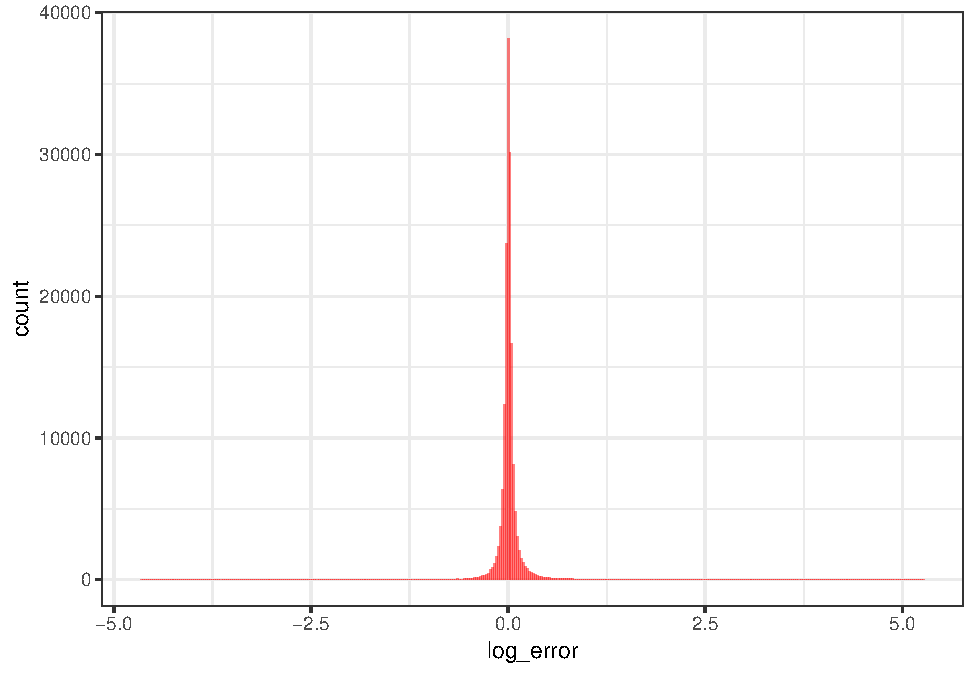
\includegraphics{zillow-prize_files/figure-latex/log-error-dist-all-1.pdf}
\caption{\label{fig:log-error-dist-all}Distribution of Log Error}
\end{figure}

\begin{Shaded}
\begin{Highlighting}[]
\NormalTok{trans }\OperatorTok\StringTok{ }
\StringTok{  }\KeywordTok{filter}\NormalTok{(}
\NormalTok{    log_error }\OperatorTok{>}\StringTok{ }\KeywordTok{quantile}\NormalTok{(log_error, }\DataTypeTok{probs =} \KeywordTok{c}\NormalTok{(.}\DecValTok{05}\NormalTok{)),}
\NormalTok{    log_error }\OperatorTok{<}\StringTok{ }\KeywordTok{quantile}\NormalTok{(log_error, }\DataTypeTok{probs =} \KeywordTok{c}\NormalTok{(.}\DecValTok{95}\NormalTok{))}
\NormalTok{  ) }\OperatorTok
\StringTok{  }\KeywordTok{ggplot}\NormalTok{(}\KeywordTok{aes}\NormalTok{(}\DataTypeTok{x =}\NormalTok{ log_error)) }\OperatorTok{+}\StringTok{ }
\StringTok{  }\KeywordTok{geom_histogram}\NormalTok{(}\DataTypeTok{fill =} \StringTok{"red"}\NormalTok{, }\DataTypeTok{alpha =} \FloatTok{0.5}\NormalTok{) }\OperatorTok{+}
\StringTok{  }\KeywordTok{theme_bw}\NormalTok{()}
\end{Highlighting}
\end{Shaded}

\begin{figure}
\centering
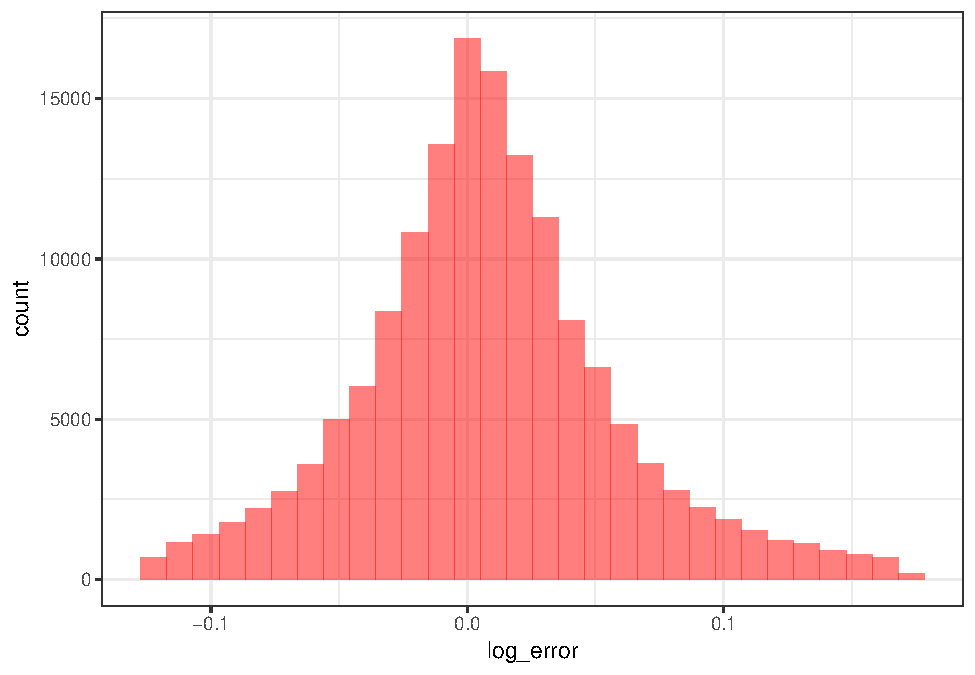
\includegraphics{zillow-prize_files/figure-latex/log-error-dist-95-1.pdf}
\caption{\label{fig:log-error-dist-95}Distribution of Log Error Between 5
and 95 Percentile}
\end{figure}

\begin{Shaded}
\begin{Highlighting}[]
\NormalTok{trans }\OperatorTok\StringTok{ }
\StringTok{  }\KeywordTok{filter}\NormalTok{(}
\NormalTok{    log_error }\OperatorTok{>}\StringTok{ }\KeywordTok{quantile}\NormalTok{(abs_log_error, }\DataTypeTok{probs =} \KeywordTok{c}\NormalTok{(.}\DecValTok{05}\NormalTok{)),}
\NormalTok{    log_error }\OperatorTok{<}\StringTok{ }\KeywordTok{quantile}\NormalTok{(abs_log_error, }\DataTypeTok{probs =} \KeywordTok{c}\NormalTok{(.}\DecValTok{95}\NormalTok{))}
\NormalTok{  ) }\OperatorTok
\StringTok{  }\KeywordTok{ggplot}\NormalTok{(}\KeywordTok{aes}\NormalTok{(}\DataTypeTok{x =}\NormalTok{ abs_log_error)) }\OperatorTok{+}\StringTok{ }
\StringTok{  }\KeywordTok{geom_histogram}\NormalTok{(}\DataTypeTok{fill =} \StringTok{"red"}\NormalTok{, }\DataTypeTok{alpha =} \FloatTok{0.5}\NormalTok{) }\OperatorTok{+}
\StringTok{  }\KeywordTok{theme_bw}\NormalTok{()}
\end{Highlighting}
\end{Shaded}

\begin{verbatim}
## `stat_bin()` using `bins = 30`. Pick better value with `binwidth`.
\end{verbatim}

\begin{figure}
\centering
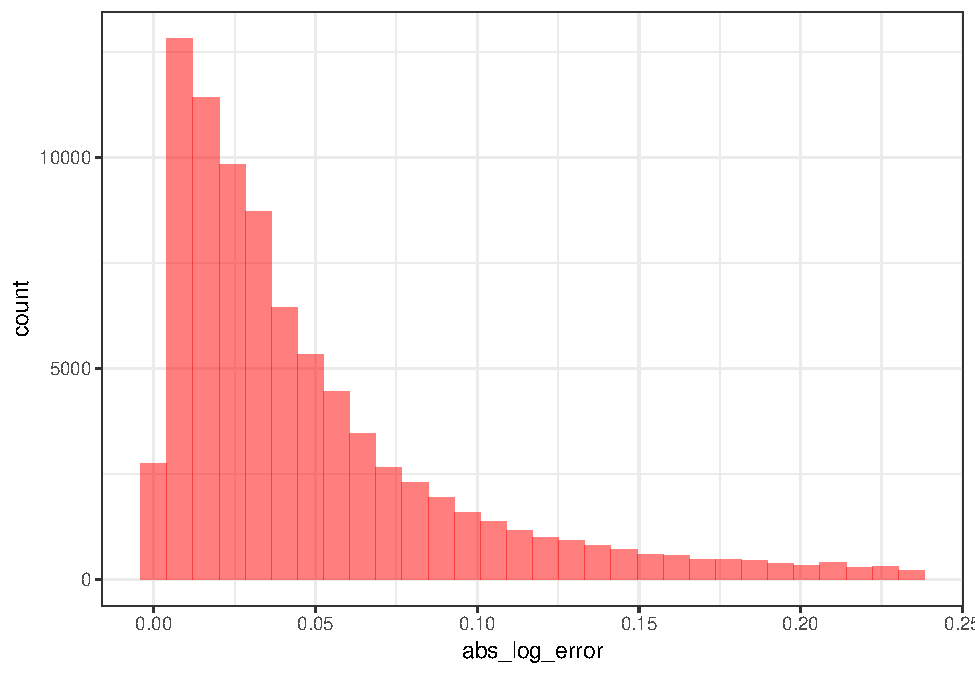
\includegraphics{zillow-prize_files/figure-latex/abs-log-error-dist-95-1.pdf}
\caption{\label{fig:abs-log-error-dist-95}Distribution of Absolute value of
Log Error Between 5 and 95 Percentile}
\end{figure}

\begin{Shaded}
\begin{Highlighting}[]
\NormalTok{trans }\OperatorTok\StringTok{ }
\StringTok{  }\KeywordTok{group_by}\NormalTok{(month_year) }\OperatorTok\StringTok{ }
\StringTok{  }\KeywordTok{summarise}\NormalTok{(}\DataTypeTok{mean_log_error =} \KeywordTok{mean}\NormalTok{(log_error)) }\OperatorTok\StringTok{ }
\StringTok{  }\KeywordTok{ggplot}\NormalTok{(}\KeywordTok{aes}\NormalTok{(}\DataTypeTok{x =}\NormalTok{ month_year, }\DataTypeTok{y =}\NormalTok{ mean_log_error)) }\OperatorTok{+}\StringTok{ }
\StringTok{  }\KeywordTok{geom_line}\NormalTok{(}\DataTypeTok{size =} \DecValTok{1}\NormalTok{, }\DataTypeTok{colour =} \StringTok{"red"}\NormalTok{) }\OperatorTok{+}
\StringTok{  }\KeywordTok{geom_point}\NormalTok{(}\DataTypeTok{size =} \DecValTok{3}\NormalTok{, }\DataTypeTok{colour =} \StringTok{"red"}\NormalTok{) }\OperatorTok{+}\StringTok{ }
\StringTok{  }\KeywordTok{theme_bw}\NormalTok{()}
\end{Highlighting}
\end{Shaded}

\begin{figure}
\centering
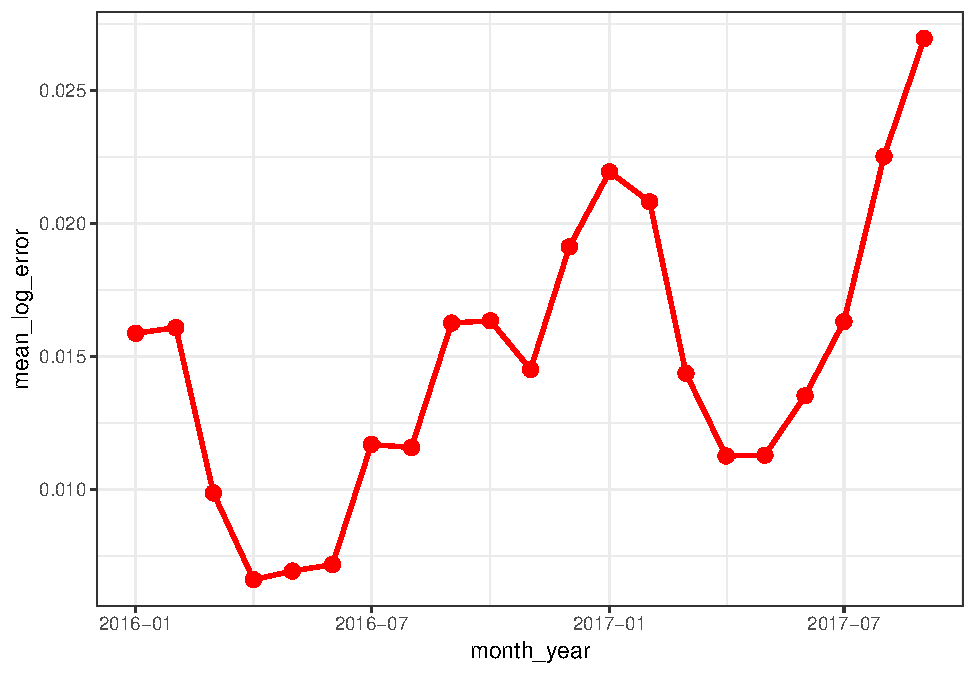
\includegraphics{zillow-prize_files/figure-latex/avg-le-by-month-1.pdf}
\caption{\label{fig:avg-le-by-month}Average Log Error by Month}
\end{figure}

\begin{Shaded}
\begin{Highlighting}[]
\NormalTok{trans }\OperatorTok\StringTok{ }
\StringTok{  }\KeywordTok{group_by}\NormalTok{(month_year, year, month) }\OperatorTok\StringTok{ }
\StringTok{  }\KeywordTok{summarise}\NormalTok{(}\DataTypeTok{mean_log_error =} \KeywordTok{mean}\NormalTok{(log_error)) }\OperatorTok\StringTok{  }
\StringTok{  }\KeywordTok{ungroup}\NormalTok{() }\OperatorTok
\StringTok{  }\KeywordTok{ggplot}\NormalTok{(}\KeywordTok{aes}\NormalTok{(}\DataTypeTok{x =} \KeywordTok{as.numeric}\NormalTok{(month), }\DataTypeTok{y =}\NormalTok{ mean_log_error)) }\OperatorTok{+}
\StringTok{  }\KeywordTok{geom_path}\NormalTok{(}\KeywordTok{aes}\NormalTok{(}\DataTypeTok{colour =} \KeywordTok{as.factor}\NormalTok{(year)), }\DataTypeTok{size =} \DecValTok{1}\NormalTok{) }\OperatorTok{+}
\StringTok{  }\KeywordTok{theme_bw}\NormalTok{() }\OperatorTok{+}
\StringTok{  }\KeywordTok{ylim}\NormalTok{(}\KeywordTok{c}\NormalTok{(}\DecValTok{0}\NormalTok{, .}\DecValTok{03}\NormalTok{)) }\OperatorTok{+}
\StringTok{  }\KeywordTok{scale_x_continuous}\NormalTok{(}\DataTypeTok{breaks =} \DecValTok{1}\OperatorTok{:}\DecValTok{12}\NormalTok{, }\DataTypeTok{labels =} \KeywordTok{levels}\NormalTok{(trans}\OperatorTok{$}\NormalTok{month)) }\OperatorTok{+}\StringTok{ }
\StringTok{  }\KeywordTok{labs}\NormalTok{(}
    \DataTypeTok{colour =} \OtherTok{NULL}\NormalTok{,}
    \DataTypeTok{x =} \StringTok{"month"}
\NormalTok{  )}
\end{Highlighting}
\end{Shaded}

\begin{figure}
\centering
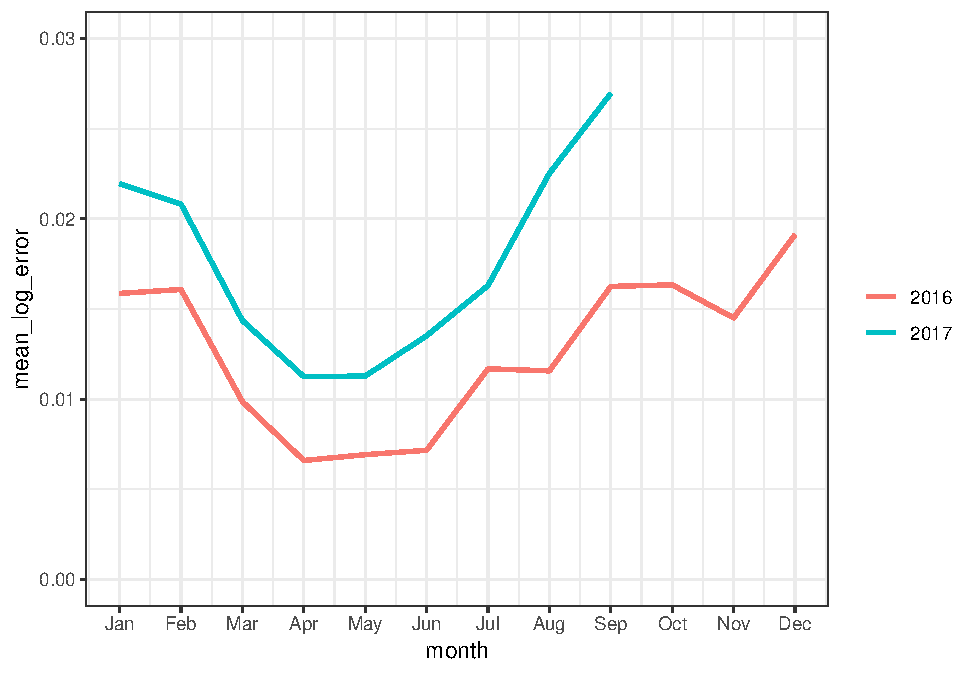
\includegraphics{zillow-prize_files/figure-latex/avg-le-by-month-year-1.pdf}
\caption{\label{fig:avg-le-by-month-year}Average Log Error by Month. 2017
Looks to have a higher baseline}
\end{figure}

\begin{Shaded}
\begin{Highlighting}[]
\NormalTok{trans }\OperatorTok
\StringTok{  }\KeywordTok{group_by}\NormalTok{(week_since_start) }\OperatorTok
\StringTok{  }\KeywordTok{summarise}\NormalTok{(}\DataTypeTok{mean_log_error =} \KeywordTok{mean}\NormalTok{(log_error)) }\OperatorTok
\StringTok{  }\KeywordTok{ggplot}\NormalTok{(}\KeywordTok{aes}\NormalTok{(}\DataTypeTok{x =}\NormalTok{ week_since_start, }\DataTypeTok{y =}\NormalTok{ mean_log_error)) }\OperatorTok{+}\StringTok{ }
\StringTok{  }\KeywordTok{geom_line}\NormalTok{(}\DataTypeTok{colour =} \StringTok{"red"}\NormalTok{, }\DataTypeTok{size =} \DecValTok{1}\NormalTok{) }\OperatorTok{+}
\StringTok{  }\KeywordTok{geom_smooth}\NormalTok{() }\OperatorTok{+}\StringTok{ }
\StringTok{  }\KeywordTok{theme_bw}\NormalTok{()}
\end{Highlighting}
\end{Shaded}

\begin{figure}
\centering
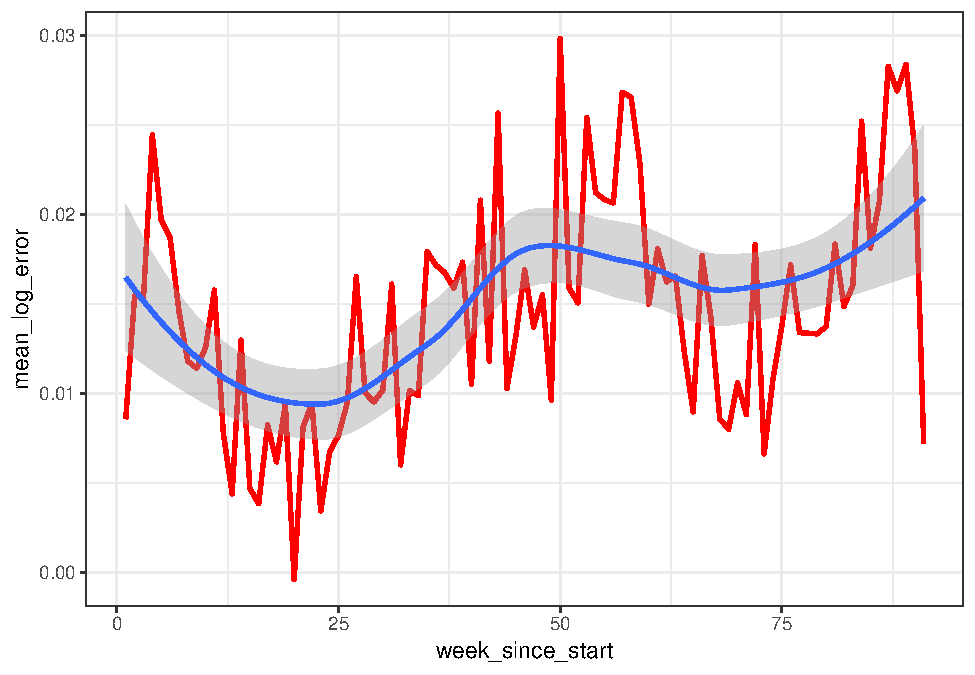
\includegraphics{zillow-prize_files/figure-latex/avg-le-by-week-1.pdf}
\caption{\label{fig:avg-le-by-week}Average Log Error by Week}
\end{figure}

\subsection{Transactions Over Time}\label{transactions-over-time}

\begin{Shaded}
\begin{Highlighting}[]
\NormalTok{trans }\OperatorTok\StringTok{ }
\StringTok{  }\KeywordTok{group_by}\NormalTok{(week_since_start) }\OperatorTok\StringTok{ }
\StringTok{  }\KeywordTok{summarise}\NormalTok{(}\DataTypeTok{n =} \KeywordTok{n}\NormalTok{()) }\OperatorTok\StringTok{ }
\StringTok{  }\KeywordTok{ggplot}\NormalTok{(}\KeywordTok{aes}\NormalTok{(}\DataTypeTok{x =}\NormalTok{ week_since_start, }\DataTypeTok{y =}\NormalTok{ n)) }\OperatorTok{+}
\StringTok{  }\KeywordTok{geom_line}\NormalTok{(}\DataTypeTok{colour =} \StringTok{"red"}\NormalTok{, }\DataTypeTok{size =} \DecValTok{1}\NormalTok{) }\OperatorTok{+}
\StringTok{  }\KeywordTok{theme_bw}\NormalTok{() }\OperatorTok{+}
\StringTok{  }\KeywordTok{labs}\NormalTok{(}
    \DataTypeTok{y =} \StringTok{"Numeber of Transactions"}
\NormalTok{  )}
\end{Highlighting}
\end{Shaded}

\begin{figure}
\centering
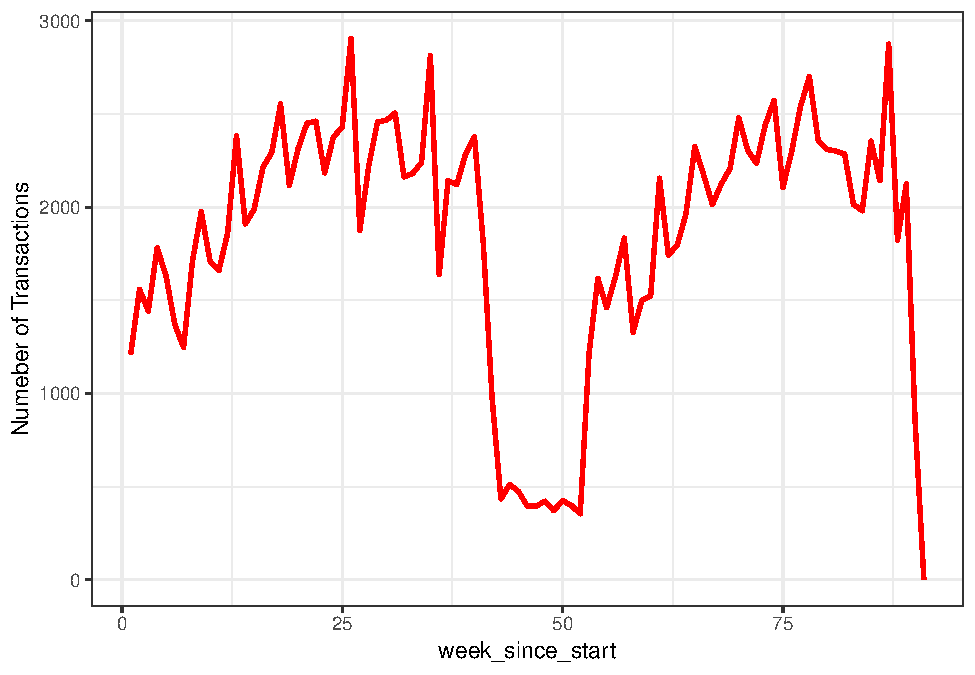
\includegraphics{zillow-prize_files/figure-latex/trans-per-week-1.pdf}
\caption{\label{fig:trans-per-week}Number of Transactions per Week. The dip
in the middle corresponds to the hold out testing data}
\end{figure}

\begin{Shaded}
\begin{Highlighting}[]
\NormalTok{trans }\OperatorTok\StringTok{ }
\StringTok{  }\KeywordTok{group_by}\NormalTok{(wday) }\OperatorTok\StringTok{ }
\StringTok{  }\KeywordTok{count}\NormalTok{() }\OperatorTok\StringTok{ }
\StringTok{  }\KeywordTok{ggplot}\NormalTok{(}\KeywordTok{aes}\NormalTok{(}\DataTypeTok{x =}\NormalTok{ wday, }\DataTypeTok{y =}\NormalTok{ n)) }\OperatorTok{+}
\StringTok{  }\KeywordTok{geom_bar}\NormalTok{(}\DataTypeTok{stat =} \StringTok{"identity"}\NormalTok{, }\DataTypeTok{fill =} \StringTok{"red"}\NormalTok{, }\DataTypeTok{alpha =} \FloatTok{0.5}\NormalTok{) }\OperatorTok{+}\StringTok{ }
\StringTok{  }\KeywordTok{theme_bw}\NormalTok{()}
\end{Highlighting}
\end{Shaded}

\begin{figure}
\centering
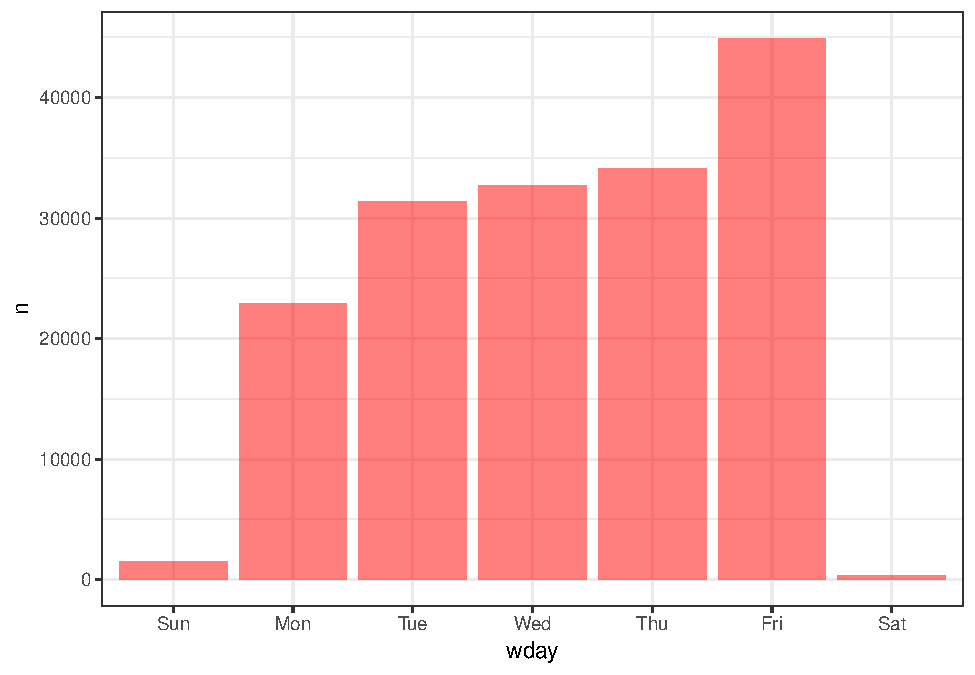
\includegraphics{zillow-prize_files/figure-latex/trans-by-wday-1.pdf}
\caption{\label{fig:trans-by-wday}Number of Transactions by Day of the
Week.}
\end{figure}

\subsection{\texorpdfstring{Spatial Distribution of
\texttt{log\_error}}{Spatial Distribution of log\_error}}\label{spatial-distribution-of-log_error}

\begin{Shaded}
\begin{Highlighting}[]
\KeywordTok{library}\NormalTok{(leaflet)}
\KeywordTok{library}\NormalTok{(leaflet.extras)}

\KeywordTok{read_feather}\NormalTok{(}\StringTok{"data/properties_geo_only.feather"}\NormalTok{) }\OperatorTok
\StringTok{  }\KeywordTok{right_join}\NormalTok{(trans, }\DataTypeTok{by =} \StringTok{"id_parcel"}\NormalTok{) }\OperatorTok
\StringTok{  }\KeywordTok{filter}\NormalTok{(}
    \OperatorTok{!}\KeywordTok{is.na}\NormalTok{(lat)}
\NormalTok{    ) }\OperatorTok
\KeywordTok{leaflet}\NormalTok{() }\OperatorTok\StringTok{ }
\StringTok{  }\KeywordTok{addProviderTiles}\NormalTok{(providers}\OperatorTok{$}\NormalTok{CartoDB.DarkMatter) }\OperatorTok
\StringTok{  }\KeywordTok{addHeatmap}\NormalTok{(}\DataTypeTok{lng=}\OperatorTok{~}\NormalTok{lon, }\DataTypeTok{lat=}\OperatorTok{~}\NormalTok{lat, }\DataTypeTok{intensity =} \OperatorTok{~}\NormalTok{log_error, }
             \DataTypeTok{radius =} \DecValTok{5}\NormalTok{, }\DataTypeTok{minOpacity =} \FloatTok{0.2}\NormalTok{, }\DataTypeTok{cellSize =} \DecValTok{6}\NormalTok{)}
\end{Highlighting}
\end{Shaded}

\begin{figure}
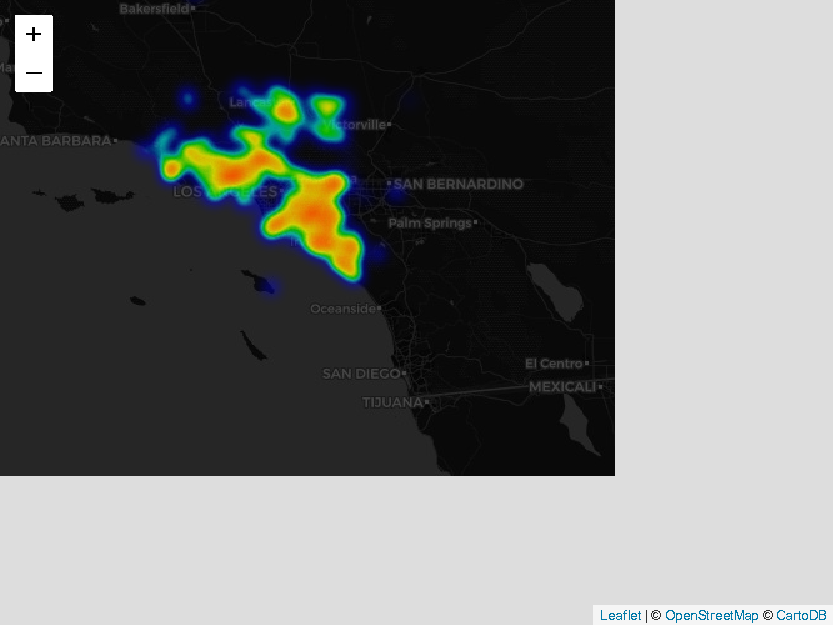
\includegraphics[width=1\linewidth]{zillow-prize_files/figure-latex/map-log-error-1} \caption{Spatial Distribution of Log Errors}\label{fig:map-log-error}
\end{figure}

\section{Predictor Variables}\label{predictor-variables}

Now lets take a look at the \texttt{properties} dataset. Based on the
descriptions from Kaggle, it seem's like the \texttt{properties\_17.csv}
has updated information and is a replacement from that of
\texttt{properties\_16.csv}. For our purposes we are only going to use
\texttt{properties\_17.csv}, however given more space, it would be
interesting to look into the differences in these files to see if there
were any patterns that could be useful.

\begin{Shaded}
\begin{Highlighting}[]
\NormalTok{properties <-}\StringTok{ }\KeywordTok{read_feather}\NormalTok{(}\StringTok{"data/properties_17.feather"}\NormalTok{)}
\end{Highlighting}
\end{Shaded}

Again apologies for the table formatting. Useful information none the
less.

\begin{Shaded}
\begin{Highlighting}[]
\KeywordTok{skim}\NormalTok{(properties) }\OperatorTok
\StringTok{  }\NormalTok{skimr}\OperatorTok{::}\KeywordTok{pander}\NormalTok{()}
\end{Highlighting}
\end{Shaded}

\begin{verbatim}
## Warning: Skimr's histograms incorrectly render with pander on Windows.
## Removing them. Use kable() if you'd like them rendered.
\end{verbatim}

Skim summary statistics\\
n obs: 2985217\\
n variables: 58

\begin{longtable}[]{@{}cccccccc@{}}
\toprule
\begin{minipage}[b]{0.23\columnwidth}\centering\strut
variable\strut
\end{minipage} & \begin{minipage}[b]{0.09\columnwidth}\centering\strut
missing\strut
\end{minipage} & \begin{minipage}[b]{0.10\columnwidth}\centering\strut
complete\strut
\end{minipage} & \begin{minipage}[b]{0.09\columnwidth}\centering\strut
n\strut
\end{minipage} & \begin{minipage}[b]{0.05\columnwidth}\centering\strut
min\strut
\end{minipage} & \begin{minipage}[b]{0.05\columnwidth}\centering\strut
max\strut
\end{minipage} & \begin{minipage}[b]{0.07\columnwidth}\centering\strut
empty\strut
\end{minipage} & \begin{minipage}[b]{0.09\columnwidth}\centering\strut
n\_unique\strut
\end{minipage}\tabularnewline
\midrule
\endhead
\begin{minipage}[t]{0.23\columnwidth}\centering\strut
fips\strut
\end{minipage} & \begin{minipage}[t]{0.09\columnwidth}\centering\strut
2932\strut
\end{minipage} & \begin{minipage}[t]{0.10\columnwidth}\centering\strut
2982285\strut
\end{minipage} & \begin{minipage}[t]{0.09\columnwidth}\centering\strut
2985217\strut
\end{minipage} & \begin{minipage}[t]{0.05\columnwidth}\centering\strut
5\strut
\end{minipage} & \begin{minipage}[t]{0.05\columnwidth}\centering\strut
5\strut
\end{minipage} & \begin{minipage}[t]{0.07\columnwidth}\centering\strut
0\strut
\end{minipage} & \begin{minipage}[t]{0.09\columnwidth}\centering\strut
3\strut
\end{minipage}\tabularnewline
\begin{minipage}[t]{0.23\columnwidth}\centering\strut
pooltypeid10\strut
\end{minipage} & \begin{minipage}[t]{0.09\columnwidth}\centering\strut
2968211\strut
\end{minipage} & \begin{minipage}[t]{0.10\columnwidth}\centering\strut
17006\strut
\end{minipage} & \begin{minipage}[t]{0.09\columnwidth}\centering\strut
2985217\strut
\end{minipage} & \begin{minipage}[t]{0.05\columnwidth}\centering\strut
1\strut
\end{minipage} & \begin{minipage}[t]{0.05\columnwidth}\centering\strut
1\strut
\end{minipage} & \begin{minipage}[t]{0.07\columnwidth}\centering\strut
0\strut
\end{minipage} & \begin{minipage}[t]{0.09\columnwidth}\centering\strut
1\strut
\end{minipage}\tabularnewline
\begin{minipage}[t]{0.23\columnwidth}\centering\strut
pooltypeid2\strut
\end{minipage} & \begin{minipage}[t]{0.09\columnwidth}\centering\strut
2952161\strut
\end{minipage} & \begin{minipage}[t]{0.10\columnwidth}\centering\strut
33056\strut
\end{minipage} & \begin{minipage}[t]{0.09\columnwidth}\centering\strut
2985217\strut
\end{minipage} & \begin{minipage}[t]{0.05\columnwidth}\centering\strut
1\strut
\end{minipage} & \begin{minipage}[t]{0.05\columnwidth}\centering\strut
1\strut
\end{minipage} & \begin{minipage}[t]{0.07\columnwidth}\centering\strut
0\strut
\end{minipage} & \begin{minipage}[t]{0.09\columnwidth}\centering\strut
1\strut
\end{minipage}\tabularnewline
\begin{minipage}[t]{0.23\columnwidth}\centering\strut
rawcensustractandblock\strut
\end{minipage} & \begin{minipage}[t]{0.09\columnwidth}\centering\strut
2932\strut
\end{minipage} & \begin{minipage}[t]{0.10\columnwidth}\centering\strut
2982285\strut
\end{minipage} & \begin{minipage}[t]{0.09\columnwidth}\centering\strut
2985217\strut
\end{minipage} & \begin{minipage}[t]{0.05\columnwidth}\centering\strut
12\strut
\end{minipage} & \begin{minipage}[t]{0.05\columnwidth}\centering\strut
16\strut
\end{minipage} & \begin{minipage}[t]{0.07\columnwidth}\centering\strut
0\strut
\end{minipage} & \begin{minipage}[t]{0.09\columnwidth}\centering\strut
100529\strut
\end{minipage}\tabularnewline
\begin{minipage}[t]{0.23\columnwidth}\centering\strut
str\_arch\_style\strut
\end{minipage} & \begin{minipage}[t]{0.09\columnwidth}\centering\strut
2979156\strut
\end{minipage} & \begin{minipage}[t]{0.10\columnwidth}\centering\strut
6061\strut
\end{minipage} & \begin{minipage}[t]{0.09\columnwidth}\centering\strut
2985217\strut
\end{minipage} & \begin{minipage}[t]{0.05\columnwidth}\centering\strut
1\strut
\end{minipage} & \begin{minipage}[t]{0.05\columnwidth}\centering\strut
2\strut
\end{minipage} & \begin{minipage}[t]{0.07\columnwidth}\centering\strut
0\strut
\end{minipage} & \begin{minipage}[t]{0.09\columnwidth}\centering\strut
8\strut
\end{minipage}\tabularnewline
\begin{minipage}[t]{0.23\columnwidth}\centering\strut
str\_material\strut
\end{minipage} & \begin{minipage}[t]{0.09\columnwidth}\centering\strut
2978471\strut
\end{minipage} & \begin{minipage}[t]{0.10\columnwidth}\centering\strut
6746\strut
\end{minipage} & \begin{minipage}[t]{0.09\columnwidth}\centering\strut
2985217\strut
\end{minipage} & \begin{minipage}[t]{0.05\columnwidth}\centering\strut
1\strut
\end{minipage} & \begin{minipage}[t]{0.05\columnwidth}\centering\strut
2\strut
\end{minipage} & \begin{minipage}[t]{0.07\columnwidth}\centering\strut
0\strut
\end{minipage} & \begin{minipage}[t]{0.09\columnwidth}\centering\strut
5\strut
\end{minipage}\tabularnewline
\begin{minipage}[t]{0.23\columnwidth}\centering\strut
zoning\_landuse\_county\strut
\end{minipage} & \begin{minipage}[t]{0.09\columnwidth}\centering\strut
2999\strut
\end{minipage} & \begin{minipage}[t]{0.10\columnwidth}\centering\strut
2982218\strut
\end{minipage} & \begin{minipage}[t]{0.09\columnwidth}\centering\strut
2985217\strut
\end{minipage} & \begin{minipage}[t]{0.05\columnwidth}\centering\strut
1\strut
\end{minipage} & \begin{minipage}[t]{0.05\columnwidth}\centering\strut
4\strut
\end{minipage} & \begin{minipage}[t]{0.07\columnwidth}\centering\strut
0\strut
\end{minipage} & \begin{minipage}[t]{0.09\columnwidth}\centering\strut
234\strut
\end{minipage}\tabularnewline
\begin{minipage}[t]{0.23\columnwidth}\centering\strut
zoning\_property\strut
\end{minipage} & \begin{minipage}[t]{0.09\columnwidth}\centering\strut
1002746\strut
\end{minipage} & \begin{minipage}[t]{0.10\columnwidth}\centering\strut
1982471\strut
\end{minipage} & \begin{minipage}[t]{0.09\columnwidth}\centering\strut
2985217\strut
\end{minipage} & \begin{minipage}[t]{0.05\columnwidth}\centering\strut
1\strut
\end{minipage} & \begin{minipage}[t]{0.05\columnwidth}\centering\strut
10\strut
\end{minipage} & \begin{minipage}[t]{0.07\columnwidth}\centering\strut
0\strut
\end{minipage} & \begin{minipage}[t]{0.09\columnwidth}\centering\strut
5651\strut
\end{minipage}\tabularnewline
\bottomrule
\end{longtable}

\begin{longtable}[]{@{}ccccc@{}}
\caption{Table continues below}\tabularnewline
\toprule
\begin{minipage}[b]{0.25\columnwidth}\centering\strut
variable\strut
\end{minipage} & \begin{minipage}[b]{0.12\columnwidth}\centering\strut
missing\strut
\end{minipage} & \begin{minipage}[b]{0.13\columnwidth}\centering\strut
complete\strut
\end{minipage} & \begin{minipage}[b]{0.12\columnwidth}\centering\strut
n\strut
\end{minipage} & \begin{minipage}[b]{0.12\columnwidth}\centering\strut
n\_unique\strut
\end{minipage}\tabularnewline
\midrule
\endfirsthead
\toprule
\begin{minipage}[b]{0.25\columnwidth}\centering\strut
variable\strut
\end{minipage} & \begin{minipage}[b]{0.12\columnwidth}\centering\strut
missing\strut
\end{minipage} & \begin{minipage}[b]{0.13\columnwidth}\centering\strut
complete\strut
\end{minipage} & \begin{minipage}[b]{0.12\columnwidth}\centering\strut
n\strut
\end{minipage} & \begin{minipage}[b]{0.12\columnwidth}\centering\strut
n\_unique\strut
\end{minipage}\tabularnewline
\midrule
\endhead
\begin{minipage}[t]{0.25\columnwidth}\centering\strut
str\_flag\_fireplace\strut
\end{minipage} & \begin{minipage}[t]{0.12\columnwidth}\centering\strut
2980054\strut
\end{minipage} & \begin{minipage}[t]{0.13\columnwidth}\centering\strut
5163\strut
\end{minipage} & \begin{minipage}[t]{0.12\columnwidth}\centering\strut
2985217\strut
\end{minipage} & \begin{minipage}[t]{0.12\columnwidth}\centering\strut
1\strut
\end{minipage}\tabularnewline
\begin{minipage}[t]{0.25\columnwidth}\centering\strut
str\_flag\_tub\strut
\end{minipage} & \begin{minipage}[t]{0.12\columnwidth}\centering\strut
2935155\strut
\end{minipage} & \begin{minipage}[t]{0.13\columnwidth}\centering\strut
50062\strut
\end{minipage} & \begin{minipage}[t]{0.12\columnwidth}\centering\strut
2985217\strut
\end{minipage} & \begin{minipage}[t]{0.12\columnwidth}\centering\strut
1\strut
\end{minipage}\tabularnewline
\begin{minipage}[t]{0.25\columnwidth}\centering\strut
tax\_delinquency\strut
\end{minipage} & \begin{minipage}[t]{0.12\columnwidth}\centering\strut
2928702\strut
\end{minipage} & \begin{minipage}[t]{0.13\columnwidth}\centering\strut
56515\strut
\end{minipage} & \begin{minipage}[t]{0.12\columnwidth}\centering\strut
2985217\strut
\end{minipage} & \begin{minipage}[t]{0.12\columnwidth}\centering\strut
1\strut
\end{minipage}\tabularnewline
\begin{minipage}[t]{0.25\columnwidth}\centering\strut
zoning\_landuse\strut
\end{minipage} & \begin{minipage}[t]{0.12\columnwidth}\centering\strut
2932\strut
\end{minipage} & \begin{minipage}[t]{0.13\columnwidth}\centering\strut
2982285\strut
\end{minipage} & \begin{minipage}[t]{0.12\columnwidth}\centering\strut
2985217\strut
\end{minipage} & \begin{minipage}[t]{0.12\columnwidth}\centering\strut
16\strut
\end{minipage}\tabularnewline
\bottomrule
\end{longtable}

\begin{longtable}[]{@{}cc@{}}
\toprule
\begin{minipage}[b]{0.38\columnwidth}\centering\strut
top\_counts\strut
\end{minipage} & \begin{minipage}[b]{0.12\columnwidth}\centering\strut
ordered\strut
\end{minipage}\tabularnewline
\midrule
\endhead
\begin{minipage}[t]{0.38\columnwidth}\centering\strut
NA: 2980054, No: 5163\strut
\end{minipage} & \begin{minipage}[t]{0.12\columnwidth}\centering\strut
FALSE\strut
\end{minipage}\tabularnewline
\begin{minipage}[t]{0.38\columnwidth}\centering\strut
NA: 2935155, No: 50062\strut
\end{minipage} & \begin{minipage}[t]{0.12\columnwidth}\centering\strut
FALSE\strut
\end{minipage}\tabularnewline
\begin{minipage}[t]{0.38\columnwidth}\centering\strut
NA: 2928702, Yes: 56515\strut
\end{minipage} & \begin{minipage}[t]{0.12\columnwidth}\centering\strut
FALSE\strut
\end{minipage}\tabularnewline
\begin{minipage}[t]{0.38\columnwidth}\centering\strut
Sin: 2152863, Con: 483789, Dup: 114415, Pla: 61559\strut
\end{minipage} & \begin{minipage}[t]{0.12\columnwidth}\centering\strut
FALSE\strut
\end{minipage}\tabularnewline
\bottomrule
\end{longtable}

\begin{longtable}[]{@{}ccccc@{}}
\caption{Table continues below}\tabularnewline
\toprule
\begin{minipage}[b]{0.35\columnwidth}\centering\strut
variable\strut
\end{minipage} & \begin{minipage}[b]{0.12\columnwidth}\centering\strut
missing\strut
\end{minipage} & \begin{minipage}[b]{0.13\columnwidth}\centering\strut
complete\strut
\end{minipage} & \begin{minipage}[b]{0.12\columnwidth}\centering\strut
n\strut
\end{minipage} & \begin{minipage}[b]{0.12\columnwidth}\centering\strut
mean\strut
\end{minipage}\tabularnewline
\midrule
\endfirsthead
\toprule
\begin{minipage}[b]{0.35\columnwidth}\centering\strut
variable\strut
\end{minipage} & \begin{minipage}[b]{0.12\columnwidth}\centering\strut
missing\strut
\end{minipage} & \begin{minipage}[b]{0.13\columnwidth}\centering\strut
complete\strut
\end{minipage} & \begin{minipage}[b]{0.12\columnwidth}\centering\strut
n\strut
\end{minipage} & \begin{minipage}[b]{0.12\columnwidth}\centering\strut
mean\strut
\end{minipage}\tabularnewline
\midrule
\endhead
\begin{minipage}[t]{0.35\columnwidth}\centering\strut
area\_base\strut
\end{minipage} & \begin{minipage}[t]{0.12\columnwidth}\centering\strut
2963735\strut
\end{minipage} & \begin{minipage}[t]{0.13\columnwidth}\centering\strut
21482\strut
\end{minipage} & \begin{minipage}[t]{0.12\columnwidth}\centering\strut
2985217\strut
\end{minipage} & \begin{minipage}[t]{0.12\columnwidth}\centering\strut
2427.56\strut
\end{minipage}\tabularnewline
\begin{minipage}[t]{0.35\columnwidth}\centering\strut
area\_basement\strut
\end{minipage} & \begin{minipage}[t]{0.12\columnwidth}\centering\strut
2983590\strut
\end{minipage} & \begin{minipage}[t]{0.13\columnwidth}\centering\strut
1627\strut
\end{minipage} & \begin{minipage}[t]{0.12\columnwidth}\centering\strut
2985217\strut
\end{minipage} & \begin{minipage}[t]{0.12\columnwidth}\centering\strut
647.22\strut
\end{minipage}\tabularnewline
\begin{minipage}[t]{0.35\columnwidth}\centering\strut
area\_firstfloor\_finished\_1\strut
\end{minipage} & \begin{minipage}[t]{0.12\columnwidth}\centering\strut
2781459\strut
\end{minipage} & \begin{minipage}[t]{0.13\columnwidth}\centering\strut
203758\strut
\end{minipage} & \begin{minipage}[t]{0.12\columnwidth}\centering\strut
2985217\strut
\end{minipage} & \begin{minipage}[t]{0.12\columnwidth}\centering\strut
1379.78\strut
\end{minipage}\tabularnewline
\begin{minipage}[t]{0.35\columnwidth}\centering\strut
area\_firstfloor\_finished\_2\strut
\end{minipage} & \begin{minipage}[t]{0.12\columnwidth}\centering\strut
2781459\strut
\end{minipage} & \begin{minipage}[t]{0.13\columnwidth}\centering\strut
203758\strut
\end{minipage} & \begin{minipage}[t]{0.12\columnwidth}\centering\strut
2985217\strut
\end{minipage} & \begin{minipage}[t]{0.12\columnwidth}\centering\strut
1392.03\strut
\end{minipage}\tabularnewline
\begin{minipage}[t]{0.35\columnwidth}\centering\strut
area\_garage\strut
\end{minipage} & \begin{minipage}[t]{0.12\columnwidth}\centering\strut
2094209\strut
\end{minipage} & \begin{minipage}[t]{0.13\columnwidth}\centering\strut
891008\strut
\end{minipage} & \begin{minipage}[t]{0.12\columnwidth}\centering\strut
2985217\strut
\end{minipage} & \begin{minipage}[t]{0.12\columnwidth}\centering\strut
383.16\strut
\end{minipage}\tabularnewline
\begin{minipage}[t]{0.35\columnwidth}\centering\strut
area\_living\_finished\strut
\end{minipage} & \begin{minipage}[t]{0.12\columnwidth}\centering\strut
264431\strut
\end{minipage} & \begin{minipage}[t]{0.13\columnwidth}\centering\strut
2720786\strut
\end{minipage} & \begin{minipage}[t]{0.12\columnwidth}\centering\strut
2985217\strut
\end{minipage} & \begin{minipage}[t]{0.12\columnwidth}\centering\strut
1764.04\strut
\end{minipage}\tabularnewline
\begin{minipage}[t]{0.35\columnwidth}\centering\strut
area\_living\_perimeter\strut
\end{minipage} & \begin{minipage}[t]{0.12\columnwidth}\centering\strut
2977546\strut
\end{minipage} & \begin{minipage}[t]{0.13\columnwidth}\centering\strut
7671\strut
\end{minipage} & \begin{minipage}[t]{0.12\columnwidth}\centering\strut
2985217\strut
\end{minipage} & \begin{minipage}[t]{0.12\columnwidth}\centering\strut
1178.92\strut
\end{minipage}\tabularnewline
\begin{minipage}[t]{0.35\columnwidth}\centering\strut
area\_patio\strut
\end{minipage} & \begin{minipage}[t]{0.12\columnwidth}\centering\strut
2903629\strut
\end{minipage} & \begin{minipage}[t]{0.13\columnwidth}\centering\strut
81588\strut
\end{minipage} & \begin{minipage}[t]{0.12\columnwidth}\centering\strut
2985217\strut
\end{minipage} & \begin{minipage}[t]{0.12\columnwidth}\centering\strut
321.54\strut
\end{minipage}\tabularnewline
\begin{minipage}[t]{0.35\columnwidth}\centering\strut
area\_pool\strut
\end{minipage} & \begin{minipage}[t]{0.12\columnwidth}\centering\strut
2957259\strut
\end{minipage} & \begin{minipage}[t]{0.13\columnwidth}\centering\strut
27958\strut
\end{minipage} & \begin{minipage}[t]{0.12\columnwidth}\centering\strut
2985217\strut
\end{minipage} & \begin{minipage}[t]{0.12\columnwidth}\centering\strut
519.72\strut
\end{minipage}\tabularnewline
\begin{minipage}[t]{0.35\columnwidth}\centering\strut
area\_shed\strut
\end{minipage} & \begin{minipage}[t]{0.12\columnwidth}\centering\strut
2982571\strut
\end{minipage} & \begin{minipage}[t]{0.13\columnwidth}\centering\strut
2646\strut
\end{minipage} & \begin{minipage}[t]{0.12\columnwidth}\centering\strut
2985217\strut
\end{minipage} & \begin{minipage}[t]{0.12\columnwidth}\centering\strut
278.37\strut
\end{minipage}\tabularnewline
\begin{minipage}[t]{0.35\columnwidth}\centering\strut
area\_total\strut
\end{minipage} & \begin{minipage}[t]{0.12\columnwidth}\centering\strut
2795032\strut
\end{minipage} & \begin{minipage}[t]{0.13\columnwidth}\centering\strut
190185\strut
\end{minipage} & \begin{minipage}[t]{0.12\columnwidth}\centering\strut
2985217\strut
\end{minipage} & \begin{minipage}[t]{0.12\columnwidth}\centering\strut
2754.87\strut
\end{minipage}\tabularnewline
\begin{minipage}[t]{0.35\columnwidth}\centering\strut
id\_parcel\strut
\end{minipage} & \begin{minipage}[t]{0.12\columnwidth}\centering\strut
0\strut
\end{minipage} & \begin{minipage}[t]{0.13\columnwidth}\centering\strut
2985217\strut
\end{minipage} & \begin{minipage}[t]{0.12\columnwidth}\centering\strut
2985217\strut
\end{minipage} & \begin{minipage}[t]{0.12\columnwidth}\centering\strut
1.3e+07\strut
\end{minipage}\tabularnewline
\begin{minipage}[t]{0.35\columnwidth}\centering\strut
latitude\strut
\end{minipage} & \begin{minipage}[t]{0.12\columnwidth}\centering\strut
2932\strut
\end{minipage} & \begin{minipage}[t]{0.13\columnwidth}\centering\strut
2982285\strut
\end{minipage} & \begin{minipage}[t]{0.12\columnwidth}\centering\strut
2985217\strut
\end{minipage} & \begin{minipage}[t]{0.12\columnwidth}\centering\strut
3.4e+07\strut
\end{minipage}\tabularnewline
\begin{minipage}[t]{0.35\columnwidth}\centering\strut
longitude\strut
\end{minipage} & \begin{minipage}[t]{0.12\columnwidth}\centering\strut
2932\strut
\end{minipage} & \begin{minipage}[t]{0.13\columnwidth}\centering\strut
2982285\strut
\end{minipage} & \begin{minipage}[t]{0.12\columnwidth}\centering\strut
2985217\strut
\end{minipage} & \begin{minipage}[t]{0.12\columnwidth}\centering\strut
-1.2e+08\strut
\end{minipage}\tabularnewline
\begin{minipage}[t]{0.35\columnwidth}\centering\strut
num\_75\_bath\strut
\end{minipage} & \begin{minipage}[t]{0.12\columnwidth}\centering\strut
2668860\strut
\end{minipage} & \begin{minipage}[t]{0.13\columnwidth}\centering\strut
316357\strut
\end{minipage} & \begin{minipage}[t]{0.12\columnwidth}\centering\strut
2985217\strut
\end{minipage} & \begin{minipage}[t]{0.12\columnwidth}\centering\strut
1.01\strut
\end{minipage}\tabularnewline
\begin{minipage}[t]{0.35\columnwidth}\centering\strut
num\_bath\strut
\end{minipage} & \begin{minipage}[t]{0.12\columnwidth}\centering\strut
117156\strut
\end{minipage} & \begin{minipage}[t]{0.13\columnwidth}\centering\strut
2868061\strut
\end{minipage} & \begin{minipage}[t]{0.12\columnwidth}\centering\strut
2985217\strut
\end{minipage} & \begin{minipage}[t]{0.12\columnwidth}\centering\strut
2.25\strut
\end{minipage}\tabularnewline
\begin{minipage}[t]{0.35\columnwidth}\centering\strut
num\_fireplace\strut
\end{minipage} & \begin{minipage}[t]{0.12\columnwidth}\centering\strut
2672093\strut
\end{minipage} & \begin{minipage}[t]{0.13\columnwidth}\centering\strut
313124\strut
\end{minipage} & \begin{minipage}[t]{0.12\columnwidth}\centering\strut
2985217\strut
\end{minipage} & \begin{minipage}[t]{0.12\columnwidth}\centering\strut
1.17\strut
\end{minipage}\tabularnewline
\begin{minipage}[t]{0.35\columnwidth}\centering\strut
num\_garage\strut
\end{minipage} & \begin{minipage}[t]{0.12\columnwidth}\centering\strut
2094209\strut
\end{minipage} & \begin{minipage}[t]{0.13\columnwidth}\centering\strut
891008\strut
\end{minipage} & \begin{minipage}[t]{0.12\columnwidth}\centering\strut
2985217\strut
\end{minipage} & \begin{minipage}[t]{0.12\columnwidth}\centering\strut
1.83\strut
\end{minipage}\tabularnewline
\begin{minipage}[t]{0.35\columnwidth}\centering\strut
num\_pool\strut
\end{minipage} & \begin{minipage}[t]{0.12\columnwidth}\centering\strut
2445585\strut
\end{minipage} & \begin{minipage}[t]{0.13\columnwidth}\centering\strut
539632\strut
\end{minipage} & \begin{minipage}[t]{0.12\columnwidth}\centering\strut
2985217\strut
\end{minipage} & \begin{minipage}[t]{0.12\columnwidth}\centering\strut
1\strut
\end{minipage}\tabularnewline
\begin{minipage}[t]{0.35\columnwidth}\centering\strut
num\_story\strut
\end{minipage} & \begin{minipage}[t]{0.12\columnwidth}\centering\strut
2299541\strut
\end{minipage} & \begin{minipage}[t]{0.13\columnwidth}\centering\strut
685676\strut
\end{minipage} & \begin{minipage}[t]{0.12\columnwidth}\centering\strut
2985217\strut
\end{minipage} & \begin{minipage}[t]{0.12\columnwidth}\centering\strut
1.4\strut
\end{minipage}\tabularnewline
\begin{minipage}[t]{0.35\columnwidth}\centering\strut
num\_unit\strut
\end{minipage} & \begin{minipage}[t]{0.12\columnwidth}\centering\strut
1004175\strut
\end{minipage} & \begin{minipage}[t]{0.13\columnwidth}\centering\strut
1981042\strut
\end{minipage} & \begin{minipage}[t]{0.12\columnwidth}\centering\strut
2985217\strut
\end{minipage} & \begin{minipage}[t]{0.12\columnwidth}\centering\strut
1.18\strut
\end{minipage}\tabularnewline
\begin{minipage}[t]{0.35\columnwidth}\centering\strut
pooltypeid7\strut
\end{minipage} & \begin{minipage}[t]{0.12\columnwidth}\centering\strut
2479322\strut
\end{minipage} & \begin{minipage}[t]{0.13\columnwidth}\centering\strut
505895\strut
\end{minipage} & \begin{minipage}[t]{0.12\columnwidth}\centering\strut
2985217\strut
\end{minipage} & \begin{minipage}[t]{0.12\columnwidth}\centering\strut
1\strut
\end{minipage}\tabularnewline
\begin{minipage}[t]{0.35\columnwidth}\centering\strut
region\_city\strut
\end{minipage} & \begin{minipage}[t]{0.12\columnwidth}\centering\strut
62128\strut
\end{minipage} & \begin{minipage}[t]{0.13\columnwidth}\centering\strut
2923089\strut
\end{minipage} & \begin{minipage}[t]{0.12\columnwidth}\centering\strut
2985217\strut
\end{minipage} & \begin{minipage}[t]{0.12\columnwidth}\centering\strut
34987.66\strut
\end{minipage}\tabularnewline
\begin{minipage}[t]{0.35\columnwidth}\centering\strut
region\_county\strut
\end{minipage} & \begin{minipage}[t]{0.12\columnwidth}\centering\strut
2932\strut
\end{minipage} & \begin{minipage}[t]{0.13\columnwidth}\centering\strut
2982285\strut
\end{minipage} & \begin{minipage}[t]{0.12\columnwidth}\centering\strut
2985217\strut
\end{minipage} & \begin{minipage}[t]{0.12\columnwidth}\centering\strut
2569.09\strut
\end{minipage}\tabularnewline
\begin{minipage}[t]{0.35\columnwidth}\centering\strut
region\_neighbor\strut
\end{minipage} & \begin{minipage}[t]{0.12\columnwidth}\centering\strut
1828476\strut
\end{minipage} & \begin{minipage}[t]{0.13\columnwidth}\centering\strut
1156741\strut
\end{minipage} & \begin{minipage}[t]{0.12\columnwidth}\centering\strut
2985217\strut
\end{minipage} & \begin{minipage}[t]{0.12\columnwidth}\centering\strut
193538.7\strut
\end{minipage}\tabularnewline
\begin{minipage}[t]{0.35\columnwidth}\centering\strut
region\_zip\strut
\end{minipage} & \begin{minipage}[t]{0.12\columnwidth}\centering\strut
12714\strut
\end{minipage} & \begin{minipage}[t]{0.13\columnwidth}\centering\strut
2972503\strut
\end{minipage} & \begin{minipage}[t]{0.12\columnwidth}\centering\strut
2985217\strut
\end{minipage} & \begin{minipage}[t]{0.12\columnwidth}\centering\strut
96553.29\strut
\end{minipage}\tabularnewline
\begin{minipage}[t]{0.35\columnwidth}\centering\strut
str\_aircon\strut
\end{minipage} & \begin{minipage}[t]{0.12\columnwidth}\centering\strut
2169855\strut
\end{minipage} & \begin{minipage}[t]{0.13\columnwidth}\centering\strut
815362\strut
\end{minipage} & \begin{minipage}[t]{0.12\columnwidth}\centering\strut
2985217\strut
\end{minipage} & \begin{minipage}[t]{0.12\columnwidth}\centering\strut
1.95\strut
\end{minipage}\tabularnewline
\begin{minipage}[t]{0.35\columnwidth}\centering\strut
str\_deck\strut
\end{minipage} & \begin{minipage}[t]{0.12\columnwidth}\centering\strut
2967838\strut
\end{minipage} & \begin{minipage}[t]{0.13\columnwidth}\centering\strut
17379\strut
\end{minipage} & \begin{minipage}[t]{0.12\columnwidth}\centering\strut
2985217\strut
\end{minipage} & \begin{minipage}[t]{0.12\columnwidth}\centering\strut
66\strut
\end{minipage}\tabularnewline
\begin{minipage}[t]{0.35\columnwidth}\centering\strut
str\_framing\strut
\end{minipage} & \begin{minipage}[t]{0.12\columnwidth}\centering\strut
2972486\strut
\end{minipage} & \begin{minipage}[t]{0.13\columnwidth}\centering\strut
12731\strut
\end{minipage} & \begin{minipage}[t]{0.12\columnwidth}\centering\strut
2985217\strut
\end{minipage} & \begin{minipage}[t]{0.12\columnwidth}\centering\strut
3.73\strut
\end{minipage}\tabularnewline
\begin{minipage}[t]{0.35\columnwidth}\centering\strut
str\_heating\strut
\end{minipage} & \begin{minipage}[t]{0.12\columnwidth}\centering\strut
1116053\strut
\end{minipage} & \begin{minipage}[t]{0.13\columnwidth}\centering\strut
1869164\strut
\end{minipage} & \begin{minipage}[t]{0.12\columnwidth}\centering\strut
2985217\strut
\end{minipage} & \begin{minipage}[t]{0.12\columnwidth}\centering\strut
4.08\strut
\end{minipage}\tabularnewline
\begin{minipage}[t]{0.35\columnwidth}\centering\strut
str\_quality\strut
\end{minipage} & \begin{minipage}[t]{0.12\columnwidth}\centering\strut
1043822\strut
\end{minipage} & \begin{minipage}[t]{0.13\columnwidth}\centering\strut
1941395\strut
\end{minipage} & \begin{minipage}[t]{0.12\columnwidth}\centering\strut
2985217\strut
\end{minipage} & \begin{minipage}[t]{0.12\columnwidth}\centering\strut
6.28\strut
\end{minipage}\tabularnewline
\begin{minipage}[t]{0.35\columnwidth}\centering\strut
str\_story\strut
\end{minipage} & \begin{minipage}[t]{0.12\columnwidth}\centering\strut
2983594\strut
\end{minipage} & \begin{minipage}[t]{0.13\columnwidth}\centering\strut
1623\strut
\end{minipage} & \begin{minipage}[t]{0.12\columnwidth}\centering\strut
2985217\strut
\end{minipage} & \begin{minipage}[t]{0.12\columnwidth}\centering\strut
7\strut
\end{minipage}\tabularnewline
\begin{minipage}[t]{0.35\columnwidth}\centering\strut
tax\_delinquency\_year\strut
\end{minipage} & \begin{minipage}[t]{0.12\columnwidth}\centering\strut
2928700\strut
\end{minipage} & \begin{minipage}[t]{0.13\columnwidth}\centering\strut
56517\strut
\end{minipage} & \begin{minipage}[t]{0.12\columnwidth}\centering\strut
2985217\strut
\end{minipage} & \begin{minipage}[t]{0.12\columnwidth}\centering\strut
13.89\strut
\end{minipage}\tabularnewline
\begin{minipage}[t]{0.35\columnwidth}\centering\strut
tax\_year\strut
\end{minipage} & \begin{minipage}[t]{0.12\columnwidth}\centering\strut
2933\strut
\end{minipage} & \begin{minipage}[t]{0.13\columnwidth}\centering\strut
2982284\strut
\end{minipage} & \begin{minipage}[t]{0.12\columnwidth}\centering\strut
2985217\strut
\end{minipage} & \begin{minipage}[t]{0.12\columnwidth}\centering\strut
2016\strut
\end{minipage}\tabularnewline
\bottomrule
\end{longtable}

\begin{longtable}[]{@{}cccccc@{}}
\toprule
\begin{minipage}[b]{0.15\columnwidth}\centering\strut
sd\strut
\end{minipage} & \begin{minipage}[b]{0.13\columnwidth}\centering\strut
p0\strut
\end{minipage} & \begin{minipage}[b]{0.13\columnwidth}\centering\strut
p25\strut
\end{minipage} & \begin{minipage}[b]{0.13\columnwidth}\centering\strut
p50\strut
\end{minipage} & \begin{minipage}[b]{0.13\columnwidth}\centering\strut
p75\strut
\end{minipage} & \begin{minipage}[b]{0.13\columnwidth}\centering\strut
p100\strut
\end{minipage}\tabularnewline
\midrule
\endhead
\begin{minipage}[t]{0.15\columnwidth}\centering\strut
7786.19\strut
\end{minipage} & \begin{minipage}[t]{0.13\columnwidth}\centering\strut
117\strut
\end{minipage} & \begin{minipage}[t]{0.13\columnwidth}\centering\strut
1072\strut
\end{minipage} & \begin{minipage}[t]{0.13\columnwidth}\centering\strut
2008\strut
\end{minipage} & \begin{minipage}[t]{0.13\columnwidth}\centering\strut
3411\strut
\end{minipage} & \begin{minipage}[t]{0.13\columnwidth}\centering\strut
952576\strut
\end{minipage}\tabularnewline
\begin{minipage}[t]{0.15\columnwidth}\centering\strut
538.79\strut
\end{minipage} & \begin{minipage}[t]{0.13\columnwidth}\centering\strut
20\strut
\end{minipage} & \begin{minipage}[t]{0.13\columnwidth}\centering\strut
272\strut
\end{minipage} & \begin{minipage}[t]{0.13\columnwidth}\centering\strut
535\strut
\end{minipage} & \begin{minipage}[t]{0.13\columnwidth}\centering\strut
847.5\strut
\end{minipage} & \begin{minipage}[t]{0.13\columnwidth}\centering\strut
8516\strut
\end{minipage}\tabularnewline
\begin{minipage}[t]{0.15\columnwidth}\centering\strut
634.42\strut
\end{minipage} & \begin{minipage}[t]{0.13\columnwidth}\centering\strut
1\strut
\end{minipage} & \begin{minipage}[t]{0.13\columnwidth}\centering\strut
1010\strut
\end{minipage} & \begin{minipage}[t]{0.13\columnwidth}\centering\strut
1281\strut
\end{minipage} & \begin{minipage}[t]{0.13\columnwidth}\centering\strut
1615\strut
\end{minipage} & \begin{minipage}[t]{0.13\columnwidth}\centering\strut
31303\strut
\end{minipage}\tabularnewline
\begin{minipage}[t]{0.15\columnwidth}\centering\strut
682.32\strut
\end{minipage} & \begin{minipage}[t]{0.13\columnwidth}\centering\strut
3\strut
\end{minipage} & \begin{minipage}[t]{0.13\columnwidth}\centering\strut
1012\strut
\end{minipage} & \begin{minipage}[t]{0.13\columnwidth}\centering\strut
1284\strut
\end{minipage} & \begin{minipage}[t]{0.13\columnwidth}\centering\strut
1619\strut
\end{minipage} & \begin{minipage}[t]{0.13\columnwidth}\centering\strut
41906\strut
\end{minipage}\tabularnewline
\begin{minipage}[t]{0.15\columnwidth}\centering\strut
246.22\strut
\end{minipage} & \begin{minipage}[t]{0.13\columnwidth}\centering\strut
0\strut
\end{minipage} & \begin{minipage}[t]{0.13\columnwidth}\centering\strut
312\strut
\end{minipage} & \begin{minipage}[t]{0.13\columnwidth}\centering\strut
441\strut
\end{minipage} & \begin{minipage}[t]{0.13\columnwidth}\centering\strut
494\strut
\end{minipage} & \begin{minipage}[t]{0.13\columnwidth}\centering\strut
7749\strut
\end{minipage}\tabularnewline
\begin{minipage}[t]{0.15\columnwidth}\centering\strut
1031.38\strut
\end{minipage} & \begin{minipage}[t]{0.13\columnwidth}\centering\strut
1\strut
\end{minipage} & \begin{minipage}[t]{0.13\columnwidth}\centering\strut
1198\strut
\end{minipage} & \begin{minipage}[t]{0.13\columnwidth}\centering\strut
1542\strut
\end{minipage} & \begin{minipage}[t]{0.13\columnwidth}\centering\strut
2075\strut
\end{minipage} & \begin{minipage}[t]{0.13\columnwidth}\centering\strut
427079\strut
\end{minipage}\tabularnewline
\begin{minipage}[t]{0.15\columnwidth}\centering\strut
357.09\strut
\end{minipage} & \begin{minipage}[t]{0.13\columnwidth}\centering\strut
120\strut
\end{minipage} & \begin{minipage}[t]{0.13\columnwidth}\centering\strut
960\strut
\end{minipage} & \begin{minipage}[t]{0.13\columnwidth}\centering\strut
1296\strut
\end{minipage} & \begin{minipage}[t]{0.13\columnwidth}\centering\strut
1440\strut
\end{minipage} & \begin{minipage}[t]{0.13\columnwidth}\centering\strut
2688\strut
\end{minipage}\tabularnewline
\begin{minipage}[t]{0.15\columnwidth}\centering\strut
236.88\strut
\end{minipage} & \begin{minipage}[t]{0.13\columnwidth}\centering\strut
10\strut
\end{minipage} & \begin{minipage}[t]{0.13\columnwidth}\centering\strut
190\strut
\end{minipage} & \begin{minipage}[t]{0.13\columnwidth}\centering\strut
270\strut
\end{minipage} & \begin{minipage}[t]{0.13\columnwidth}\centering\strut
390\strut
\end{minipage} & \begin{minipage}[t]{0.13\columnwidth}\centering\strut
7983\strut
\end{minipage}\tabularnewline
\begin{minipage}[t]{0.15\columnwidth}\centering\strut
191.33\strut
\end{minipage} & \begin{minipage}[t]{0.13\columnwidth}\centering\strut
19\strut
\end{minipage} & \begin{minipage}[t]{0.13\columnwidth}\centering\strut
430\strut
\end{minipage} & \begin{minipage}[t]{0.13\columnwidth}\centering\strut
495\strut
\end{minipage} & \begin{minipage}[t]{0.13\columnwidth}\centering\strut
594\strut
\end{minipage} & \begin{minipage}[t]{0.13\columnwidth}\centering\strut
17410\strut
\end{minipage}\tabularnewline
\begin{minipage}[t]{0.15\columnwidth}\centering\strut
369.78\strut
\end{minipage} & \begin{minipage}[t]{0.13\columnwidth}\centering\strut
10\strut
\end{minipage} & \begin{minipage}[t]{0.13\columnwidth}\centering\strut
96\strut
\end{minipage} & \begin{minipage}[t]{0.13\columnwidth}\centering\strut
168\strut
\end{minipage} & \begin{minipage}[t]{0.13\columnwidth}\centering\strut
320\strut
\end{minipage} & \begin{minipage}[t]{0.13\columnwidth}\centering\strut
6141\strut
\end{minipage}\tabularnewline
\begin{minipage}[t]{0.15\columnwidth}\centering\strut
5999.38\strut
\end{minipage} & \begin{minipage}[t]{0.13\columnwidth}\centering\strut
112\strut
\end{minipage} & \begin{minipage}[t]{0.13\columnwidth}\centering\strut
1696\strut
\end{minipage} & \begin{minipage}[t]{0.13\columnwidth}\centering\strut
2173\strut
\end{minipage} & \begin{minipage}[t]{0.13\columnwidth}\centering\strut
2975\strut
\end{minipage} & \begin{minipage}[t]{0.13\columnwidth}\centering\strut
820242\strut
\end{minipage}\tabularnewline
\begin{minipage}[t]{0.15\columnwidth}\centering\strut
7909966.39\strut
\end{minipage} & \begin{minipage}[t]{0.13\columnwidth}\centering\strut
1.1e+07\strut
\end{minipage} & \begin{minipage}[t]{0.13\columnwidth}\centering\strut
1.2e+07\strut
\end{minipage} & \begin{minipage}[t]{0.13\columnwidth}\centering\strut
1.3e+07\strut
\end{minipage} & \begin{minipage}[t]{0.13\columnwidth}\centering\strut
1.4e+07\strut
\end{minipage} & \begin{minipage}[t]{0.13\columnwidth}\centering\strut
1.7e+08\strut
\end{minipage}\tabularnewline
\begin{minipage}[t]{0.15\columnwidth}\centering\strut
243515.71\strut
\end{minipage} & \begin{minipage}[t]{0.13\columnwidth}\centering\strut
3.3e+07\strut
\end{minipage} & \begin{minipage}[t]{0.13\columnwidth}\centering\strut
3.4e+07\strut
\end{minipage} & \begin{minipage}[t]{0.13\columnwidth}\centering\strut
3.4e+07\strut
\end{minipage} & \begin{minipage}[t]{0.13\columnwidth}\centering\strut
3.4e+07\strut
\end{minipage} & \begin{minipage}[t]{0.13\columnwidth}\centering\strut
3.5e+07\strut
\end{minipage}\tabularnewline
\begin{minipage}[t]{0.15\columnwidth}\centering\strut
345591.77\strut
\end{minipage} & \begin{minipage}[t]{0.13\columnwidth}\centering\strut
-1.2e+08\strut
\end{minipage} & \begin{minipage}[t]{0.13\columnwidth}\centering\strut
-1.2e+08\strut
\end{minipage} & \begin{minipage}[t]{0.13\columnwidth}\centering\strut
-1.2e+08\strut
\end{minipage} & \begin{minipage}[t]{0.13\columnwidth}\centering\strut
-1.2e+08\strut
\end{minipage} & \begin{minipage}[t]{0.13\columnwidth}\centering\strut
-1.2e+08\strut
\end{minipage}\tabularnewline
\begin{minipage}[t]{0.15\columnwidth}\centering\strut
0.12\strut
\end{minipage} & \begin{minipage}[t]{0.13\columnwidth}\centering\strut
1\strut
\end{minipage} & \begin{minipage}[t]{0.13\columnwidth}\centering\strut
1\strut
\end{minipage} & \begin{minipage}[t]{0.13\columnwidth}\centering\strut
1\strut
\end{minipage} & \begin{minipage}[t]{0.13\columnwidth}\centering\strut
1\strut
\end{minipage} & \begin{minipage}[t]{0.13\columnwidth}\centering\strut
7\strut
\end{minipage}\tabularnewline
\begin{minipage}[t]{0.15\columnwidth}\centering\strut
0.99\strut
\end{minipage} & \begin{minipage}[t]{0.13\columnwidth}\centering\strut
1\strut
\end{minipage} & \begin{minipage}[t]{0.13\columnwidth}\centering\strut
2\strut
\end{minipage} & \begin{minipage}[t]{0.13\columnwidth}\centering\strut
2\strut
\end{minipage} & \begin{minipage}[t]{0.13\columnwidth}\centering\strut
3\strut
\end{minipage} & \begin{minipage}[t]{0.13\columnwidth}\centering\strut
32\strut
\end{minipage}\tabularnewline
\begin{minipage}[t]{0.15\columnwidth}\centering\strut
0.46\strut
\end{minipage} & \begin{minipage}[t]{0.13\columnwidth}\centering\strut
1\strut
\end{minipage} & \begin{minipage}[t]{0.13\columnwidth}\centering\strut
1\strut
\end{minipage} & \begin{minipage}[t]{0.13\columnwidth}\centering\strut
1\strut
\end{minipage} & \begin{minipage}[t]{0.13\columnwidth}\centering\strut
1\strut
\end{minipage} & \begin{minipage}[t]{0.13\columnwidth}\centering\strut
9\strut
\end{minipage}\tabularnewline
\begin{minipage}[t]{0.15\columnwidth}\centering\strut
0.61\strut
\end{minipage} & \begin{minipage}[t]{0.13\columnwidth}\centering\strut
0\strut
\end{minipage} & \begin{minipage}[t]{0.13\columnwidth}\centering\strut
2\strut
\end{minipage} & \begin{minipage}[t]{0.13\columnwidth}\centering\strut
2\strut
\end{minipage} & \begin{minipage}[t]{0.13\columnwidth}\centering\strut
2\strut
\end{minipage} & \begin{minipage}[t]{0.13\columnwidth}\centering\strut
25\strut
\end{minipage}\tabularnewline
\begin{minipage}[t]{0.15\columnwidth}\centering\strut
0\strut
\end{minipage} & \begin{minipage}[t]{0.13\columnwidth}\centering\strut
1\strut
\end{minipage} & \begin{minipage}[t]{0.13\columnwidth}\centering\strut
1\strut
\end{minipage} & \begin{minipage}[t]{0.13\columnwidth}\centering\strut
1\strut
\end{minipage} & \begin{minipage}[t]{0.13\columnwidth}\centering\strut
1\strut
\end{minipage} & \begin{minipage}[t]{0.13\columnwidth}\centering\strut
1\strut
\end{minipage}\tabularnewline
\begin{minipage}[t]{0.15\columnwidth}\centering\strut
0.54\strut
\end{minipage} & \begin{minipage}[t]{0.13\columnwidth}\centering\strut
1\strut
\end{minipage} & \begin{minipage}[t]{0.13\columnwidth}\centering\strut
1\strut
\end{minipage} & \begin{minipage}[t]{0.13\columnwidth}\centering\strut
1\strut
\end{minipage} & \begin{minipage}[t]{0.13\columnwidth}\centering\strut
2\strut
\end{minipage} & \begin{minipage}[t]{0.13\columnwidth}\centering\strut
41\strut
\end{minipage}\tabularnewline
\begin{minipage}[t]{0.15\columnwidth}\centering\strut
2.49\strut
\end{minipage} & \begin{minipage}[t]{0.13\columnwidth}\centering\strut
1\strut
\end{minipage} & \begin{minipage}[t]{0.13\columnwidth}\centering\strut
1\strut
\end{minipage} & \begin{minipage}[t]{0.13\columnwidth}\centering\strut
1\strut
\end{minipage} & \begin{minipage}[t]{0.13\columnwidth}\centering\strut
1\strut
\end{minipage} & \begin{minipage}[t]{0.13\columnwidth}\centering\strut
997\strut
\end{minipage}\tabularnewline
\begin{minipage}[t]{0.15\columnwidth}\centering\strut
0\strut
\end{minipage} & \begin{minipage}[t]{0.13\columnwidth}\centering\strut
1\strut
\end{minipage} & \begin{minipage}[t]{0.13\columnwidth}\centering\strut
1\strut
\end{minipage} & \begin{minipage}[t]{0.13\columnwidth}\centering\strut
1\strut
\end{minipage} & \begin{minipage}[t]{0.13\columnwidth}\centering\strut
1\strut
\end{minipage} & \begin{minipage}[t]{0.13\columnwidth}\centering\strut
1\strut
\end{minipage}\tabularnewline
\begin{minipage}[t]{0.15\columnwidth}\centering\strut
50709.68\strut
\end{minipage} & \begin{minipage}[t]{0.13\columnwidth}\centering\strut
3491\strut
\end{minipage} & \begin{minipage}[t]{0.13\columnwidth}\centering\strut
12447\strut
\end{minipage} & \begin{minipage}[t]{0.13\columnwidth}\centering\strut
25218\strut
\end{minipage} & \begin{minipage}[t]{0.13\columnwidth}\centering\strut
45457\strut
\end{minipage} & \begin{minipage}[t]{0.13\columnwidth}\centering\strut
4e+05\strut
\end{minipage}\tabularnewline
\begin{minipage}[t]{0.15\columnwidth}\centering\strut
788.68\strut
\end{minipage} & \begin{minipage}[t]{0.13\columnwidth}\centering\strut
1286\strut
\end{minipage} & \begin{minipage}[t]{0.13\columnwidth}\centering\strut
1286\strut
\end{minipage} & \begin{minipage}[t]{0.13\columnwidth}\centering\strut
3101\strut
\end{minipage} & \begin{minipage}[t]{0.13\columnwidth}\centering\strut
3101\strut
\end{minipage} & \begin{minipage}[t]{0.13\columnwidth}\centering\strut
3101\strut
\end{minipage}\tabularnewline
\begin{minipage}[t]{0.15\columnwidth}\centering\strut
165725.27\strut
\end{minipage} & \begin{minipage}[t]{0.13\columnwidth}\centering\strut
6952\strut
\end{minipage} & \begin{minipage}[t]{0.13\columnwidth}\centering\strut
46736\strut
\end{minipage} & \begin{minipage}[t]{0.13\columnwidth}\centering\strut
118920\strut
\end{minipage} & \begin{minipage}[t]{0.13\columnwidth}\centering\strut
274800\strut
\end{minipage} & \begin{minipage}[t]{0.13\columnwidth}\centering\strut
764167\strut
\end{minipage}\tabularnewline
\begin{minipage}[t]{0.15\columnwidth}\centering\strut
3680.82\strut
\end{minipage} & \begin{minipage}[t]{0.13\columnwidth}\centering\strut
95982\strut
\end{minipage} & \begin{minipage}[t]{0.13\columnwidth}\centering\strut
96180\strut
\end{minipage} & \begin{minipage}[t]{0.13\columnwidth}\centering\strut
96377\strut
\end{minipage} & \begin{minipage}[t]{0.13\columnwidth}\centering\strut
96974\strut
\end{minipage} & \begin{minipage}[t]{0.13\columnwidth}\centering\strut
4e+05\strut
\end{minipage}\tabularnewline
\begin{minipage}[t]{0.15\columnwidth}\centering\strut
3.16\strut
\end{minipage} & \begin{minipage}[t]{0.13\columnwidth}\centering\strut
1\strut
\end{minipage} & \begin{minipage}[t]{0.13\columnwidth}\centering\strut
1\strut
\end{minipage} & \begin{minipage}[t]{0.13\columnwidth}\centering\strut
1\strut
\end{minipage} & \begin{minipage}[t]{0.13\columnwidth}\centering\strut
1\strut
\end{minipage} & \begin{minipage}[t]{0.13\columnwidth}\centering\strut
13\strut
\end{minipage}\tabularnewline
\begin{minipage}[t]{0.15\columnwidth}\centering\strut
0\strut
\end{minipage} & \begin{minipage}[t]{0.13\columnwidth}\centering\strut
66\strut
\end{minipage} & \begin{minipage}[t]{0.13\columnwidth}\centering\strut
66\strut
\end{minipage} & \begin{minipage}[t]{0.13\columnwidth}\centering\strut
66\strut
\end{minipage} & \begin{minipage}[t]{0.13\columnwidth}\centering\strut
66\strut
\end{minipage} & \begin{minipage}[t]{0.13\columnwidth}\centering\strut
66\strut
\end{minipage}\tabularnewline
\begin{minipage}[t]{0.15\columnwidth}\centering\strut
0.5\strut
\end{minipage} & \begin{minipage}[t]{0.13\columnwidth}\centering\strut
1\strut
\end{minipage} & \begin{minipage}[t]{0.13\columnwidth}\centering\strut
3\strut
\end{minipage} & \begin{minipage}[t]{0.13\columnwidth}\centering\strut
4\strut
\end{minipage} & \begin{minipage}[t]{0.13\columnwidth}\centering\strut
4\strut
\end{minipage} & \begin{minipage}[t]{0.13\columnwidth}\centering\strut
5\strut
\end{minipage}\tabularnewline
\begin{minipage}[t]{0.15\columnwidth}\centering\strut
3.29\strut
\end{minipage} & \begin{minipage}[t]{0.13\columnwidth}\centering\strut
1\strut
\end{minipage} & \begin{minipage}[t]{0.13\columnwidth}\centering\strut
2\strut
\end{minipage} & \begin{minipage}[t]{0.13\columnwidth}\centering\strut
2\strut
\end{minipage} & \begin{minipage}[t]{0.13\columnwidth}\centering\strut
7\strut
\end{minipage} & \begin{minipage}[t]{0.13\columnwidth}\centering\strut
24\strut
\end{minipage}\tabularnewline
\begin{minipage}[t]{0.15\columnwidth}\centering\strut
1.73\strut
\end{minipage} & \begin{minipage}[t]{0.13\columnwidth}\centering\strut
1\strut
\end{minipage} & \begin{minipage}[t]{0.13\columnwidth}\centering\strut
5\strut
\end{minipage} & \begin{minipage}[t]{0.13\columnwidth}\centering\strut
6\strut
\end{minipage} & \begin{minipage}[t]{0.13\columnwidth}\centering\strut
8\strut
\end{minipage} & \begin{minipage}[t]{0.13\columnwidth}\centering\strut
12\strut
\end{minipage}\tabularnewline
\begin{minipage}[t]{0.15\columnwidth}\centering\strut
0\strut
\end{minipage} & \begin{minipage}[t]{0.13\columnwidth}\centering\strut
7\strut
\end{minipage} & \begin{minipage}[t]{0.13\columnwidth}\centering\strut
7\strut
\end{minipage} & \begin{minipage}[t]{0.13\columnwidth}\centering\strut
7\strut
\end{minipage} & \begin{minipage}[t]{0.13\columnwidth}\centering\strut
7\strut
\end{minipage} & \begin{minipage}[t]{0.13\columnwidth}\centering\strut
7\strut
\end{minipage}\tabularnewline
\begin{minipage}[t]{0.15\columnwidth}\centering\strut
2.56\strut
\end{minipage} & \begin{minipage}[t]{0.13\columnwidth}\centering\strut
0\strut
\end{minipage} & \begin{minipage}[t]{0.13\columnwidth}\centering\strut
14\strut
\end{minipage} & \begin{minipage}[t]{0.13\columnwidth}\centering\strut
14\strut
\end{minipage} & \begin{minipage}[t]{0.13\columnwidth}\centering\strut
15\strut
\end{minipage} & \begin{minipage}[t]{0.13\columnwidth}\centering\strut
99\strut
\end{minipage}\tabularnewline
\begin{minipage}[t]{0.15\columnwidth}\centering\strut
0.06\strut
\end{minipage} & \begin{minipage}[t]{0.13\columnwidth}\centering\strut
2000\strut
\end{minipage} & \begin{minipage}[t]{0.13\columnwidth}\centering\strut
2016\strut
\end{minipage} & \begin{minipage}[t]{0.13\columnwidth}\centering\strut
2016\strut
\end{minipage} & \begin{minipage}[t]{0.13\columnwidth}\centering\strut
2016\strut
\end{minipage} & \begin{minipage}[t]{0.13\columnwidth}\centering\strut
2016\strut
\end{minipage}\tabularnewline
\bottomrule
\end{longtable}

\begin{longtable}[]{@{}ccccc@{}}
\caption{Table continues below}\tabularnewline
\toprule
\begin{minipage}[b]{0.33\columnwidth}\centering\strut
variable\strut
\end{minipage} & \begin{minipage}[b]{0.12\columnwidth}\centering\strut
missing\strut
\end{minipage} & \begin{minipage}[b]{0.13\columnwidth}\centering\strut
complete\strut
\end{minipage} & \begin{minipage}[b]{0.12\columnwidth}\centering\strut
n\strut
\end{minipage} & \begin{minipage}[b]{0.13\columnwidth}\centering\strut
mean\strut
\end{minipage}\tabularnewline
\midrule
\endfirsthead
\toprule
\begin{minipage}[b]{0.33\columnwidth}\centering\strut
variable\strut
\end{minipage} & \begin{minipage}[b]{0.12\columnwidth}\centering\strut
missing\strut
\end{minipage} & \begin{minipage}[b]{0.13\columnwidth}\centering\strut
complete\strut
\end{minipage} & \begin{minipage}[b]{0.12\columnwidth}\centering\strut
n\strut
\end{minipage} & \begin{minipage}[b]{0.13\columnwidth}\centering\strut
mean\strut
\end{minipage}\tabularnewline
\midrule
\endhead
\begin{minipage}[t]{0.33\columnwidth}\centering\strut
area\_living\_finished\_calc\strut
\end{minipage} & \begin{minipage}[t]{0.12\columnwidth}\centering\strut
45097\strut
\end{minipage} & \begin{minipage}[t]{0.13\columnwidth}\centering\strut
2940120\strut
\end{minipage} & \begin{minipage}[t]{0.12\columnwidth}\centering\strut
2985217\strut
\end{minipage} & \begin{minipage}[t]{0.13\columnwidth}\centering\strut
1831.46\strut
\end{minipage}\tabularnewline
\begin{minipage}[t]{0.33\columnwidth}\centering\strut
area\_lot\strut
\end{minipage} & \begin{minipage}[t]{0.12\columnwidth}\centering\strut
272706\strut
\end{minipage} & \begin{minipage}[t]{0.13\columnwidth}\centering\strut
2712511\strut
\end{minipage} & \begin{minipage}[t]{0.12\columnwidth}\centering\strut
2985217\strut
\end{minipage} & \begin{minipage}[t]{0.13\columnwidth}\centering\strut
22603.76\strut
\end{minipage}\tabularnewline
\begin{minipage}[t]{0.33\columnwidth}\centering\strut
build\_year\strut
\end{minipage} & \begin{minipage}[t]{0.12\columnwidth}\centering\strut
47833\strut
\end{minipage} & \begin{minipage}[t]{0.13\columnwidth}\centering\strut
2937384\strut
\end{minipage} & \begin{minipage}[t]{0.12\columnwidth}\centering\strut
2985217\strut
\end{minipage} & \begin{minipage}[t]{0.13\columnwidth}\centering\strut
1964.44\strut
\end{minipage}\tabularnewline
\begin{minipage}[t]{0.33\columnwidth}\centering\strut
censustractandblock\strut
\end{minipage} & \begin{minipage}[t]{0.12\columnwidth}\centering\strut
74985\strut
\end{minipage} & \begin{minipage}[t]{0.13\columnwidth}\centering\strut
2910232\strut
\end{minipage} & \begin{minipage}[t]{0.12\columnwidth}\centering\strut
2985217\strut
\end{minipage} & \begin{minipage}[t]{0.13\columnwidth}\centering\strut
6e+13\strut
\end{minipage}\tabularnewline
\begin{minipage}[t]{0.33\columnwidth}\centering\strut
num\_bathroom\strut
\end{minipage} & \begin{minipage}[t]{0.12\columnwidth}\centering\strut
2957\strut
\end{minipage} & \begin{minipage}[t]{0.13\columnwidth}\centering\strut
2982260\strut
\end{minipage} & \begin{minipage}[t]{0.12\columnwidth}\centering\strut
2985217\strut
\end{minipage} & \begin{minipage}[t]{0.13\columnwidth}\centering\strut
2.22\strut
\end{minipage}\tabularnewline
\begin{minipage}[t]{0.33\columnwidth}\centering\strut
num\_bathroom\_calc\strut
\end{minipage} & \begin{minipage}[t]{0.12\columnwidth}\centering\strut
117156\strut
\end{minipage} & \begin{minipage}[t]{0.13\columnwidth}\centering\strut
2868061\strut
\end{minipage} & \begin{minipage}[t]{0.12\columnwidth}\centering\strut
2985217\strut
\end{minipage} & \begin{minipage}[t]{0.13\columnwidth}\centering\strut
2.3\strut
\end{minipage}\tabularnewline
\begin{minipage}[t]{0.33\columnwidth}\centering\strut
num\_bedroom\strut
\end{minipage} & \begin{minipage}[t]{0.12\columnwidth}\centering\strut
2945\strut
\end{minipage} & \begin{minipage}[t]{0.13\columnwidth}\centering\strut
2982272\strut
\end{minipage} & \begin{minipage}[t]{0.12\columnwidth}\centering\strut
2985217\strut
\end{minipage} & \begin{minipage}[t]{0.13\columnwidth}\centering\strut
3.09\strut
\end{minipage}\tabularnewline
\begin{minipage}[t]{0.33\columnwidth}\centering\strut
num\_room\strut
\end{minipage} & \begin{minipage}[t]{0.12\columnwidth}\centering\strut
2969\strut
\end{minipage} & \begin{minipage}[t]{0.13\columnwidth}\centering\strut
2982248\strut
\end{minipage} & \begin{minipage}[t]{0.12\columnwidth}\centering\strut
2985217\strut
\end{minipage} & \begin{minipage}[t]{0.13\columnwidth}\centering\strut
1.47\strut
\end{minipage}\tabularnewline
\begin{minipage}[t]{0.33\columnwidth}\centering\strut
tax\_building\strut
\end{minipage} & \begin{minipage}[t]{0.12\columnwidth}\centering\strut
46464\strut
\end{minipage} & \begin{minipage}[t]{0.13\columnwidth}\centering\strut
2938753\strut
\end{minipage} & \begin{minipage}[t]{0.12\columnwidth}\centering\strut
2985217\strut
\end{minipage} & \begin{minipage}[t]{0.13\columnwidth}\centering\strut
178142.89\strut
\end{minipage}\tabularnewline
\begin{minipage}[t]{0.33\columnwidth}\centering\strut
tax\_land\strut
\end{minipage} & \begin{minipage}[t]{0.12\columnwidth}\centering\strut
59926\strut
\end{minipage} & \begin{minipage}[t]{0.13\columnwidth}\centering\strut
2925291\strut
\end{minipage} & \begin{minipage}[t]{0.12\columnwidth}\centering\strut
2985217\strut
\end{minipage} & \begin{minipage}[t]{0.13\columnwidth}\centering\strut
268455.77\strut
\end{minipage}\tabularnewline
\begin{minipage}[t]{0.33\columnwidth}\centering\strut
tax\_property\strut
\end{minipage} & \begin{minipage}[t]{0.12\columnwidth}\centering\strut
22752\strut
\end{minipage} & \begin{minipage}[t]{0.13\columnwidth}\centering\strut
2962465\strut
\end{minipage} & \begin{minipage}[t]{0.12\columnwidth}\centering\strut
2985217\strut
\end{minipage} & \begin{minipage}[t]{0.13\columnwidth}\centering\strut
5408.95\strut
\end{minipage}\tabularnewline
\begin{minipage}[t]{0.33\columnwidth}\centering\strut
tax\_total\strut
\end{minipage} & \begin{minipage}[t]{0.12\columnwidth}\centering\strut
34266\strut
\end{minipage} & \begin{minipage}[t]{0.13\columnwidth}\centering\strut
2950951\strut
\end{minipage} & \begin{minipage}[t]{0.12\columnwidth}\centering\strut
2985217\strut
\end{minipage} & \begin{minipage}[t]{0.13\columnwidth}\centering\strut
443527.93\strut
\end{minipage}\tabularnewline
\bottomrule
\end{longtable}

\begin{longtable}[]{@{}cccccc@{}}
\toprule
\begin{minipage}[b]{0.14\columnwidth}\centering\strut
sd\strut
\end{minipage} & \begin{minipage}[b]{0.08\columnwidth}\centering\strut
p0\strut
\end{minipage} & \begin{minipage}[b]{0.12\columnwidth}\centering\strut
p25\strut
\end{minipage} & \begin{minipage}[b]{0.12\columnwidth}\centering\strut
p50\strut
\end{minipage} & \begin{minipage}[b]{0.12\columnwidth}\centering\strut
p75\strut
\end{minipage} & \begin{minipage}[b]{0.14\columnwidth}\centering\strut
p100\strut
\end{minipage}\tabularnewline
\midrule
\endhead
\begin{minipage}[t]{0.14\columnwidth}\centering\strut
1954.2\strut
\end{minipage} & \begin{minipage}[t]{0.08\columnwidth}\centering\strut
1\strut
\end{minipage} & \begin{minipage}[t]{0.12\columnwidth}\centering\strut
1215\strut
\end{minipage} & \begin{minipage}[t]{0.12\columnwidth}\centering\strut
1574\strut
\end{minipage} & \begin{minipage}[t]{0.12\columnwidth}\centering\strut
2140\strut
\end{minipage} & \begin{minipage}[t]{0.14\columnwidth}\centering\strut
952576\strut
\end{minipage}\tabularnewline
\begin{minipage}[t]{0.14\columnwidth}\centering\strut
249983.63\strut
\end{minipage} & \begin{minipage}[t]{0.08\columnwidth}\centering\strut
100\strut
\end{minipage} & \begin{minipage}[t]{0.12\columnwidth}\centering\strut
5683\strut
\end{minipage} & \begin{minipage}[t]{0.12\columnwidth}\centering\strut
7000\strut
\end{minipage} & \begin{minipage}[t]{0.12\columnwidth}\centering\strut
9893\strut
\end{minipage} & \begin{minipage}[t]{0.14\columnwidth}\centering\strut
3.7e+08\strut
\end{minipage}\tabularnewline
\begin{minipage}[t]{0.14\columnwidth}\centering\strut
23.64\strut
\end{minipage} & \begin{minipage}[t]{0.08\columnwidth}\centering\strut
1801\strut
\end{minipage} & \begin{minipage}[t]{0.12\columnwidth}\centering\strut
1950\strut
\end{minipage} & \begin{minipage}[t]{0.12\columnwidth}\centering\strut
1963\strut
\end{minipage} & \begin{minipage}[t]{0.12\columnwidth}\centering\strut
1981\strut
\end{minipage} & \begin{minipage}[t]{0.14\columnwidth}\centering\strut
2016\strut
\end{minipage}\tabularnewline
\begin{minipage}[t]{0.14\columnwidth}\centering\strut
3.2e+11\strut
\end{minipage} & \begin{minipage}[t]{0.08\columnwidth}\centering\strut
-1\strut
\end{minipage} & \begin{minipage}[t]{0.12\columnwidth}\centering\strut
6e+13\strut
\end{minipage} & \begin{minipage}[t]{0.12\columnwidth}\centering\strut
6e+13\strut
\end{minipage} & \begin{minipage}[t]{0.12\columnwidth}\centering\strut
6.1e+13\strut
\end{minipage} & \begin{minipage}[t]{0.14\columnwidth}\centering\strut
4.8e+14\strut
\end{minipage}\tabularnewline
\begin{minipage}[t]{0.14\columnwidth}\centering\strut
1.08\strut
\end{minipage} & \begin{minipage}[t]{0.08\columnwidth}\centering\strut
0\strut
\end{minipage} & \begin{minipage}[t]{0.12\columnwidth}\centering\strut
2\strut
\end{minipage} & \begin{minipage}[t]{0.12\columnwidth}\centering\strut
2\strut
\end{minipage} & \begin{minipage}[t]{0.12\columnwidth}\centering\strut
3\strut
\end{minipage} & \begin{minipage}[t]{0.14\columnwidth}\centering\strut
32\strut
\end{minipage}\tabularnewline
\begin{minipage}[t]{0.14\columnwidth}\centering\strut
1\strut
\end{minipage} & \begin{minipage}[t]{0.08\columnwidth}\centering\strut
1\strut
\end{minipage} & \begin{minipage}[t]{0.12\columnwidth}\centering\strut
2\strut
\end{minipage} & \begin{minipage}[t]{0.12\columnwidth}\centering\strut
2\strut
\end{minipage} & \begin{minipage}[t]{0.12\columnwidth}\centering\strut
3\strut
\end{minipage} & \begin{minipage}[t]{0.14\columnwidth}\centering\strut
32\strut
\end{minipage}\tabularnewline
\begin{minipage}[t]{0.14\columnwidth}\centering\strut
1.27\strut
\end{minipage} & \begin{minipage}[t]{0.08\columnwidth}\centering\strut
0\strut
\end{minipage} & \begin{minipage}[t]{0.12\columnwidth}\centering\strut
2\strut
\end{minipage} & \begin{minipage}[t]{0.12\columnwidth}\centering\strut
3\strut
\end{minipage} & \begin{minipage}[t]{0.12\columnwidth}\centering\strut
4\strut
\end{minipage} & \begin{minipage}[t]{0.14\columnwidth}\centering\strut
25\strut
\end{minipage}\tabularnewline
\begin{minipage}[t]{0.14\columnwidth}\centering\strut
2.84\strut
\end{minipage} & \begin{minipage}[t]{0.08\columnwidth}\centering\strut
0\strut
\end{minipage} & \begin{minipage}[t]{0.12\columnwidth}\centering\strut
0\strut
\end{minipage} & \begin{minipage}[t]{0.12\columnwidth}\centering\strut
0\strut
\end{minipage} & \begin{minipage}[t]{0.12\columnwidth}\centering\strut
0\strut
\end{minipage} & \begin{minipage}[t]{0.14\columnwidth}\centering\strut
96\strut
\end{minipage}\tabularnewline
\begin{minipage}[t]{0.14\columnwidth}\centering\strut
460050.31\strut
\end{minipage} & \begin{minipage}[t]{0.08\columnwidth}\centering\strut
1\strut
\end{minipage} & \begin{minipage}[t]{0.12\columnwidth}\centering\strut
77666\strut
\end{minipage} & \begin{minipage}[t]{0.12\columnwidth}\centering\strut
127066\strut
\end{minipage} & \begin{minipage}[t]{0.12\columnwidth}\centering\strut
2e+05\strut
\end{minipage} & \begin{minipage}[t]{0.14\columnwidth}\centering\strut
2.6e+08\strut
\end{minipage}\tabularnewline
\begin{minipage}[t]{0.14\columnwidth}\centering\strut
486509.71\strut
\end{minipage} & \begin{minipage}[t]{0.08\columnwidth}\centering\strut
1\strut
\end{minipage} & \begin{minipage}[t]{0.12\columnwidth}\centering\strut
79700\strut
\end{minipage} & \begin{minipage}[t]{0.12\columnwidth}\centering\strut
176619\strut
\end{minipage} & \begin{minipage}[t]{0.12\columnwidth}\centering\strut
326100\strut
\end{minipage} & \begin{minipage}[t]{0.14\columnwidth}\centering\strut
9.4e+07\strut
\end{minipage}\tabularnewline
\begin{minipage}[t]{0.14\columnwidth}\centering\strut
9675.57\strut
\end{minipage} & \begin{minipage}[t]{0.08\columnwidth}\centering\strut
0.24\strut
\end{minipage} & \begin{minipage}[t]{0.12\columnwidth}\centering\strut
2468.62\strut
\end{minipage} & \begin{minipage}[t]{0.12\columnwidth}\centering\strut
4007.62\strut
\end{minipage} & \begin{minipage}[t]{0.12\columnwidth}\centering\strut
6230.5\strut
\end{minipage} & \begin{minipage}[t]{0.14\columnwidth}\centering\strut
3823175.65\strut
\end{minipage}\tabularnewline
\begin{minipage}[t]{0.14\columnwidth}\centering\strut
816336.63\strut
\end{minipage} & \begin{minipage}[t]{0.08\columnwidth}\centering\strut
1\strut
\end{minipage} & \begin{minipage}[t]{0.12\columnwidth}\centering\strut
188220\strut
\end{minipage} & \begin{minipage}[t]{0.12\columnwidth}\centering\strut
321161\strut
\end{minipage} & \begin{minipage}[t]{0.12\columnwidth}\centering\strut
514072\strut
\end{minipage} & \begin{minipage}[t]{0.14\columnwidth}\centering\strut
3.2e+08\strut
\end{minipage}\tabularnewline
\bottomrule
\end{longtable}

\subsection{Missingness}\label{missingness}

Missing values in data is a cold cruel reality. It is one of the most
contraining factors there is when it comes to predictive power. Having a
good understanding of the prevalence of missing values and any patterns
to them is needed to make the most out of what data you do have.

\begin{Shaded}
\begin{Highlighting}[]
\NormalTok{missing_data <-}\StringTok{ }\KeywordTok{plot_missing}\NormalTok{(properties, }\DataTypeTok{theme =} \KeywordTok{theme_bw}\NormalTok{())}
\end{Highlighting}
\end{Shaded}

\begin{figure}
\centering
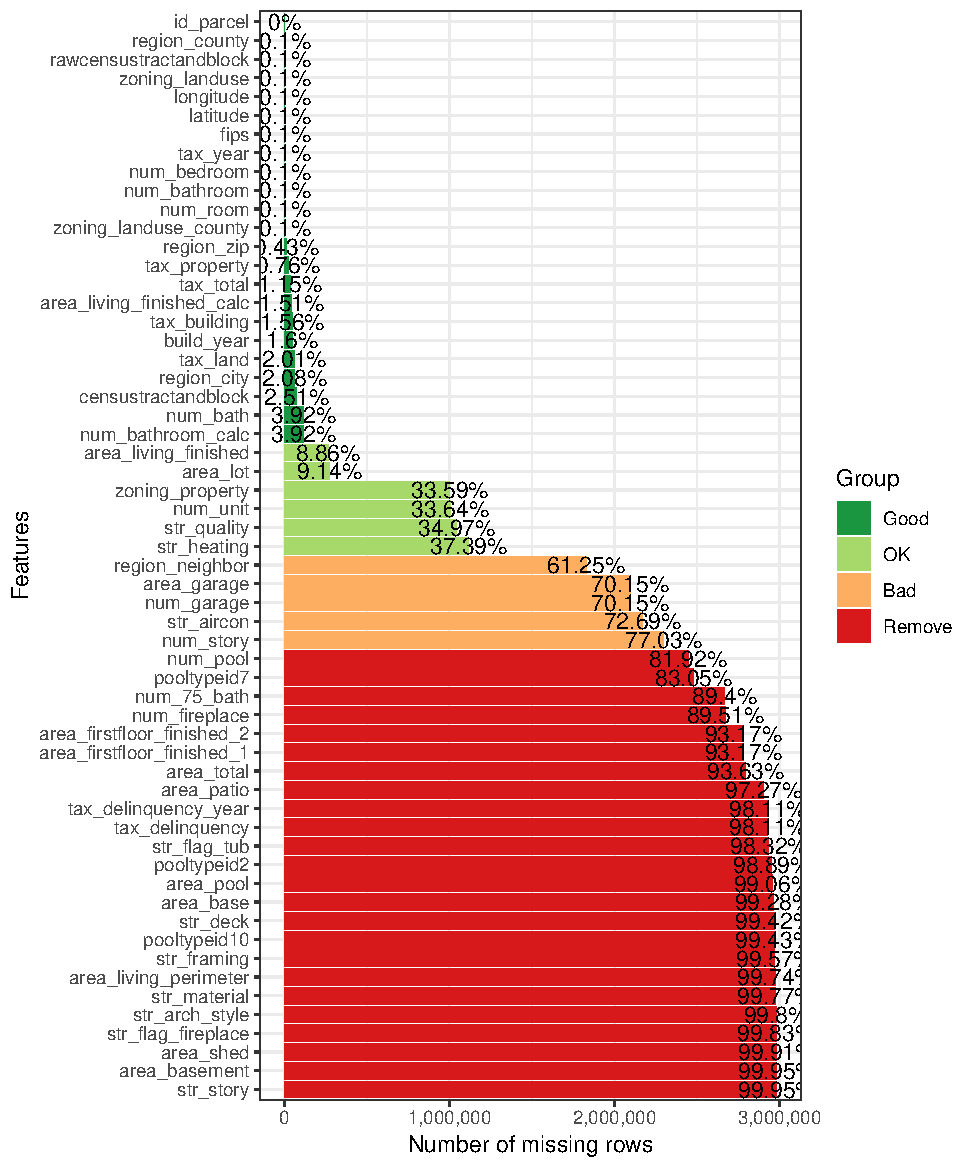
\includegraphics{zillow-prize_files/figure-latex/miss-plot-1.pdf}
\caption{\label{fig:miss-plot}Completeness by Feature. Many are extremely
sparse}
\end{figure}

\begin{Shaded}
\begin{Highlighting}[]
\NormalTok{missing_data}
\end{Highlighting}
\end{Shaded}

\begin{verbatim}
## # A tibble: 58 x 4
##    feature           num_missing pct_missing group 
##    <fct>                   <int>       <dbl> <chr> 
##  1 id_parcel                   0    0        Good  
##  2 str_aircon            2169855    0.727    Bad   
##  3 str_arch_style        2979156    0.998    Remove
##  4 area_basement         2983590    0.999    Remove
##  5 num_bathroom             2957    0.000991 Good  
##  6 num_bedroom              2945    0.000987 Good  
##  7 str_framing           2972486    0.996    Remove
##  8 str_quality           1043822    0.350    OK    
##  9 num_bathroom_calc      117156    0.0392   Good  
## 10 str_deck              2967838    0.994    Remove
## # ... with 48 more rows
\end{verbatim}

There seem to be quite a lot of missing features. For now lets remove
the ones that are over 50\% missing and continue on with those that are
more than 50\% complete. We could come back to the ones we dropped and
try to recover some of those missing values with more sophisticated
methods, for example we could impute the missing values based on their
spatial neighbors but for now we will continue with the ones that have
over 50\% of their values.

A few of the features, \texttt{rawcensustractandblock}, \texttt{fips},
and \texttt{censustractandblock}, and \texttt{region\_county} are ID
fields for their census geography units. Since we have already extracted
that information earlier in \texttt{properties\_geo} we will drop them
here as well since we can add the information contained in those
features in a cleaner format later.

Additionally, based on the descriptions, \texttt{zoning\_landuse},
\texttt{zoning\_landuse\_county}, and \texttt{zoning\_property} all seem
to contain pretty similar information.Since the number of unique
categories are fairly large for each one, if they are redundant they
could add needless complexity and computation time to our model. Let's
use a chi-squared test to see what it looks like

\begin{Shaded}
\begin{Highlighting}[]
\KeywordTok{chisq.test}\NormalTok{(properties}\OperatorTok{$}\NormalTok{zoning_landuse, properties}\OperatorTok{$}\NormalTok{zoning_property)}
\end{Highlighting}
\end{Shaded}

\begin{verbatim}
## 
##  Pearson's Chi-squared test
## 
## data:  properties$zoning_landuse and properties$zoning_property
## X-squared = 4377000, df = 73450, p-value < 2.2e-16
\end{verbatim}

\begin{Shaded}
\begin{Highlighting}[]
\KeywordTok{chisq.test}\NormalTok{(properties}\OperatorTok{$}\NormalTok{zoning_landuse, properties}\OperatorTok{$}\NormalTok{zoning_landuse_county)}
\end{Highlighting}
\end{Shaded}

\begin{verbatim}
## 
##  Pearson's Chi-squared test
## 
## data:  properties$zoning_landuse and properties$zoning_landuse_county
## X-squared = 37455000, df = 3262, p-value < 2.2e-16
\end{verbatim}

Based on that, let's remove \texttt{zoning\_property} and
\texttt{zoning\_landuse\_county}

\begin{Shaded}
\begin{Highlighting}[]
\NormalTok{features_to_keep <-}\StringTok{ }\NormalTok{missing_data }\OperatorTok\StringTok{ }
\StringTok{  }\KeywordTok{filter}\NormalTok{(}
\NormalTok{    pct_missing }\OperatorTok{<=}\StringTok{ }\NormalTok{.}\DecValTok{50}\NormalTok{,}
    \OperatorTok{!}\NormalTok{feature }\OperatorTok\StringTok{ }\KeywordTok{c}\NormalTok{(}\StringTok{"rawcensustractandblock"}\NormalTok{, }\StringTok{"fips"}\NormalTok{, }
                    \StringTok{"censustractandblock"}\NormalTok{, }\StringTok{"region_county"}\NormalTok{, }
                    \StringTok{"zoning_property"}\NormalTok{, }\StringTok{"zoning_landuse_county"}\NormalTok{)}
\NormalTok{    ) }\OperatorTok
\StringTok{  }\KeywordTok{select}\NormalTok{(feature) }\OperatorTok\StringTok{ }
\StringTok{  }\NormalTok{.}\OperatorTok{$}\NormalTok{feature }\OperatorTok\StringTok{ }
\StringTok{  }\KeywordTok{as.character}\NormalTok{()}

\NormalTok{properties <-}\StringTok{ }\NormalTok{properties }\OperatorTok
\StringTok{  }\KeywordTok{select}\NormalTok{(features_to_keep)}
\end{Highlighting}
\end{Shaded}

\subsection{Numeric Features}\label{numeric-features}

Lets look at the histograms of all the numeric features

\begin{Shaded}
\begin{Highlighting}[]
\NormalTok{properties }\OperatorTok
\StringTok{  }\KeywordTok{select}\NormalTok{(}
    \OperatorTok{-}\NormalTok{id_parcel}
\NormalTok{  ) }\OperatorTok
\KeywordTok{plot_histogram}\NormalTok{(}\DataTypeTok{ggtheme =} \KeywordTok{theme_bw}\NormalTok{(),  }\DataTypeTok{fill =} \StringTok{"red"}\NormalTok{, }\DataTypeTok{alpha =} \FloatTok{0.5}\NormalTok{)}
\end{Highlighting}
\end{Shaded}

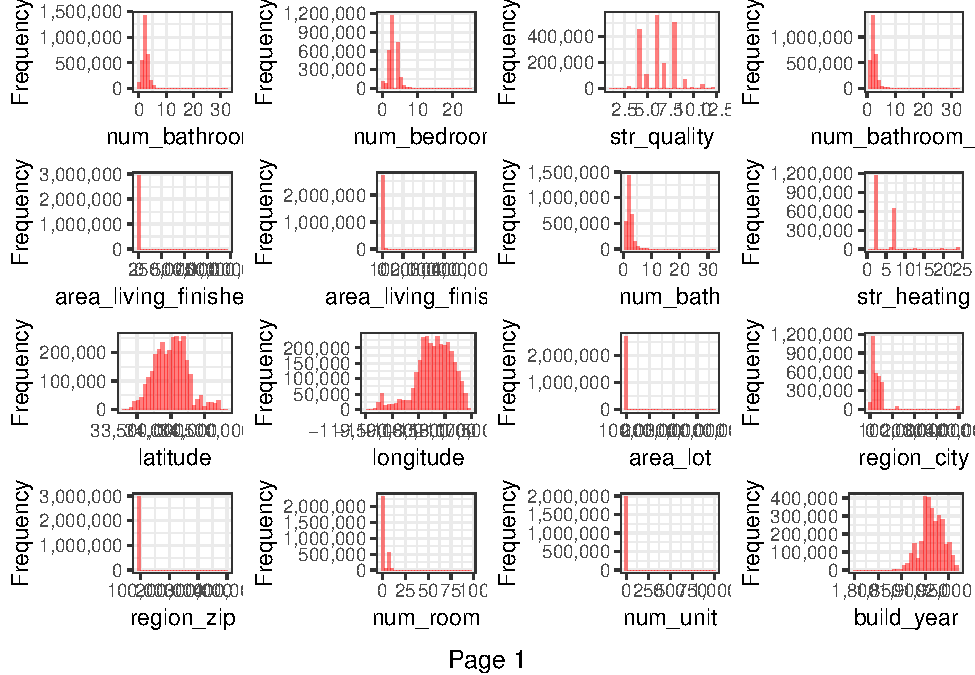
\includegraphics{zillow-prize_files/figure-latex/num-hist-1.pdf}
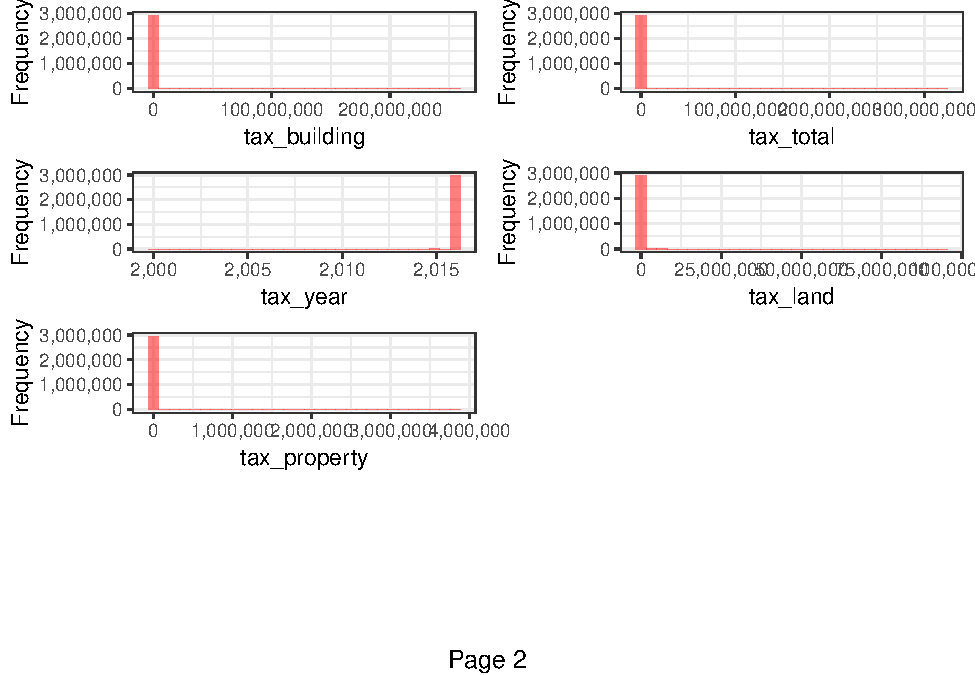
\includegraphics{zillow-prize_files/figure-latex/num-hist-2.pdf}

Looking at the histograms a few things become obvious. There are huge
outliers in many of the features and there are some features that are
currently encoded as numeric but should not be treated as such. For
example, \texttt{str\_quality} is an ordinal scale 1 (best qaulity) to
12 (worst) but if we leave them as numeric they will be treated as
ratio. \texttt{str\_heating} is nominal so the order doesn't have
meaning. Other that need to be changed are \texttt{region\_city},
\texttt{region\_zip}

Once we do this, we'll look again at the relationships between our
numeric features.

\begin{Shaded}
\begin{Highlighting}[]
\NormalTok{properties <-}\StringTok{ }\NormalTok{properties }\OperatorTok
\StringTok{  }\KeywordTok{mutate}\NormalTok{(}
    \DataTypeTok{str_quality =} \KeywordTok{factor}\NormalTok{(str_quality, }
                         \DataTypeTok{levels =} \KeywordTok{min}\NormalTok{(str_quality, }\DataTypeTok{na.rm =} \OtherTok{TRUE}\NormalTok{)}\OperatorTok{:}\KeywordTok{max}\NormalTok{(str_quality, }\DataTypeTok{na.rm =} \OtherTok{TRUE}\NormalTok{), }
                         \DataTypeTok{ordered =} \OtherTok{TRUE}\NormalTok{),}
    \DataTypeTok{str_heating =} \KeywordTok{factor}\NormalTok{(str_heating,}
                         \DataTypeTok{levels =} \KeywordTok{na.omit}\NormalTok{(}\KeywordTok{unique}\NormalTok{(str_heating)),}
                         \DataTypeTok{ordered =} \OtherTok{FALSE}\NormalTok{),}
    \DataTypeTok{region_city =} \KeywordTok{factor}\NormalTok{(region_city,}
                         \DataTypeTok{levels =} \KeywordTok{na.omit}\NormalTok{(}\KeywordTok{unique}\NormalTok{(region_city)),}
                         \DataTypeTok{ordered =} \OtherTok{FALSE}\NormalTok{),}
    \DataTypeTok{region_zip =} \KeywordTok{factor}\NormalTok{(region_zip,}
                         \DataTypeTok{levels =} \KeywordTok{na.omit}\NormalTok{(}\KeywordTok{unique}\NormalTok{(region_zip)),}
                         \DataTypeTok{ordered =} \OtherTok{FALSE}\NormalTok{)}
\NormalTok{  )}
\end{Highlighting}
\end{Shaded}

\subsection{Numeric Outliers}\label{numeric-outliers}

Based on the histograms there looks to be lots of outliers in many of
our numeric features. Two groups of features pop out, the
\texttt{num\_*} features and the \texttt{tax\_*}features. Let's take a
closer look.

\begin{Shaded}
\begin{Highlighting}[]
\NormalTok{properties }\OperatorTok
\StringTok{  }\KeywordTok{select}\NormalTok{(}\KeywordTok{starts_with}\NormalTok{(}\StringTok{"num_"}\NormalTok{)) }\OperatorTok
\KeywordTok{plot_histogram}\NormalTok{(}\DataTypeTok{ggtheme =} \KeywordTok{theme_bw}\NormalTok{(),  }\DataTypeTok{fill =} \StringTok{"red"}\NormalTok{, }\DataTypeTok{alpha =} \FloatTok{0.5}\NormalTok{)}
\end{Highlighting}
\end{Shaded}

\begin{figure}
\centering
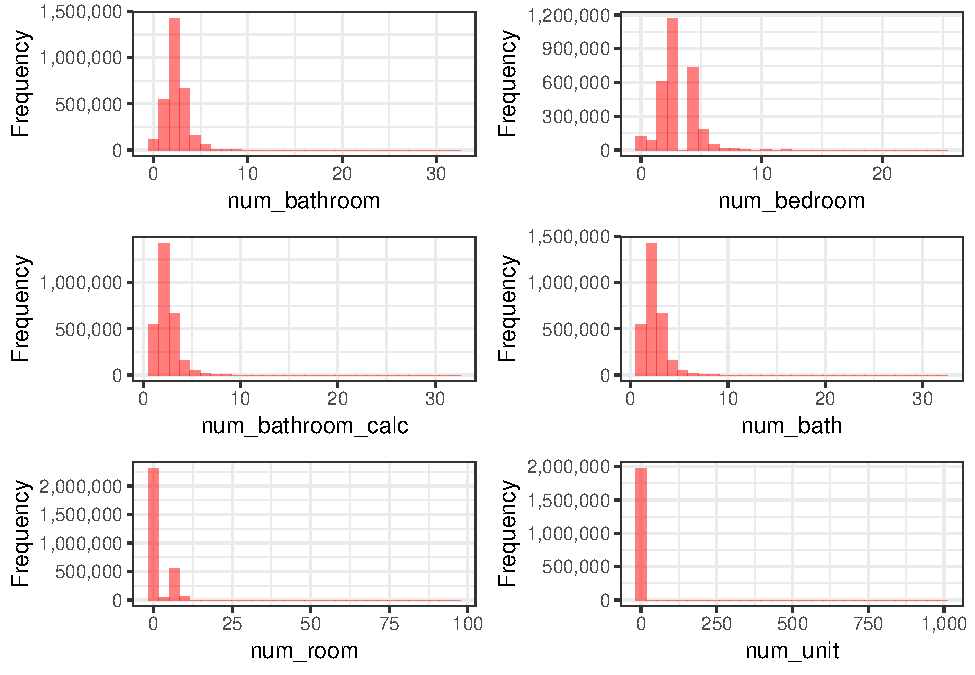
\includegraphics{zillow-prize_files/figure-latex/num-outlier-1.pdf}
\caption{\label{fig:num-outlier}Distriubtions of 'num\_*' Features}
\end{figure}

Looking at the \texttt{num\_bathroom}, \texttt{num\_bathroom\_calc},
\texttt{num\_bath} is pretty interesting. \texttt{num\_bathroom} was one
of the most complete features we had however, looking at the
distributions, it seems strange that there would be so many houses with
\texttt{0} bathrooms.

\begin{Shaded}
\begin{Highlighting}[]
\KeywordTok{sum}\NormalTok{(properties}\OperatorTok{$}\NormalTok{num_bathroom }\OperatorTok{==}\StringTok{ }\DecValTok{0}\NormalTok{, }\DataTypeTok{na.rm =} \OtherTok{TRUE}\NormalTok{)}
\end{Highlighting}
\end{Shaded}

\begin{verbatim}
## [1] 113470
\end{verbatim}

\begin{Shaded}
\begin{Highlighting}[]
\KeywordTok{sum}\NormalTok{(properties}\OperatorTok{$}\NormalTok{num_bathroom_calc }\OperatorTok{==}\StringTok{ }\DecValTok{0}\NormalTok{, }\DataTypeTok{na.rm =} \OtherTok{TRUE}\NormalTok{)}
\end{Highlighting}
\end{Shaded}

\begin{verbatim}
## [1] 0
\end{verbatim}

Now for comparing all 3

\begin{Shaded}
\begin{Highlighting}[]
\NormalTok{properties }\OperatorTok\StringTok{ }
\StringTok{  }\KeywordTok{group_by}\NormalTok{(}
\NormalTok{    num_bathroom_calc, }
\NormalTok{    num_bath, }
\NormalTok{    num_bathroom}
\NormalTok{    ) }\OperatorTok\StringTok{ }
\StringTok{  }\KeywordTok{count}\NormalTok{() }\OperatorTok
\StringTok{  }\NormalTok{DT}\OperatorTok{::}\KeywordTok{datatable}\NormalTok{()}
\end{Highlighting}
\end{Shaded}

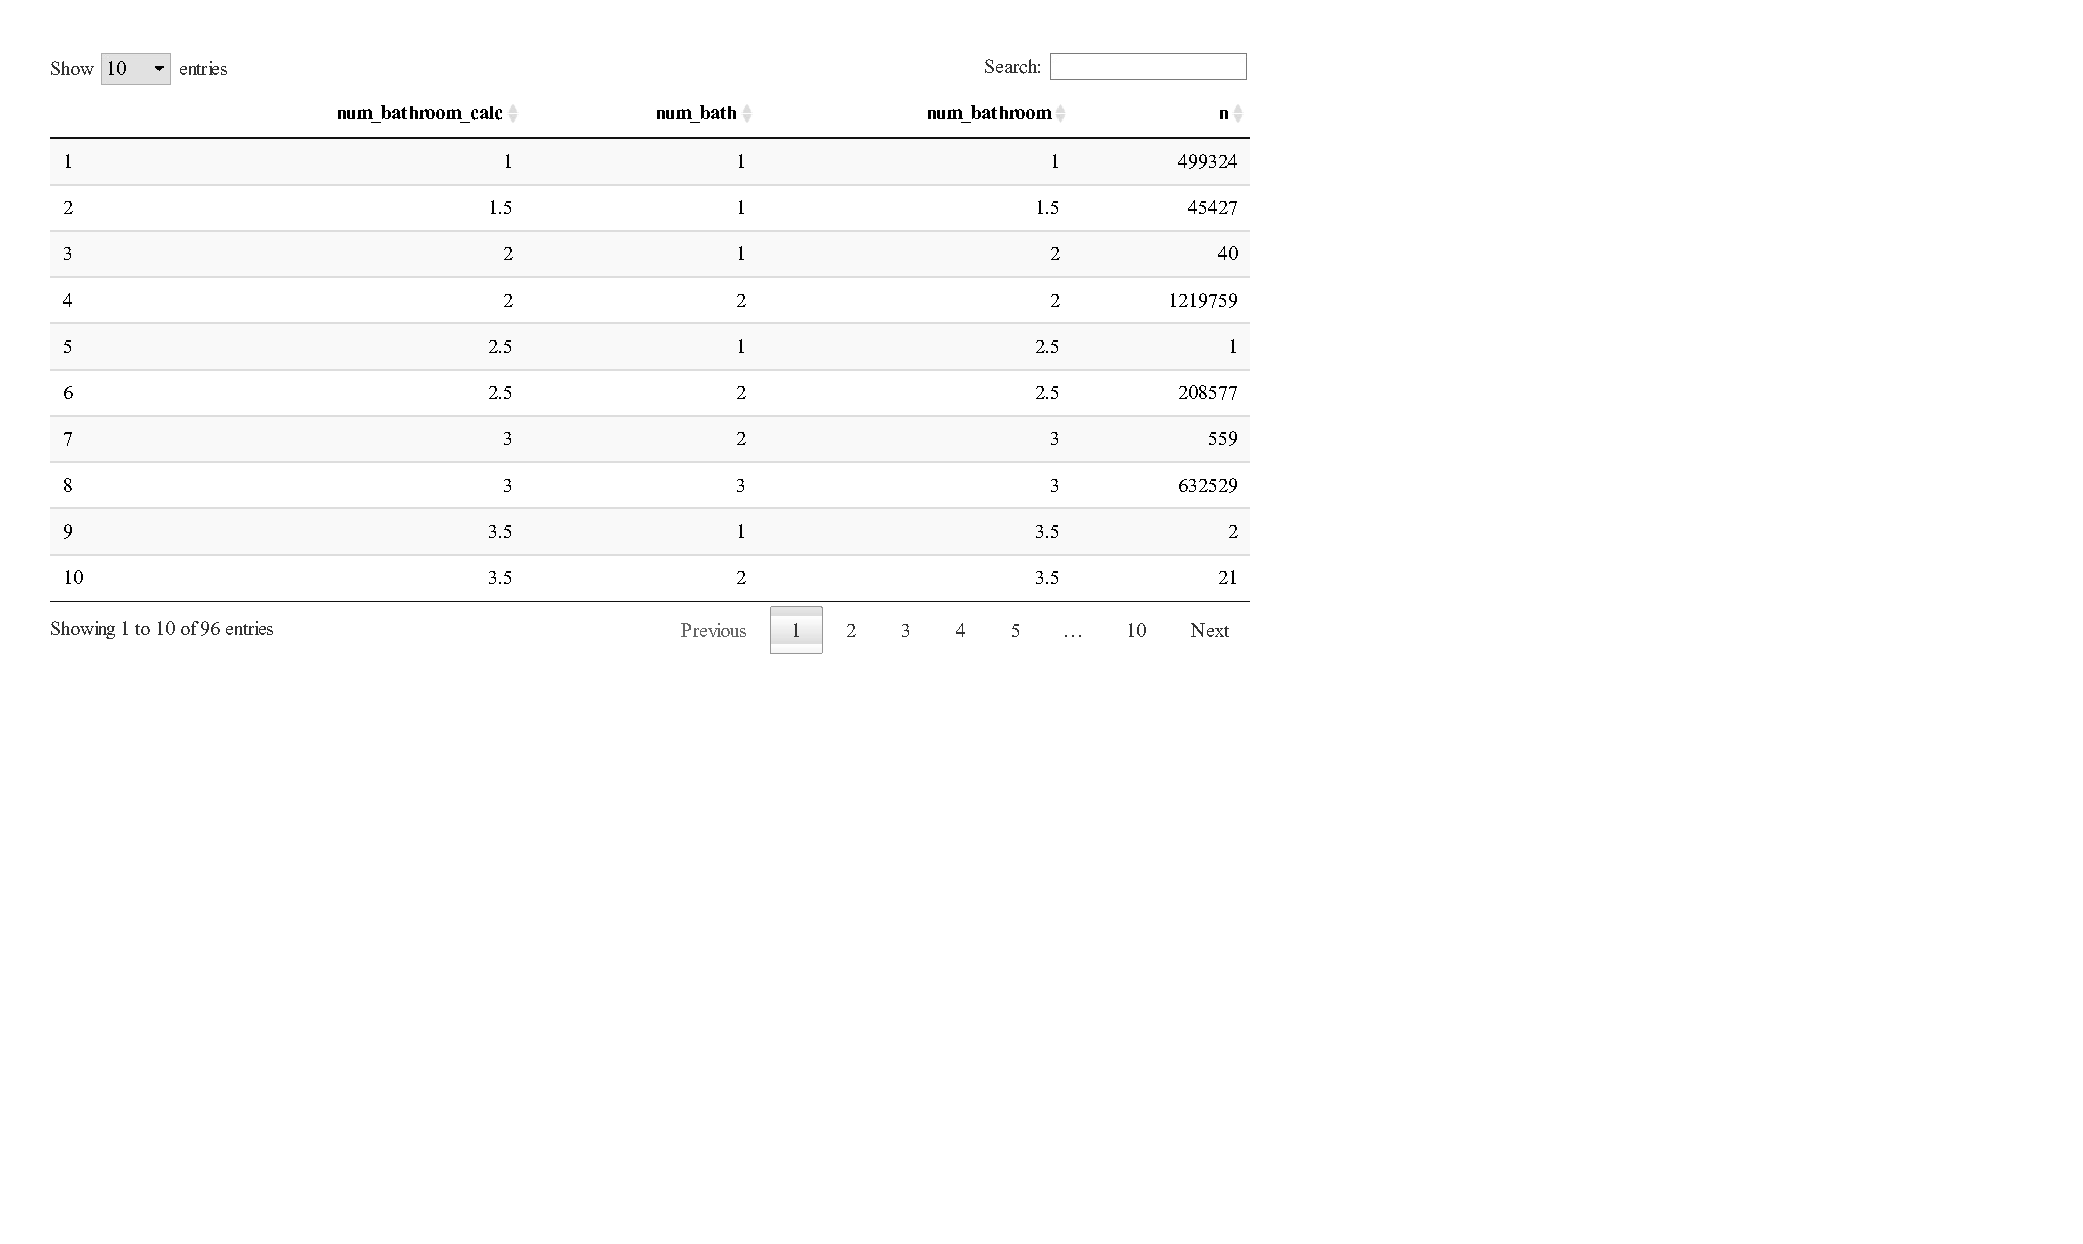
\includegraphics{zillow-prize_files/figure-latex/bath-compare-1.pdf}

If you sort by descending by \texttt{n} you'll see that one of the most
frequent combinations is blank values of \texttt{num\_bathroom\_calc}
and \texttt{num\_bath} which are \texttt{NA} values and \texttt{0} for
\texttt{num\_bathroom}. Based on this I am interpreting that as either
\texttt{0} being a coded value for \texttt{NA} or it just being wrong.
Either way it looks like \texttt{num\_bathroom\_calc} is the one to keep
out of all 3, since it has calculations of half-baths as well.

Applying the same logic to \texttt{num\_room} and \texttt{num\_bedroom}
we can set all values equal to \texttt{0} to \texttt{NA}. One side
effect of this is that the \texttt{num\_room} feature is now almost
100\% missing and not very useful anymore. So we will just remove it.

Quickly looking at \texttt{area\_living\_finished\_calc} and
\texttt{area\_living\_finished} reveals a similar \texttt{*\_calc} being
a corrected version of the feature. Becasue of this we will go ahead and
remove \texttt{area\_living\_finished} as well

\begin{Shaded}
\begin{Highlighting}[]
\NormalTok{properties <-}\StringTok{ }\NormalTok{properties }\OperatorTok
\StringTok{  }\KeywordTok{select}\NormalTok{(}
    \OperatorTok{-}\NormalTok{num_bath,}
    \OperatorTok{-}\NormalTok{num_bathroom,}
    \OperatorTok{-}\NormalTok{num_room,}
    \OperatorTok{-}\NormalTok{area_living_finished}
\NormalTok{    ) }\OperatorTok
\StringTok{  }\KeywordTok{mutate}\NormalTok{(}
    \DataTypeTok{num_bedroom =} \KeywordTok{ifelse}\NormalTok{(num_bedroom }\OperatorTok{==}\StringTok{ }\DecValTok{0}\NormalTok{, }\OtherTok{NA}\NormalTok{, num_bedroom)}
\NormalTok{    )}
\end{Highlighting}
\end{Shaded}

Now let's look at the tax related features

\begin{Shaded}
\begin{Highlighting}[]
\NormalTok{properties }\OperatorTok
\StringTok{  }\KeywordTok{select}\NormalTok{(}\KeywordTok{starts_with}\NormalTok{(}\StringTok{"tax_"}\NormalTok{)) }\OperatorTok
\KeywordTok{plot_histogram}\NormalTok{(}\DataTypeTok{ggtheme =} \KeywordTok{theme_bw}\NormalTok{(),  }\DataTypeTok{fill =} \StringTok{"red"}\NormalTok{, }\DataTypeTok{alpha =} \FloatTok{0.5}\NormalTok{)}
\end{Highlighting}
\end{Shaded}

\begin{figure}
\centering
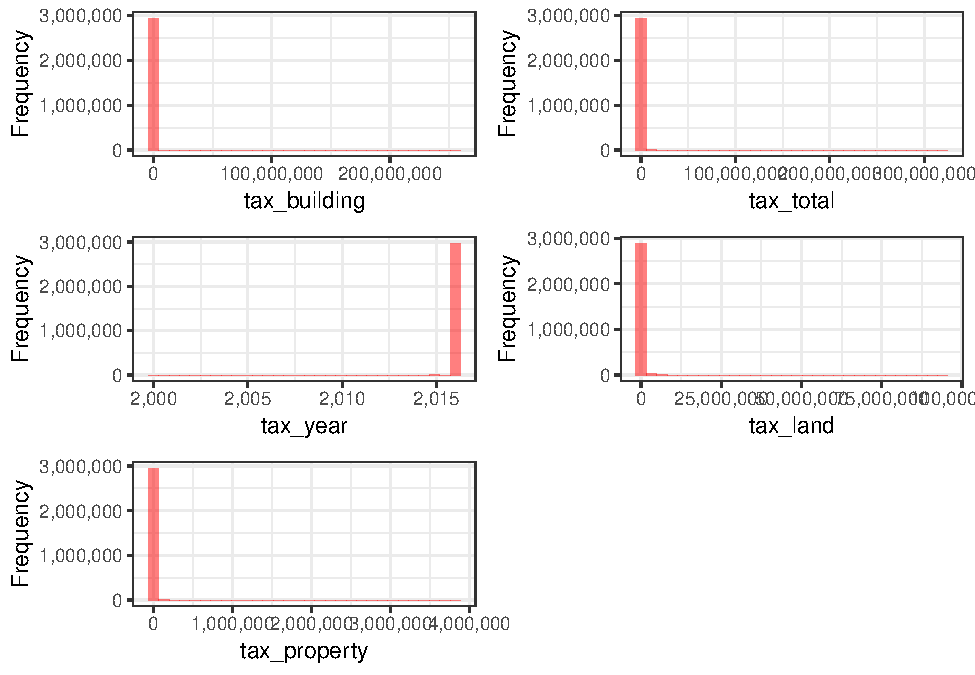
\includegraphics{zillow-prize_files/figure-latex/tax-outlier-1.pdf}
\caption{\label{fig:tax-outlier}Distriubtions of 'tax\_*' Features}
\end{figure}

Lets look at the highest values for \texttt{tax\_total} and see if
something jumps out

\begin{Shaded}
\begin{Highlighting}[]
\NormalTok{properties }\OperatorTok\StringTok{ }
\StringTok{  }\KeywordTok{mutate}\NormalTok{(}\DataTypeTok{tax_rank =} \KeywordTok{rank}\NormalTok{(}\KeywordTok{desc}\NormalTok{(tax_total))) }\OperatorTok\StringTok{ }
\StringTok{  }\KeywordTok{filter}\NormalTok{(tax_rank }\OperatorTok{<=}\StringTok{ }\DecValTok{20}\NormalTok{) }\OperatorTok\StringTok{ }
\StringTok{  }\KeywordTok{select}\NormalTok{(}
\NormalTok{    zoning_landuse, }
    \KeywordTok{starts_with}\NormalTok{(}\StringTok{"area_"}\NormalTok{), }
    \KeywordTok{starts_with}\NormalTok{(}\StringTok{"tax_"}\NormalTok{)}
\NormalTok{    ) }\OperatorTok\StringTok{ }
\StringTok{  }\KeywordTok{arrange}\NormalTok{(tax_rank) }\OperatorTok
\StringTok{  }\NormalTok{DT}\OperatorTok{::}\KeywordTok{datatable}\NormalTok{(}
    \DataTypeTok{extensions =} \StringTok{'FixedColumns'}\NormalTok{,}
    \DataTypeTok{options =} \KeywordTok{list}\NormalTok{(}
    \DataTypeTok{dom =} \StringTok{'t'}\NormalTok{,}
    \DataTypeTok{scrollX =} \OtherTok{TRUE}\NormalTok{,}
    \DataTypeTok{scrollCollapse =} \OtherTok{TRUE}
\NormalTok{    )}
\NormalTok{    )}
\end{Highlighting}
\end{Shaded}

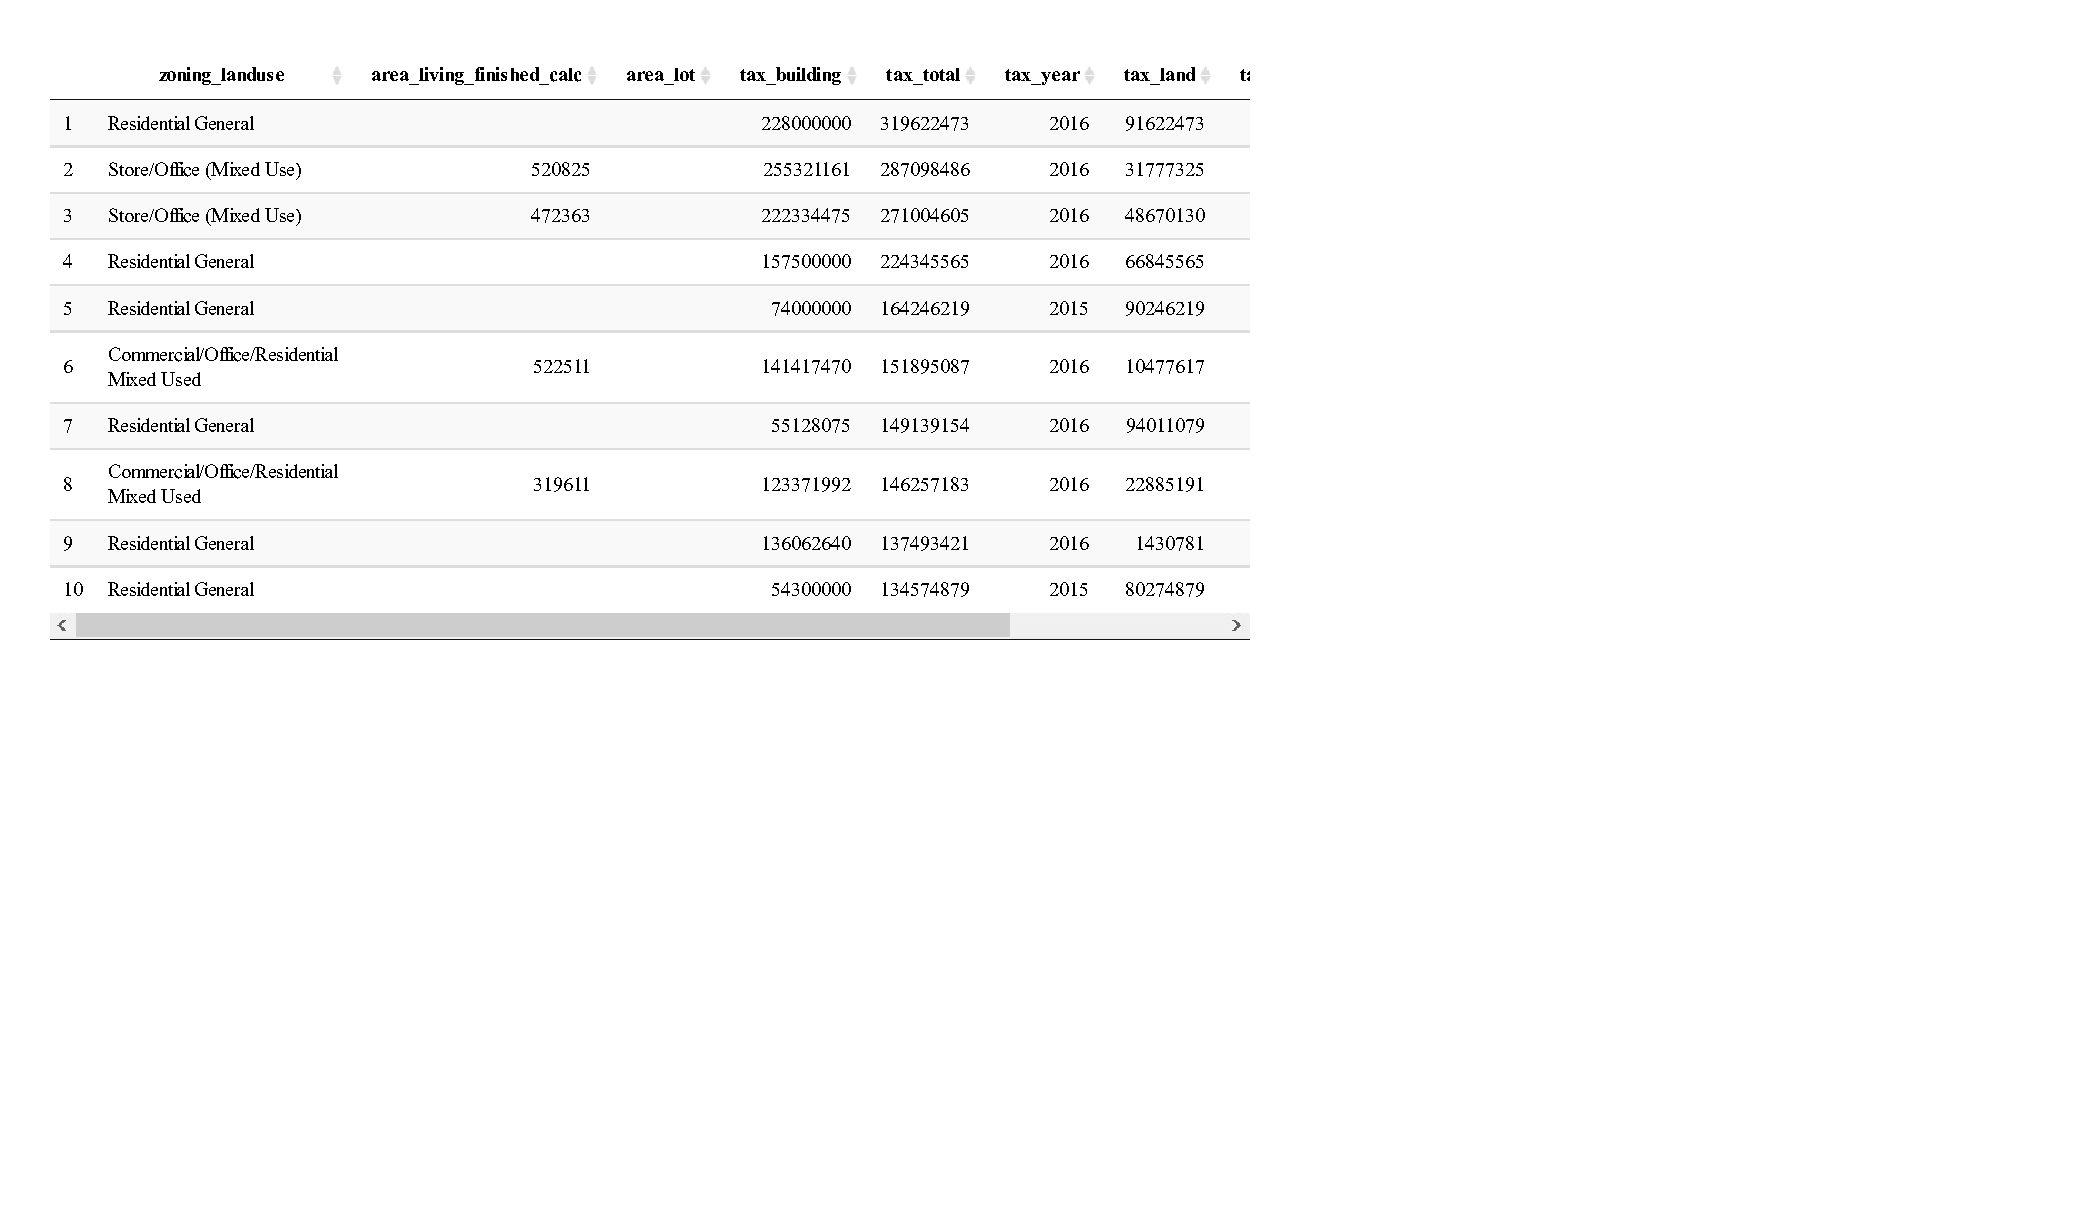
\includegraphics{zillow-prize_files/figure-latex/unnamed-chunk-4-1.pdf}

While the values are extremely large, they appear to look legitimate. We
won't remove these, but it does indicate that we should perhaps apply
some transformations to our tax features before we start applying our
model.

Now a look at the relationships between our remaining numeric features

\begin{Shaded}
\begin{Highlighting}[]
\KeywordTok{library}\NormalTok{(heatmaply)}

\NormalTok{properties }\OperatorTok
\StringTok{  }\KeywordTok{select}\NormalTok{(}\OperatorTok{-}\NormalTok{id_parcel) }\OperatorTok
\StringTok{  }\KeywordTok{select_if}\NormalTok{(is.numeric) }\OperatorTok
\StringTok{  }\KeywordTok{cor}\NormalTok{(}\DataTypeTok{use =} \StringTok{"pairwise.complete.obs"}\NormalTok{) }\OperatorTok
\StringTok{  }\KeywordTok{heatmaply_cor}\NormalTok{()}
\end{Highlighting}
\end{Shaded}

\begin{figure}
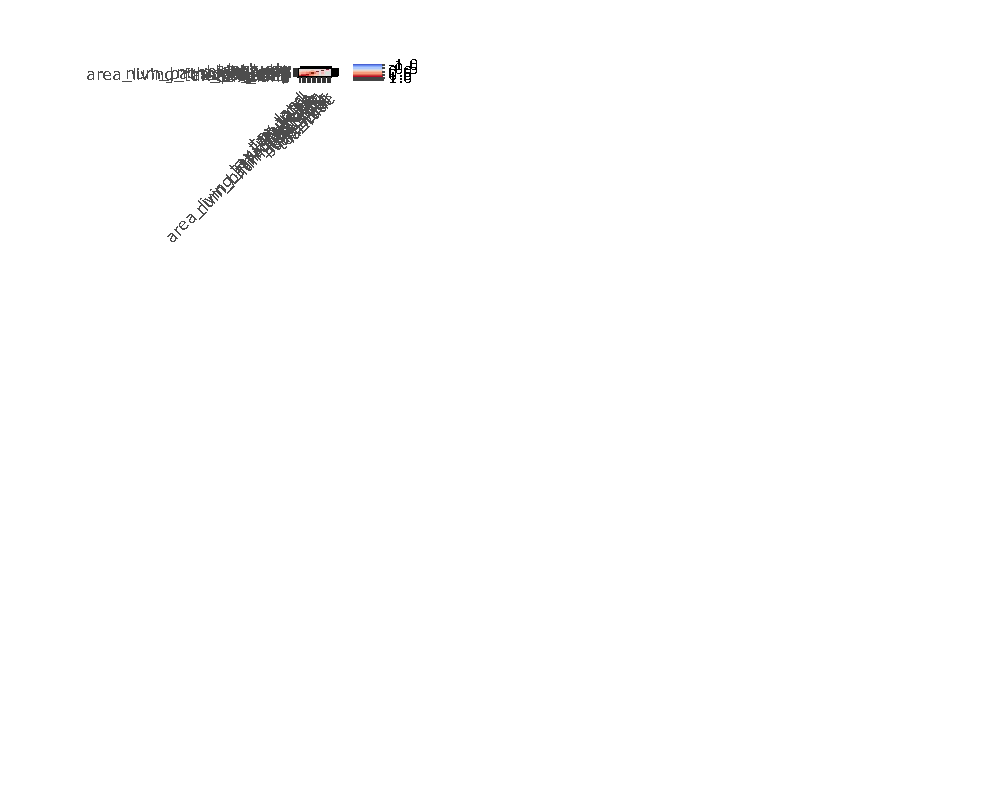
\includegraphics[width=1\linewidth]{zillow-prize_files/figure-latex/num-cor-heatmap-1} \caption{Correlation of Numeric Features}\label{fig:num-cor-heatmap}
\end{figure}

\subsection{Categorical Features}\label{categorical-features}

\begin{Shaded}
\begin{Highlighting}[]
\KeywordTok{plot_bar}\NormalTok{(properties, }\DataTypeTok{ggtheme =} \KeywordTok{theme_bw}\NormalTok{())}
\end{Highlighting}
\end{Shaded}

\begin{verbatim}
## 2 columns ignored with more than 50 categories.
## region_city: 187 categories
## region_zip: 404 categories
\end{verbatim}

\begin{figure}
\centering
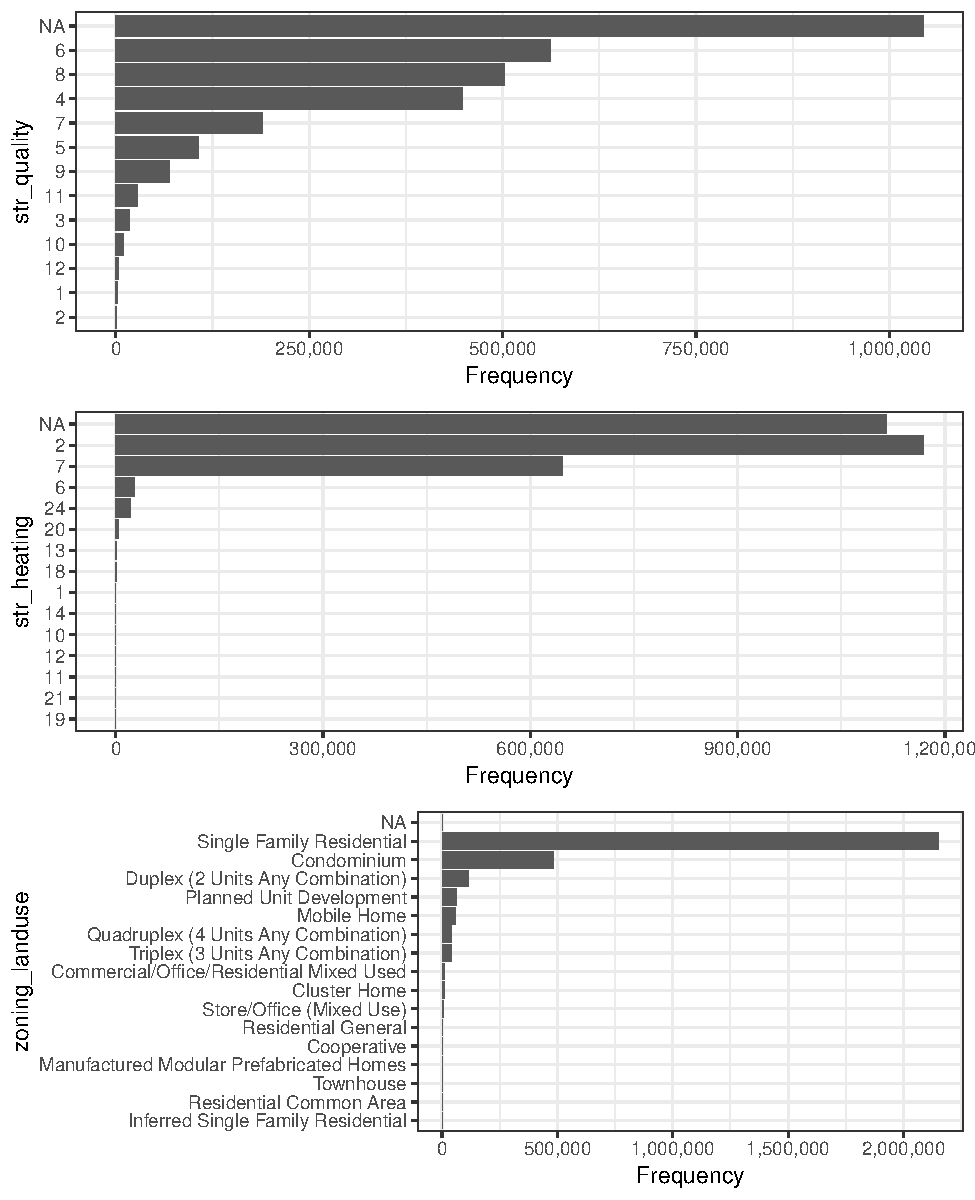
\includegraphics{zillow-prize_files/figure-latex/prop-bars-1.pdf}
\caption{\label{fig:prop-bars}Distriubtions of All Categorical Features}
\end{figure}

The distribution across categories are extremely non-uniform, especially
\texttt{str\_heating} and \texttt{zoning\_landuse}. This imbalance could
cause use some pain later one when trying to fit our model. One way we
can avoid some of this pain is by collapsing some of the rare categories
into an \texttt{other} category. The number of categories we collapse to
is not a hard and fast decision, it can be based on number of
observations, subject matter expertise, heterogentity of the response
variable within categories, or some mix of all of these).

Let's look at what the distribution of \texttt{log\_error} looks like
across these categories.

\begin{Shaded}
\begin{Highlighting}[]
\KeywordTok{library}\NormalTok{(ggridges)}

\NormalTok{properties }\OperatorTok
\StringTok{  }\KeywordTok{select}\NormalTok{(}
\NormalTok{    id_parcel,}
\NormalTok{    str_quality}
\NormalTok{  ) }\OperatorTok
\StringTok{  }\KeywordTok{right_join}\NormalTok{(trans, }\DataTypeTok{by =} \StringTok{"id_parcel"}\NormalTok{) }\OperatorTok
\StringTok{  }\KeywordTok{ggplot}\NormalTok{(}\KeywordTok{aes}\NormalTok{(}\DataTypeTok{x =}\NormalTok{ log_error, }\DataTypeTok{y =} \KeywordTok{fct_reorder}\NormalTok{(str_quality, log_error), }\DataTypeTok{fill =} \KeywordTok{factor}\NormalTok{(..quantile..))) }\OperatorTok{+}\StringTok{  }
\StringTok{  }\KeywordTok{stat_density_ridges}\NormalTok{(}
    \DataTypeTok{geom =} \StringTok{"density_ridges_gradient"}\NormalTok{, }
    \DataTypeTok{calc_ecdf =} \OtherTok{TRUE}\NormalTok{, }
    \DataTypeTok{quantiles =} \KeywordTok{c}\NormalTok{(}\FloatTok{0.05}\NormalTok{, }\FloatTok{0.95}\NormalTok{)}
\NormalTok{    ) }\OperatorTok{+}
\StringTok{  }\KeywordTok{scale_fill_manual}\NormalTok{(}
    \DataTypeTok{name =} \StringTok{"Probability"}\NormalTok{, }
    \DataTypeTok{values =} \KeywordTok{c}\NormalTok{(}\StringTok{"#FF0000A0"}\NormalTok{, }\StringTok{"#A0A0A0A0"}\NormalTok{, }\StringTok{"#0000FFA0"}\NormalTok{),}
    \DataTypeTok{labels =} \KeywordTok{c}\NormalTok{(}\StringTok{"(0, 0.05]"}\NormalTok{, }\StringTok{"(0.05, 0.95]"}\NormalTok{, }\StringTok{"(0.95, 1]"}\NormalTok{)}
\NormalTok{    ) }\OperatorTok{+}
\StringTok{  }\KeywordTok{xlim}\NormalTok{(}\KeywordTok{c}\NormalTok{(}\OperatorTok{-}\FloatTok{0.5}\NormalTok{, }\FloatTok{0.5}\NormalTok{)) }\OperatorTok{+}
\StringTok{  }\KeywordTok{theme_bw}\NormalTok{() }\OperatorTok{+}
\StringTok{  }\KeywordTok{labs}\NormalTok{(}
    \DataTypeTok{y =} \StringTok{"str_quality"}
\NormalTok{  )}
\end{Highlighting}
\end{Shaded}

\begin{figure}
\centering
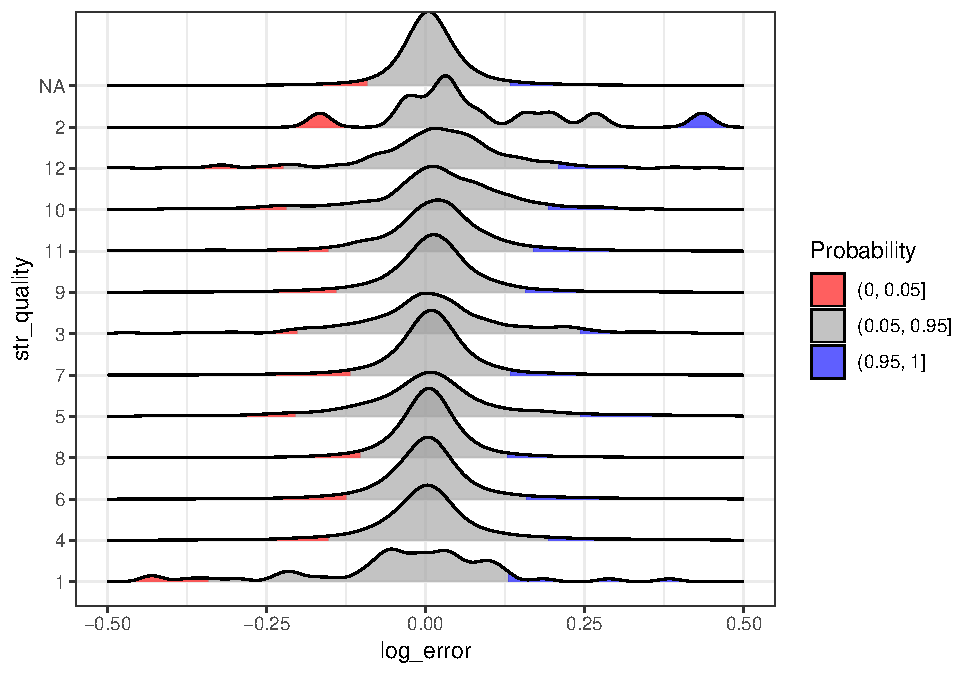
\includegraphics{zillow-prize_files/figure-latex/le-by-str-qaul-1.pdf}
\caption{\label{fig:le-by-str-qaul}Distribution of Log Error Across
Structure Quality Feature}
\end{figure}

\begin{Shaded}
\begin{Highlighting}[]
\KeywordTok{library}\NormalTok{(ggridges)}

\NormalTok{properties }\OperatorTok
\StringTok{  }\KeywordTok{select}\NormalTok{(}
\NormalTok{    id_parcel,}
\NormalTok{    str_heating}
\NormalTok{  ) }\OperatorTok
\StringTok{  }\KeywordTok{right_join}\NormalTok{(trans, }\DataTypeTok{by =} \StringTok{"id_parcel"}\NormalTok{) }\OperatorTok
\StringTok{  }\KeywordTok{ggplot}\NormalTok{(}\KeywordTok{aes}\NormalTok{(}\DataTypeTok{x =}\NormalTok{ log_error, }\DataTypeTok{y =} \KeywordTok{fct_reorder}\NormalTok{(str_heating, log_error), }\DataTypeTok{fill =} \KeywordTok{factor}\NormalTok{(..quantile..))) }\OperatorTok{+}\StringTok{  }
\StringTok{  }\KeywordTok{stat_density_ridges}\NormalTok{(}
    \DataTypeTok{geom =} \StringTok{"density_ridges_gradient"}\NormalTok{, }
    \DataTypeTok{calc_ecdf =} \OtherTok{TRUE}\NormalTok{, }
    \DataTypeTok{quantiles =} \KeywordTok{c}\NormalTok{(}\FloatTok{0.05}\NormalTok{, }\FloatTok{0.95}\NormalTok{)}
\NormalTok{    ) }\OperatorTok{+}
\StringTok{  }\KeywordTok{scale_fill_manual}\NormalTok{(}
    \DataTypeTok{name =} \StringTok{"Probability"}\NormalTok{, }
    \DataTypeTok{values =} \KeywordTok{c}\NormalTok{(}\StringTok{"#FF0000A0"}\NormalTok{, }\StringTok{"#A0A0A0A0"}\NormalTok{, }\StringTok{"#0000FFA0"}\NormalTok{),}
    \DataTypeTok{labels =} \KeywordTok{c}\NormalTok{(}\StringTok{"(0, 0.05]"}\NormalTok{, }\StringTok{"(0.05, 0.95]"}\NormalTok{, }\StringTok{"(0.95, 1]"}\NormalTok{)}
\NormalTok{    ) }\OperatorTok{+}
\StringTok{  }\KeywordTok{xlim}\NormalTok{(}\KeywordTok{c}\NormalTok{(}\OperatorTok{-}\FloatTok{0.5}\NormalTok{, }\FloatTok{0.5}\NormalTok{)) }\OperatorTok{+}
\StringTok{  }\KeywordTok{theme_bw}\NormalTok{() }\OperatorTok{+}
\StringTok{  }\KeywordTok{labs}\NormalTok{(}
    \DataTypeTok{y =} \StringTok{"str_heating"}
\NormalTok{  )}
\end{Highlighting}
\end{Shaded}

\begin{figure}
\centering
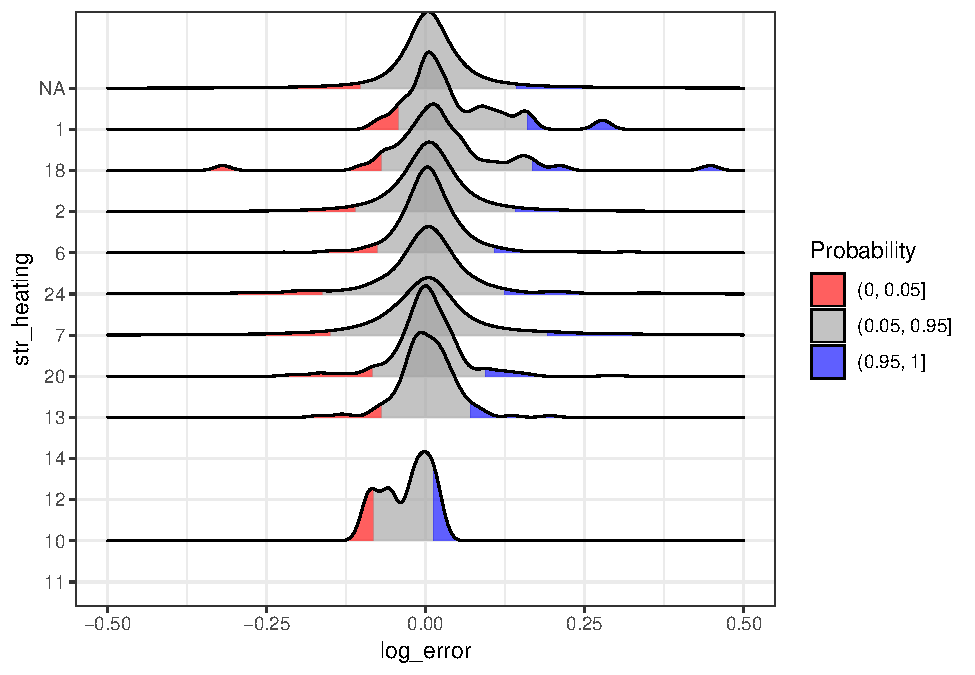
\includegraphics{zillow-prize_files/figure-latex/le-by-str-heating-1.pdf}
\caption{\label{fig:le-by-str-heating}Distribution of Log Error Across
Heating Type Feature}
\end{figure}

\begin{Shaded}
\begin{Highlighting}[]
\KeywordTok{library}\NormalTok{(ggridges)}

\NormalTok{properties }\OperatorTok
\StringTok{  }\KeywordTok{select}\NormalTok{(}
\NormalTok{    id_parcel,}
\NormalTok{    zoning_landuse}
\NormalTok{  ) }\OperatorTok
\StringTok{  }\KeywordTok{right_join}\NormalTok{(trans, }\DataTypeTok{by =} \StringTok{"id_parcel"}\NormalTok{) }\OperatorTok
\StringTok{  }\KeywordTok{ggplot}\NormalTok{(}\KeywordTok{aes}\NormalTok{(}\DataTypeTok{x =}\NormalTok{ log_error, }\DataTypeTok{y =} \KeywordTok{fct_reorder}\NormalTok{(zoning_landuse, log_error), }\DataTypeTok{fill =} \KeywordTok{factor}\NormalTok{(..quantile..))) }\OperatorTok{+}\StringTok{  }
\StringTok{  }\KeywordTok{stat_density_ridges}\NormalTok{(}
    \DataTypeTok{geom =} \StringTok{"density_ridges_gradient"}\NormalTok{, }
    \DataTypeTok{calc_ecdf =} \OtherTok{TRUE}\NormalTok{, }
    \DataTypeTok{quantiles =} \KeywordTok{c}\NormalTok{(}\FloatTok{0.05}\NormalTok{, }\FloatTok{0.95}\NormalTok{)}
\NormalTok{    ) }\OperatorTok{+}
\StringTok{  }\KeywordTok{scale_fill_manual}\NormalTok{(}
    \DataTypeTok{name =} \StringTok{"Probability"}\NormalTok{, }
    \DataTypeTok{values =} \KeywordTok{c}\NormalTok{(}\StringTok{"#FF0000A0"}\NormalTok{, }\StringTok{"#A0A0A0A0"}\NormalTok{, }\StringTok{"#0000FFA0"}\NormalTok{),}
    \DataTypeTok{labels =} \KeywordTok{c}\NormalTok{(}\StringTok{"(0, 0.05]"}\NormalTok{, }\StringTok{"(0.05, 0.95]"}\NormalTok{, }\StringTok{"(0.95, 1]"}\NormalTok{)}
\NormalTok{    ) }\OperatorTok{+}
\StringTok{  }\KeywordTok{xlim}\NormalTok{(}\KeywordTok{c}\NormalTok{(}\OperatorTok{-}\FloatTok{0.5}\NormalTok{, }\FloatTok{0.5}\NormalTok{)) }\OperatorTok{+}
\StringTok{  }\KeywordTok{theme_bw}\NormalTok{() }\OperatorTok{+}
\StringTok{  }\KeywordTok{labs}\NormalTok{(}
    \DataTypeTok{y =} \StringTok{"zoning_landuse"}
\NormalTok{  )}
\end{Highlighting}
\end{Shaded}

\begin{figure}
\centering
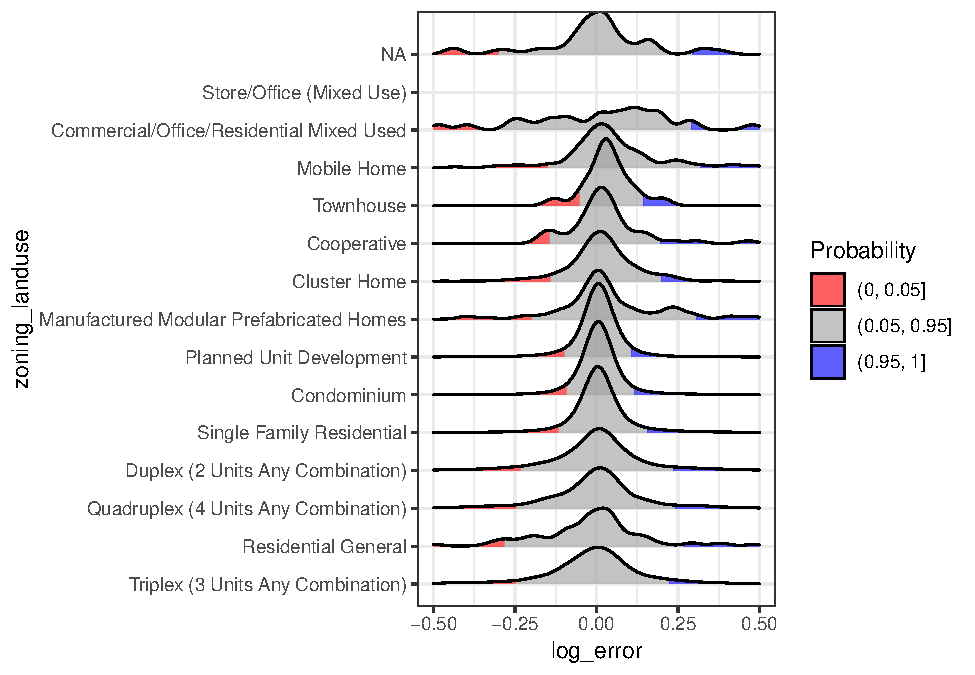
\includegraphics{zillow-prize_files/figure-latex/le-by-zoning-1.pdf}
\caption{\label{fig:le-by-zoning}Distribution of Log Error Across Zoning
Feature}
\end{figure}

Since the distributions of \texttt{log\_error} within each category
seems well behaved, we will recode them based on number of observations

\begin{Shaded}
\begin{Highlighting}[]
\NormalTok{properties <-}\StringTok{ }\NormalTok{properties }\OperatorTok
\StringTok{  }\KeywordTok{mutate}\NormalTok{(}
    \DataTypeTok{str_heating =} \KeywordTok{fct_lump}\NormalTok{(str_heating, }\DataTypeTok{n =} \DecValTok{6}\NormalTok{),}
    \DataTypeTok{zoning_landuse =} \KeywordTok{fct_lump}\NormalTok{(zoning_landuse, }\DataTypeTok{n =} \DecValTok{8}\NormalTok{),}
    \DataTypeTok{str_heating =} \KeywordTok{fct_recode}\NormalTok{(str_heating,}
      \StringTok{"Central"}\NormalTok{ =}\StringTok{ "2"}\NormalTok{,}
      \StringTok{"Floor/Wall"}\NormalTok{ =}\StringTok{ "7"}\NormalTok{,}
      \StringTok{"Solar"}\NormalTok{ =}\StringTok{ "20"}\NormalTok{,}
      \StringTok{"Forced Air"}\NormalTok{ =}\StringTok{ "6"}\NormalTok{,}
      \StringTok{"Yes - Type Unknown"}\NormalTok{ =}\StringTok{ "24"}\NormalTok{,}
      \StringTok{"None"}\NormalTok{ =}\StringTok{ "13"}
\NormalTok{    )}
\NormalTok{  )}
\end{Highlighting}
\end{Shaded}

\section{\texorpdfstring{Exploring \texttt{log\_error} A little
More}{Exploring log\_error A little More}}\label{exploring-log_error-a-little-more}

Now let's join the \texttt{properties} and \texttt{properties\_geo}
tables to our \texttt{trans} table of tranactions and their
\texttt{log\_error}'s and explore those

\begin{Shaded}
\begin{Highlighting}[]
\NormalTok{trans_prop <-}\StringTok{ }\KeywordTok{read_feather}\NormalTok{(}\StringTok{"data/properties_geo_only.feather"}\NormalTok{) }\OperatorTok
\StringTok{  }\KeywordTok{right_join}\NormalTok{(trans, }\DataTypeTok{by =} \StringTok{"id_parcel"}\NormalTok{) }\OperatorTok
\StringTok{  }\KeywordTok{left_join}\NormalTok{(properties, }\DataTypeTok{by =} \StringTok{"id_parcel"}\NormalTok{)}
\end{Highlighting}
\end{Shaded}

\begin{Shaded}
\begin{Highlighting}[]
\NormalTok{trans_prop }\OperatorTok
\StringTok{  }\KeywordTok{group_by}\NormalTok{(id_geo_bg_fips, id_geo_county_name) }\OperatorTok
\StringTok{  }\KeywordTok{summarise}\NormalTok{(}
    \DataTypeTok{n =} \KeywordTok{n}\NormalTok{(),}
    \DataTypeTok{mean_abs_error =} \KeywordTok{mean}\NormalTok{(abs_log_error)}
\NormalTok{    ) }\OperatorTok
\StringTok{  }\KeywordTok{ungroup}\NormalTok{() }\OperatorTok
\StringTok{  }\KeywordTok{mutate}\NormalTok{(}
    \DataTypeTok{trans_pert =} \KeywordTok{cut}\NormalTok{(n, }\DataTypeTok{breaks =} \KeywordTok{c}\NormalTok{(}\KeywordTok{seq}\NormalTok{(}\DecValTok{0}\NormalTok{, }\DecValTok{100}\NormalTok{, }\DecValTok{10}\NormalTok{), }\DecValTok{350}\NormalTok{))}
\NormalTok{    ) }\OperatorTok
\StringTok{  }\KeywordTok{ggplot}\NormalTok{(}\KeywordTok{aes}\NormalTok{(}\DataTypeTok{x =}\NormalTok{ trans_pert, }\DataTypeTok{y =}\NormalTok{ mean_abs_error, }\DataTypeTok{colour =}\NormalTok{ id_geo_county_name)) }\OperatorTok{+}\StringTok{ }
\StringTok{  }\KeywordTok{geom_boxplot}\NormalTok{(}\DataTypeTok{outlier.size =} \FloatTok{1.5}\NormalTok{, }\DataTypeTok{outlier.alpha =} \DecValTok{1}\OperatorTok{/}\DecValTok{3}\NormalTok{) }\OperatorTok{+}
\StringTok{  }\KeywordTok{theme_bw}\NormalTok{() }\OperatorTok{+}
\StringTok{  }\KeywordTok{labs}\NormalTok{(}
    \DataTypeTok{subtitle =} \StringTok{"Block Group Average Mean Absolute Error"}\NormalTok{,}
    \DataTypeTok{colour =} \OtherTok{NULL}\NormalTok{,}
    \DataTypeTok{x =} \StringTok{"Number of Total Transactions per Block Group"}\NormalTok{,}
    \DataTypeTok{y =} \StringTok{"Mean Absolute Log Error"}
\NormalTok{  )}
\end{Highlighting}
\end{Shaded}

\begin{figure}
\centering
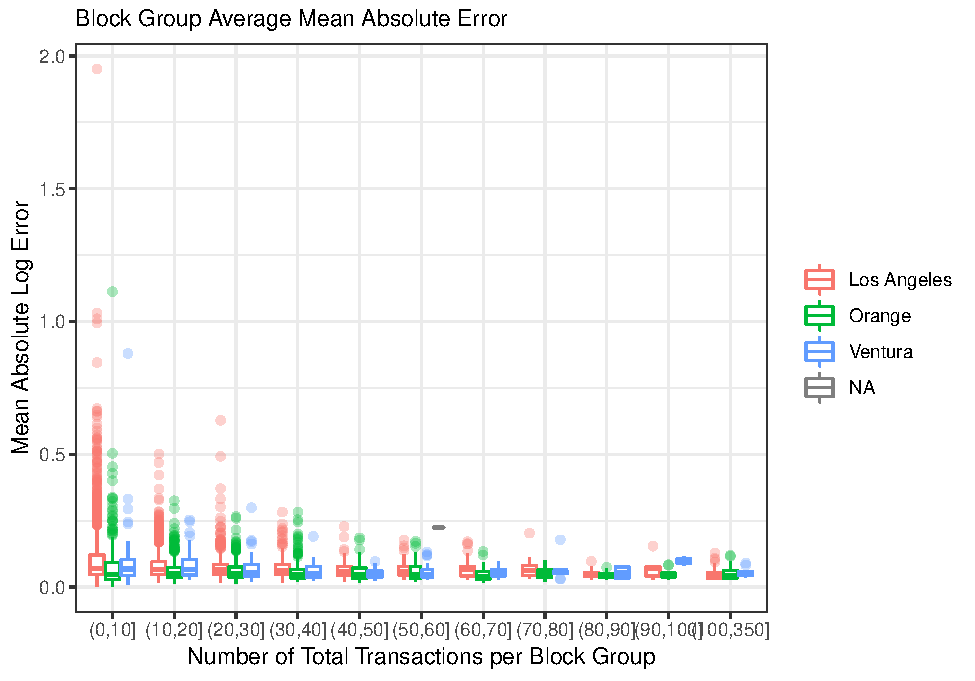
\includegraphics{zillow-prize_files/figure-latex/le-bg-box-1.pdf}
\caption{\label{fig:le-bg-box}Outliers and Variability of Mean Absolute
Error Dreceases When Neighborhood Sales Increase}
\end{figure}

It looks like Los Angeles is largerly the only county that has
information populated for \texttt{str\_qaulity}

\begin{Shaded}
\begin{Highlighting}[]
\NormalTok{trans_prop }\OperatorTok
\StringTok{  }\KeywordTok{ggplot}\NormalTok{(}\KeywordTok{aes}\NormalTok{(}\DataTypeTok{x =}\NormalTok{ str_quality, }\DataTypeTok{y =}\NormalTok{ log_error, }\DataTypeTok{colour =}\NormalTok{ id_geo_county_name)) }\OperatorTok{+}\StringTok{ }
\StringTok{  }\KeywordTok{geom_boxplot}\NormalTok{(}\DataTypeTok{outlier.size =} \FloatTok{1.5}\NormalTok{, }\DataTypeTok{outlier.alpha =} \DecValTok{1}\OperatorTok{/}\DecValTok{3}\NormalTok{) }\OperatorTok{+}
\StringTok{  }\KeywordTok{theme_bw}\NormalTok{() }\OperatorTok{+}
\StringTok{  }\KeywordTok{labs}\NormalTok{(}
    \DataTypeTok{colour =} \OtherTok{NULL}
\NormalTok{  )}
\end{Highlighting}
\end{Shaded}

\begin{figure}
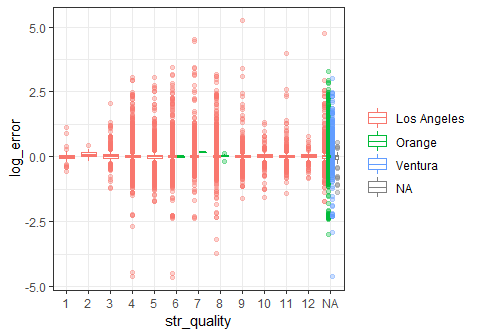
\includegraphics[width=1\linewidth]{zillow-prize_files/figure-latex/le-zone-box-1} \caption{Log Error by Structure Quality}\label{fig:le-zone-box}
\end{figure}

\begin{Shaded}
\begin{Highlighting}[]
\KeywordTok{library}\NormalTok{(ggmap)}

\NormalTok{trans_prop_tmp <-}\StringTok{ }\NormalTok{trans_prop }\OperatorTok
\StringTok{  }\KeywordTok{filter}\NormalTok{(}\OperatorTok{!}\KeywordTok{is.na}\NormalTok{(id_geo_county_name)) }\OperatorTok
\StringTok{  }\KeywordTok{group_by}\NormalTok{(}
\NormalTok{    id_parcel, }
\NormalTok{    id_geo_county_name}
\NormalTok{    ) }\OperatorTok
\StringTok{  }\KeywordTok{mutate}\NormalTok{(}
    \DataTypeTok{log_error_parcel_avg =} \KeywordTok{mean}\NormalTok{(log_error)}
\NormalTok{    ) }\OperatorTok
\StringTok{  }\KeywordTok{ungroup}\NormalTok{() }\OperatorTok
\StringTok{  }\KeywordTok{mutate}\NormalTok{(}
    \DataTypeTok{outlier =} \KeywordTok{ifelse}\NormalTok{(log_error }\OperatorTok{<}\StringTok{ }\KeywordTok{quantile}\NormalTok{(log_error, }\DataTypeTok{probs  =}\NormalTok{ .}\DecValTok{1}\NormalTok{) }\OperatorTok{|}\StringTok{ }
\StringTok{                     }\NormalTok{log_error }\OperatorTok{>}\StringTok{ }\KeywordTok{quantile}\NormalTok{(log_error, }\DataTypeTok{probs  =}\NormalTok{ .}\DecValTok{9}\NormalTok{), }
                     \StringTok{"Outlier"}\NormalTok{, }\StringTok{"Normal"}\NormalTok{)}
\NormalTok{    )}
  
\NormalTok{error_map <-}\StringTok{ }\KeywordTok{get_map}\NormalTok{(}\DataTypeTok{location =} \StringTok{"Los Angeles, CA"}\NormalTok{, }
                     \DataTypeTok{color=}\StringTok{"bw"}\NormalTok{, }
                     \DataTypeTok{crop =} \OtherTok{FALSE}\NormalTok{, }
                     \DataTypeTok{zoom =} \DecValTok{9}\NormalTok{)}
 
\KeywordTok{ggmap}\NormalTok{(error_map) }\OperatorTok{+}\StringTok{ }
\StringTok{  }\KeywordTok{stat_density2d}\NormalTok{(}
    \DataTypeTok{data =}\NormalTok{ trans_prop_tmp, }
    \KeywordTok{aes}\NormalTok{(}\DataTypeTok{x =}\NormalTok{ lon, }\DataTypeTok{y =}\NormalTok{ lat, }
        \DataTypeTok{fill =}\NormalTok{ ..level.., }
        \DataTypeTok{alpha =}\NormalTok{ ..level..),}
    \DataTypeTok{geom =} \StringTok{"polygon"}\NormalTok{, }
    \DataTypeTok{size =} \FloatTok{0.001}\NormalTok{, }
    \DataTypeTok{bins =} \DecValTok{100}
\NormalTok{    ) }\OperatorTok{+}\StringTok{ }
\StringTok{  }\KeywordTok{scale_fill_viridis_c}\NormalTok{() }\OperatorTok{+}\StringTok{ }
\StringTok{  }\KeywordTok{scale_alpha}\NormalTok{(}\DataTypeTok{range =} \KeywordTok{c}\NormalTok{(}\FloatTok{0.05}\NormalTok{, }\FloatTok{0.95}\NormalTok{), }\DataTypeTok{guide =} \OtherTok{FALSE}\NormalTok{) }\OperatorTok{+}\StringTok{ }
\StringTok{  }\KeywordTok{facet_wrap}\NormalTok{(}\OperatorTok{~}\NormalTok{outlier)}
\end{Highlighting}
\end{Shaded}

\begin{figure}
\centering
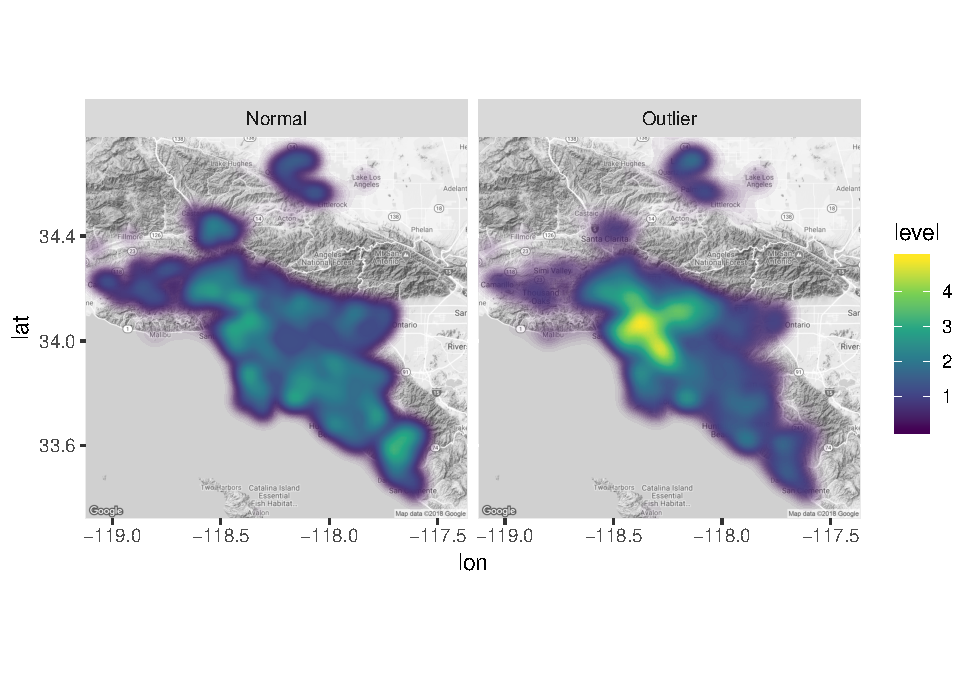
\includegraphics{zillow-prize_files/figure-latex/unnamed-chunk-5-1.pdf}
\caption{\label{fig:unnamed-chunk-5}Spatial Distribution of Log Error
Outliers}
\end{figure}

Now lets look at the spatiotemporal distribution of \texttt{log\_error}
outliers

\begin{Shaded}
\begin{Highlighting}[]
\NormalTok{trans_prop }\OperatorTok
\StringTok{  }\KeywordTok{filter}\NormalTok{(}
    \OperatorTok{!}\KeywordTok{is.na}\NormalTok{(lat),}
\NormalTok{    (}
\NormalTok{      log_error }\OperatorTok{<=}\StringTok{ }\KeywordTok{quantile}\NormalTok{(log_error, }\DataTypeTok{probs  =}\NormalTok{ .}\DecValTok{1}\NormalTok{) }\OperatorTok{|}\StringTok{ }
\StringTok{      }\NormalTok{log_error }\OperatorTok{>=}\StringTok{ }\KeywordTok{quantile}\NormalTok{(log_error, }\DataTypeTok{probs  =}\NormalTok{ .}\DecValTok{9}\NormalTok{)}
\NormalTok{      )}
\NormalTok{    ) }\OperatorTok
\StringTok{  }\KeywordTok{mutate}\NormalTok{(}
    \DataTypeTok{lon =} \KeywordTok{round}\NormalTok{(lon}\OperatorTok{/}\FloatTok{0.5}\NormalTok{, }\DataTypeTok{digits =} \DecValTok{1}\NormalTok{) }\OperatorTok{*}\StringTok{ }\FloatTok{0.5}\NormalTok{,}
    \DataTypeTok{lat =} \KeywordTok{round}\NormalTok{(lat}\OperatorTok{/}\FloatTok{0.5}\NormalTok{, }\DataTypeTok{digits =} \DecValTok{1}\NormalTok{) }\OperatorTok{*}\StringTok{ }\FloatTok{0.5}
\NormalTok{  ) }\OperatorTok
\StringTok{  }\KeywordTok{group_by}\NormalTok{(lon, lat, month_year) }\OperatorTok
\StringTok{  }\KeywordTok{summarise}\NormalTok{(}
    \DataTypeTok{n =} \KeywordTok{n}\NormalTok{()}
\NormalTok{  ) }\OperatorTok
\KeywordTok{ggplot}\NormalTok{(}\KeywordTok{aes}\NormalTok{(lon, lat)) }\OperatorTok{+}
\StringTok{  }\KeywordTok{geom_raster}\NormalTok{(}\KeywordTok{aes}\NormalTok{(}\DataTypeTok{fill =}\NormalTok{ n)) }\OperatorTok{+}
\StringTok{  }\KeywordTok{scale_fill_viridis_c}\NormalTok{() }\OperatorTok{+}
\StringTok{  }\KeywordTok{facet_wrap}\NormalTok{(}\OperatorTok{~}\NormalTok{month_year, }\DataTypeTok{ncol =} \DecValTok{3}\NormalTok{) }\OperatorTok{+}
\StringTok{  }\KeywordTok{coord_quickmap}\NormalTok{() }\OperatorTok{+}
\StringTok{  }\KeywordTok{theme_dark}\NormalTok{() }\OperatorTok{+}
\StringTok{  }\KeywordTok{labs}\NormalTok{(}
    \DataTypeTok{subtitle =} \StringTok{"Downtown Los Angeles looks to be consistently bad"}\NormalTok{,}
    \DataTypeTok{fill =} \StringTok{"Count"}
\NormalTok{  ) }\OperatorTok{+}
\StringTok{  }\KeywordTok{theme}\NormalTok{(}
    \DataTypeTok{axis.text =} \KeywordTok{element_text}\NormalTok{(}\DataTypeTok{size =} \DecValTok{5}\NormalTok{)}
\NormalTok{    )}
\end{Highlighting}
\end{Shaded}

\begin{figure}
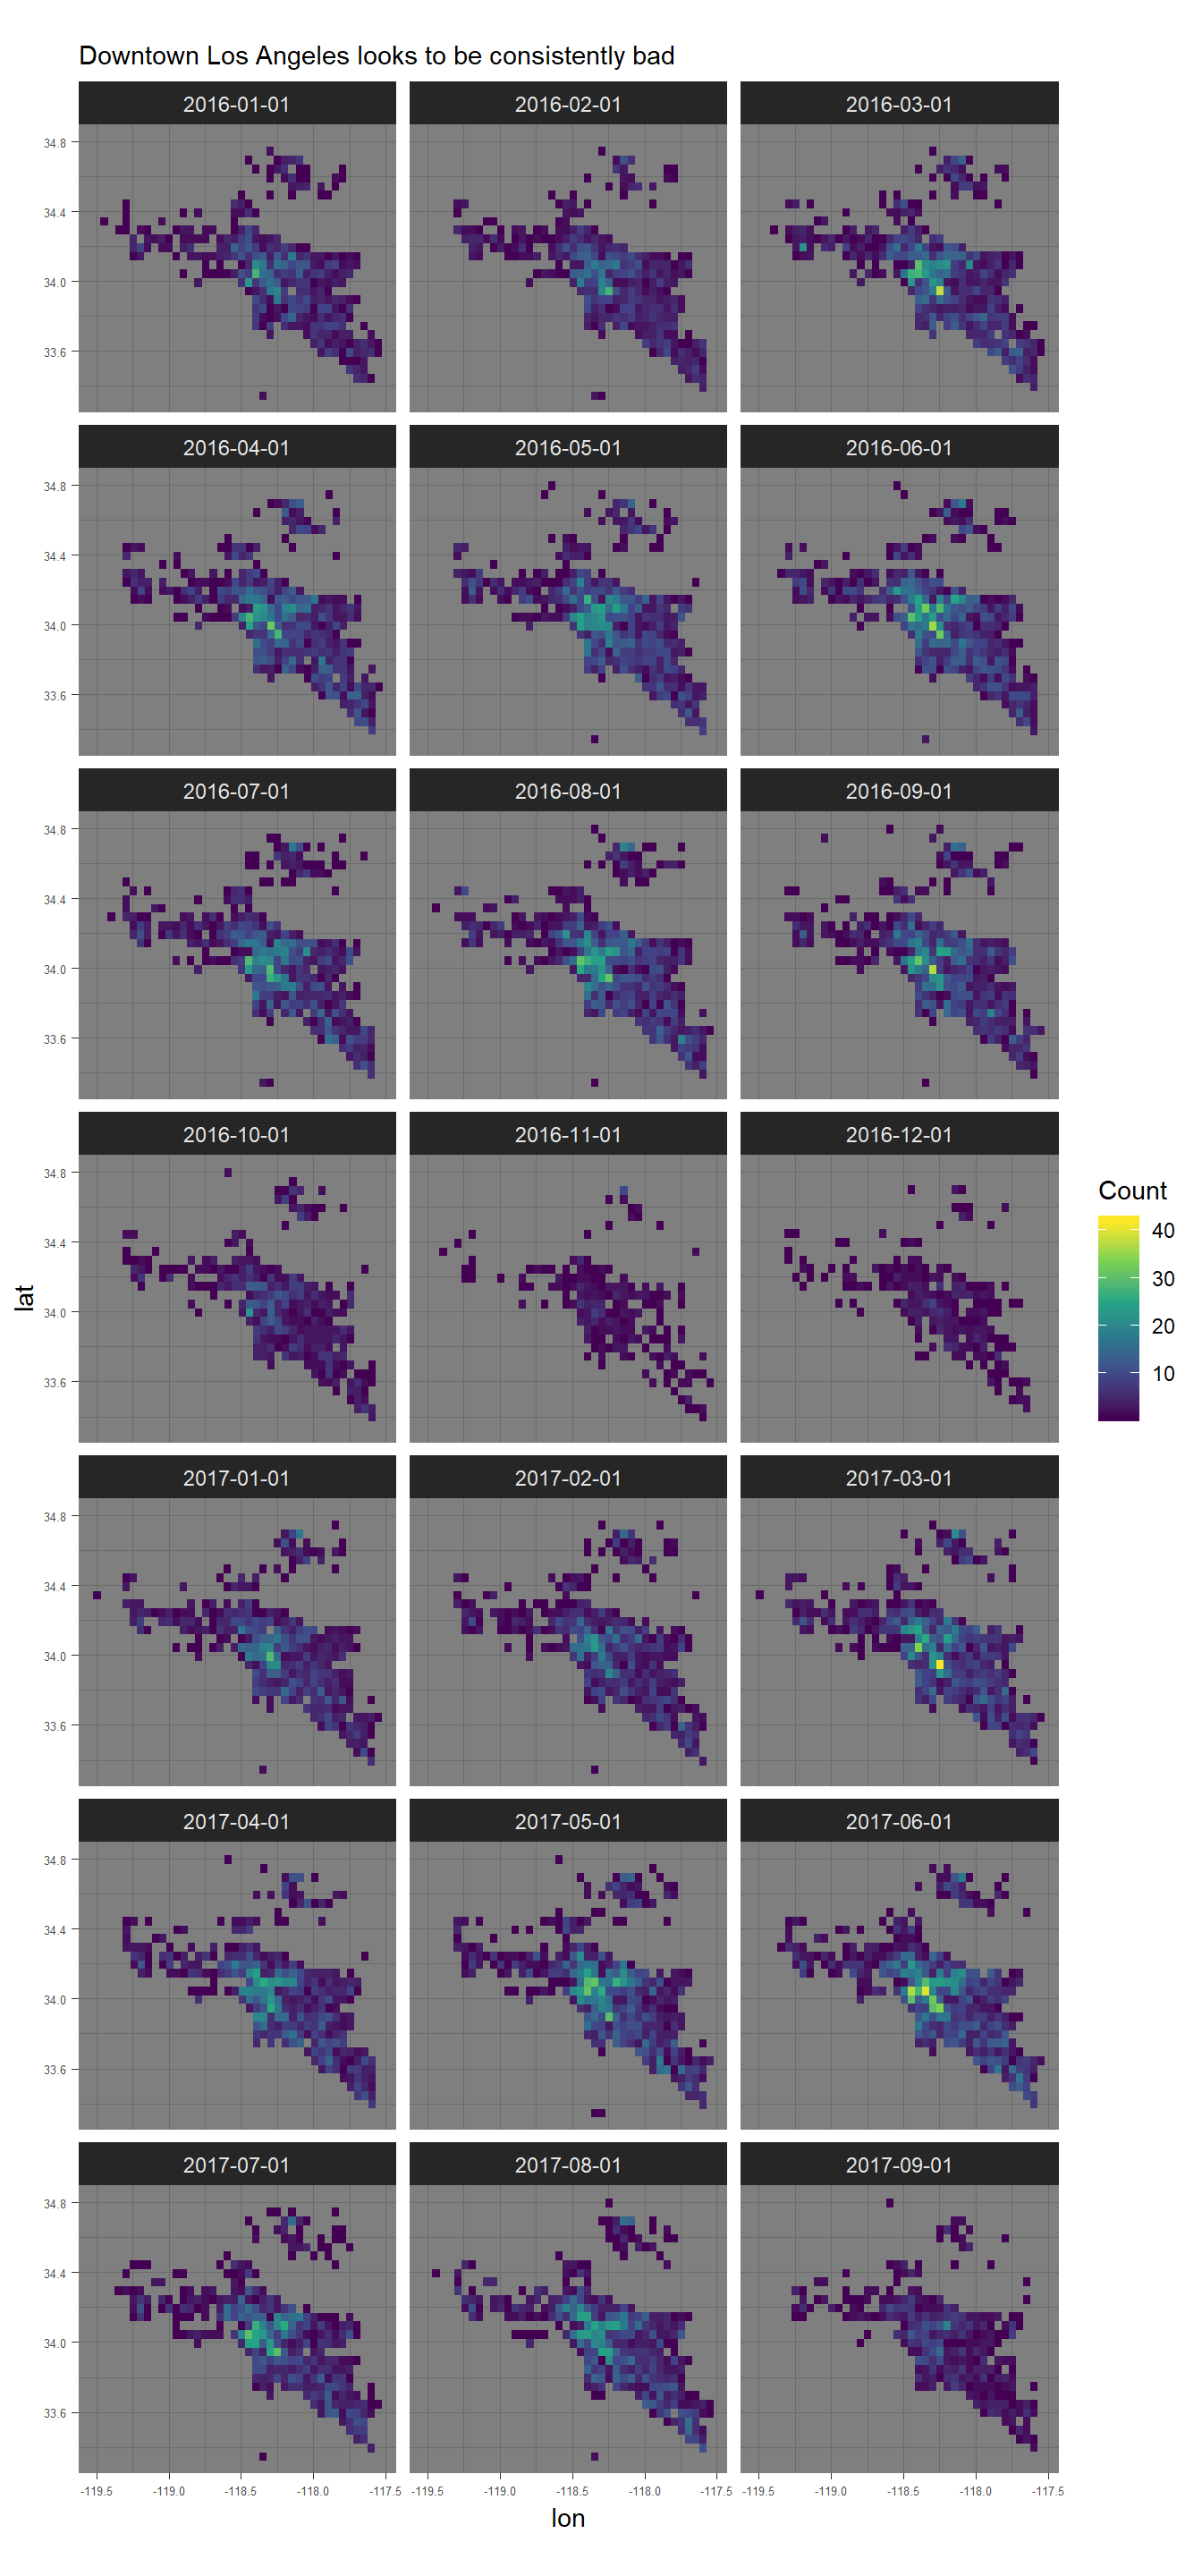
\includegraphics[width=1\linewidth]{zillow-prize_files/figure-latex/le-out-month-1} \caption{SpatioTemporal Distribution of Log Error Outliers}\label{fig:le-out-month}
\end{figure}

At first glance there looks to be a strong spatial and temporal
correlation to \texttt{log\_error}. Let's look more into the spatial
correlation.

Moran's I and its variant Local Moran's I, provide a useful measure of
the amount of spatial autocorrelation in a variable.

\begin{Shaded}
\begin{Highlighting}[]
\KeywordTok{library}\NormalTok{(spatstat)}
\KeywordTok{library}\NormalTok{(spdep)}

\NormalTok{d <-}\StringTok{ }\NormalTok{trans_prop }\OperatorTok
\StringTok{  }\KeywordTok{filter}\NormalTok{(}
    \OperatorTok{!}\KeywordTok{is.na}\NormalTok{(lat),}
\NormalTok{    (}
\NormalTok{      log_error }\OperatorTok{<=}\StringTok{ }\KeywordTok{quantile}\NormalTok{(log_error, }\DataTypeTok{probs  =}\NormalTok{ .}\DecValTok{1}\NormalTok{) }\OperatorTok{|}\StringTok{ }
\StringTok{      }\NormalTok{log_error }\OperatorTok{>=}\StringTok{ }\KeywordTok{quantile}\NormalTok{(log_error, }\DataTypeTok{probs  =}\NormalTok{ .}\DecValTok{9}\NormalTok{)}
\NormalTok{      )}
\NormalTok{    ) }\OperatorTok
\StringTok{  }\KeywordTok{mutate}\NormalTok{(}
    \DataTypeTok{lon =} \KeywordTok{round}\NormalTok{(lon}\OperatorTok{/}\FloatTok{0.1}\NormalTok{, }\DataTypeTok{digits =} \DecValTok{1}\NormalTok{) }\OperatorTok{*}\StringTok{ }\FloatTok{0.1}\NormalTok{,}
    \DataTypeTok{lat =} \KeywordTok{round}\NormalTok{(lat}\OperatorTok{/}\FloatTok{0.1}\NormalTok{, }\DataTypeTok{digits =} \DecValTok{1}\NormalTok{) }\OperatorTok{*}\StringTok{ }\FloatTok{0.1}
\NormalTok{  ) }\OperatorTok
\StringTok{  }\KeywordTok{group_by}\NormalTok{(lon, lat) }\OperatorTok
\StringTok{  }\KeywordTok{summarise}\NormalTok{(}
    \DataTypeTok{n =} \KeywordTok{n}\NormalTok{()}
\NormalTok{  )}

\KeywordTok{coordinates}\NormalTok{(d) <-}\StringTok{ }\ErrorTok{~}\NormalTok{lon }\OperatorTok{+}\StringTok{ }\NormalTok{lat}
\NormalTok{w <-}\StringTok{ }\KeywordTok{knn2nb}\NormalTok{(}\KeywordTok{knearneigh}\NormalTok{(d, }\DataTypeTok{k =} \DecValTok{10}\NormalTok{, }\DataTypeTok{longlat =} \OtherTok{TRUE}\NormalTok{))}
\KeywordTok{moran.test}\NormalTok{(d}\OperatorTok{$}\NormalTok{n, }\KeywordTok{nb2listw}\NormalTok{(w))}
\end{Highlighting}
\end{Shaded}

\begin{verbatim}
## 
##  Moran I test under randomisation
## 
## data:  d$n  
## weights: nb2listw(w)    
## 
## Moran I statistic standard deviate = 71.112, p-value < 2.2e-16
## alternative hypothesis: greater
## sample estimates:
## Moran I statistic       Expectation          Variance 
##      4.308120e-01     -1.952362e-04      3.673489e-05
\end{verbatim}

\begin{Shaded}
\begin{Highlighting}[]
\NormalTok{local_moran <-}\StringTok{ }\KeywordTok{as.data.frame}\NormalTok{(}\KeywordTok{localmoran}\NormalTok{(d}\OperatorTok{$}\NormalTok{n, }\KeywordTok{nb2listw}\NormalTok{(w)))}

\NormalTok{d }\OperatorTok
\StringTok{  }\KeywordTok{as.data.frame}\NormalTok{() }\OperatorTok
\StringTok{  }\KeywordTok{cbind}\NormalTok{(local_moran) }\OperatorTok
\StringTok{  }\KeywordTok{ggplot}\NormalTok{(}\KeywordTok{aes}\NormalTok{(lon, lat)) }\OperatorTok{+}
\StringTok{  }\KeywordTok{geom_raster}\NormalTok{(}\KeywordTok{aes}\NormalTok{(}\DataTypeTok{fill =}\NormalTok{ Ii)) }\OperatorTok{+}
\StringTok{  }\KeywordTok{scale_fill_viridis_c}\NormalTok{() }\OperatorTok{+}
\StringTok{  }\KeywordTok{coord_quickmap}\NormalTok{() }\OperatorTok{+}
\StringTok{  }\KeywordTok{theme_dark}\NormalTok{() }\OperatorTok{+}
\StringTok{  }\KeywordTok{labs}\NormalTok{(}
    \DataTypeTok{title =} \StringTok{"Local Moran's I on Outliers Density"}\NormalTok{,}
    \DataTypeTok{fill =} \StringTok{"Local Moran's I"}
\NormalTok{  )}
\end{Highlighting}
\end{Shaded}

\begin{figure}
\centering
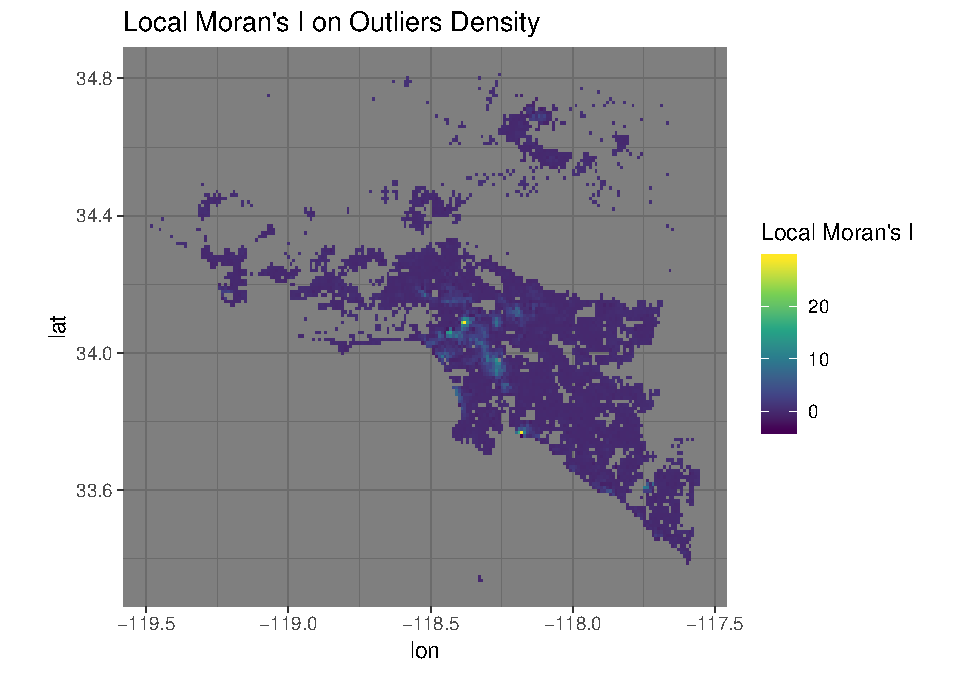
\includegraphics{zillow-prize_files/figure-latex/morans-i-outliers-1.pdf}
\caption{\label{fig:morans-i-outliers}Spatial Autocorrelation of Log Error
Outliers}
\end{figure}

Let's save our pared down \texttt{properties} table and then get into
feature engineering

\begin{Shaded}
\begin{Highlighting}[]
\KeywordTok{write_feather}\NormalTok{(properties, }\StringTok{"data/properties_17_filtered.feather"}\NormalTok{)}
\end{Highlighting}
\end{Shaded}

\chapter{Feature Engineering}\label{feat-eng}

After we have done an intital EDA of our data we can start doing some
feature engineering, this is where we can create new features such as
interaction variables, apply transformations such as centering and
scaling, choice how we want to encode our categorical features, and also
bring in new external information.

Just as in Chapter \ref{eda}, throughout this section we will
progressively updating our \texttt{properties} data to include new and
transformed features that we are going to continue with into the next
stages.

\section{Creating New Features}\label{creating-new-features}

\begin{quote}
``Everything is related to everything else, but near things are more
related than distant things.''

--- Waldo Tobler
\end{quote}

This ``First Law of Geography'' is something we can take advantage of
for creating new features based on our existing ones. In this section we
will create based on both data from the Kaggle competition and also
examples of external sources as well

\subsection{Internal Features}\label{internal-features}

Since we have the neighborhood, as defined by
\texttt{id\_geo\_bg\_fips}, that each parcel is apart of, we can use
this to create neighborhood average features.

There are many ways one could define neighborhood for the purposes of
using near by parcels, knn for example. Perhaps a more rigourous and
certainly more computationly intensive approach would be to estimate the
radius at which the spatial autocorrelation of \texttt{log\_error} is no
longer statistically significant using something such as a bootstrapped
spline correlogram such as the function \texttt{spline.correlog()}
provided by the \texttt{ncf} package

\begin{Shaded}
\begin{Highlighting}[]
\NormalTok{ncf}\OperatorTok{::}\KeywordTok{spline.correlog}\NormalTok{(}\DataTypeTok{x =}\NormalTok{ lon, }\DataTypeTok{y =}\NormalTok{ lat, }\DataTypeTok{z =}\NormalTok{ log_error)}
\end{Highlighting}
\end{Shaded}

For now we will stick with defining our neighborhood by the census block
group (\texttt{id\_geo\_bg\_fips}) that each parcel is apart of

\subsubsection{\texorpdfstring{Neigborhood Average \texttt{properties}
Features}{Neigborhood Average properties Features}}\label{neigborhood-average-properties-features}

\begin{Shaded}
\begin{Highlighting}[]
\NormalTok{bg_avg_features <-}\StringTok{ }\NormalTok{properties }\OperatorTok
\StringTok{  }\KeywordTok{group_by}\NormalTok{(id_geo_bg_fips) }\OperatorTok
\StringTok{  }\KeywordTok{select}\NormalTok{(}\OperatorTok{-}\NormalTok{id_parcel) }\OperatorTok
\StringTok{  }\KeywordTok{select_if}\NormalTok{(is.numeric) }\OperatorTok
\StringTok{  }\KeywordTok{summarise_all}\NormalTok{(mean, }\DataTypeTok{na.rm =} \OtherTok{TRUE}\NormalTok{) }\OperatorTok
\StringTok{  }\KeywordTok{filter}\NormalTok{(}
    \OperatorTok{!}\KeywordTok{is.na}\NormalTok{(id_geo_bg_fips)}
\NormalTok{    )}

\KeywordTok{names}\NormalTok{(bg_avg_features) <-}\StringTok{ }\KeywordTok{paste0}\NormalTok{(}\StringTok{"bg_avg_"}\NormalTok{, }\KeywordTok{names}\NormalTok{(bg_avg_features))}
\KeywordTok{names}\NormalTok{(bg_avg_features)[}\DecValTok{1}\NormalTok{] <-}\StringTok{ "id_geo_bg_fips"}

\CommentTok{# update the properties table}
\NormalTok{properties <-}\StringTok{ }\NormalTok{properties }\OperatorTok
\StringTok{  }\KeywordTok{left_join}\NormalTok{(bg_avg_features, }\DataTypeTok{by =} \StringTok{"id_geo_bg_fips"}\NormalTok{)}
\end{Highlighting}
\end{Shaded}

\subsubsection{\texorpdfstring{Rolling Local Average
\texttt{log\_error}}{Rolling Local Average log\_error}}\label{rolling-local-average-log_error}

There is a strong spatial and temporal autocorrelation to our response
variable \texttt{log\_error}. To take advantage of this, let's create a
few new features based on the rolling average of the local
\texttt{log\_error} values.

Because these features will have values for every day from
\texttt{min(trans\$date)} to \texttt{max(trans\$date)} we won't join
them to our data yet.

\begin{Shaded}
\begin{Highlighting}[]
\KeywordTok{library}\NormalTok{(tibbletime)}

\NormalTok{trans_prop <-}\StringTok{ }\NormalTok{properties_geo }\OperatorTok
\StringTok{  }\KeywordTok{right_join}\NormalTok{(trans, }\DataTypeTok{by =} \StringTok{"id_parcel"}\NormalTok{) }\OperatorTok
\StringTok{  }\KeywordTok{select}\NormalTok{(}
\NormalTok{    id_parcel,}
\NormalTok{    id_geo_bg_fips,}
\NormalTok{    id_geo_tract_fips,}
\NormalTok{    date,}
\NormalTok{    log_error}
\NormalTok{  )}

\CommentTok{# create rolling functions ------------------------------------------------}

\NormalTok{rolling_sum_}\DecValTok{7}\NormalTok{ <-}\StringTok{ }\KeywordTok{rollify}\NormalTok{(}\OperatorTok{~}\KeywordTok{sum}\NormalTok{(.x, }\DataTypeTok{na.rm =} \OtherTok{TRUE}\NormalTok{), }\DataTypeTok{window =} \DecValTok{7}\NormalTok{)}
\NormalTok{rolling_sum_}\DecValTok{28}\NormalTok{ <-}\StringTok{ }\KeywordTok{rollify}\NormalTok{(}\OperatorTok{~}\KeywordTok{sum}\NormalTok{(.x, }\DataTypeTok{na.rm =} \OtherTok{TRUE}\NormalTok{), }\DataTypeTok{window =} \DecValTok{28}\NormalTok{)}

\CommentTok{# by block group ----------------------------------------------------------}

\NormalTok{roll_bg <-}\StringTok{ }\KeywordTok{create_series}\NormalTok{(}\KeywordTok{min}\NormalTok{(trans_prop}\OperatorTok{$}\NormalTok{date) }\OperatorTok{~}\StringTok{ }\KeywordTok{max}\NormalTok{(trans_prop}\OperatorTok{$}\NormalTok{date), }
                   \StringTok{'daily'}\NormalTok{, }\DataTypeTok{class =} \StringTok{"Date"}\NormalTok{) }\OperatorTok
\StringTok{  }\NormalTok{tidyr}\OperatorTok{::}\KeywordTok{expand}\NormalTok{(}
\NormalTok{    date, }
    \DataTypeTok{id_geo_bg_fips =} \KeywordTok{unique}\NormalTok{(trans_prop}\OperatorTok{$}\NormalTok{id_geo_bg_fips)}
\NormalTok{  ) }\OperatorTok
\StringTok{  }\KeywordTok{full_join}\NormalTok{(trans_prop) }\OperatorTok
\StringTok{  }\KeywordTok{group_by}\NormalTok{(id_geo_bg_fips, date) }\OperatorTok
\StringTok{  }\KeywordTok{summarise}\NormalTok{(}
    \DataTypeTok{sum_log_error =} \KeywordTok{sum}\NormalTok{(log_error, }\DataTypeTok{na.rm =} \OtherTok{TRUE}\NormalTok{),}
    \DataTypeTok{sales_total =} \KeywordTok{sum}\NormalTok{(}\OperatorTok{!}\KeywordTok{is.na}\NormalTok{(log_error))}
\NormalTok{    ) }\OperatorTok
\StringTok{  }\KeywordTok{ungroup}\NormalTok{() }\OperatorTok\StringTok{ }
\StringTok{  }\KeywordTok{group_by}\NormalTok{(id_geo_bg_fips) }\OperatorTok
\StringTok{  }\KeywordTok{mutate}\NormalTok{(}
    \DataTypeTok{sum_log_error_7days =} \KeywordTok{rolling_sum_7}\NormalTok{(sum_log_error),}
    \DataTypeTok{sum_log_error_28days  =}  \KeywordTok{rolling_sum_28}\NormalTok{(sum_log_error),}
    \DataTypeTok{roll_bg_trans_total_7days =} \KeywordTok{rolling_sum_7}\NormalTok{(sales_total),}
    \DataTypeTok{roll_bg_trans_total_28days  =}  \KeywordTok{rolling_sum_28}\NormalTok{(sales_total),}
    \DataTypeTok{roll_bg_avg_log_error_7days =}\NormalTok{ sum_log_error_7days }\OperatorTok{/}\StringTok{ }\NormalTok{roll_bg_trans_total_7days,}
    \DataTypeTok{roll_bg_avg_log_error_28days =}\NormalTok{ sum_log_error_28days }\OperatorTok{/}\StringTok{ }\NormalTok{roll_bg_trans_total_28days,}
    \DataTypeTok{date =}\NormalTok{ date }\OperatorTok{+}\StringTok{ }\NormalTok{lubridate}\OperatorTok{::}\KeywordTok{days}\NormalTok{(}\DecValTok{1}\NormalTok{) }\CommentTok{# to not include the current day in avg}
\NormalTok{  ) }\OperatorTok
\StringTok{  }\KeywordTok{select}\NormalTok{(}
\NormalTok{    id_geo_bg_fips,}
\NormalTok{    date,}
\NormalTok{    roll_bg_trans_total_7days,}
\NormalTok{    roll_bg_trans_total_28days,}
\NormalTok{    roll_bg_avg_log_error_7days,}
\NormalTok{    roll_bg_avg_log_error_28days}
\NormalTok{  ) }\OperatorTok
\StringTok{  }\KeywordTok{mutate}\NormalTok{(}
    \DataTypeTok{roll_bg_trans_total_7days =} \KeywordTok{ifelse}\NormalTok{(}\KeywordTok{is.na}\NormalTok{(roll_bg_trans_total_7days), }
                                       \DecValTok{0}\NormalTok{, roll_bg_trans_total_7days),}
    \DataTypeTok{roll_bg_trans_total_28days =} \KeywordTok{ifelse}\NormalTok{(}\KeywordTok{is.na}\NormalTok{(roll_bg_trans_total_28days), }
                                        \DecValTok{0}\NormalTok{, roll_bg_trans_total_28days),}
    \DataTypeTok{roll_bg_avg_log_error_7days =} \KeywordTok{ifelse}\NormalTok{(}\KeywordTok{is.nan}\NormalTok{(roll_bg_avg_log_error_7days), }
                                         \DecValTok{0}\NormalTok{, roll_bg_avg_log_error_7days),}
    \DataTypeTok{roll_bg_avg_log_error_28days =} \KeywordTok{ifelse}\NormalTok{(}\KeywordTok{is.nan}\NormalTok{(roll_bg_avg_log_error_28days), }
                                          \DecValTok{0}\NormalTok{, roll_bg_avg_log_error_28days),}
    \DataTypeTok{roll_bg_avg_log_error_7days =} \KeywordTok{as.numeric}\NormalTok{(forecast}\OperatorTok{::}\KeywordTok{na.interp}\NormalTok{(roll_bg_avg_log_error_7days)),}
    \DataTypeTok{roll_bg_avg_log_error_28days =} \KeywordTok{as.numeric}\NormalTok{(forecast}\OperatorTok{::}\KeywordTok{na.interp}\NormalTok{(roll_bg_avg_log_error_28days))}
\NormalTok{  )}

\CommentTok{# by tract ----------------------------------------------------------------}

\NormalTok{roll_tract <-}\StringTok{ }\KeywordTok{create_series}\NormalTok{(}\KeywordTok{min}\NormalTok{(trans_prop}\OperatorTok{$}\NormalTok{date) }\OperatorTok{~}\StringTok{ }\KeywordTok{max}\NormalTok{(trans_prop}\OperatorTok{$}\NormalTok{date), }
                         \StringTok{'daily'}\NormalTok{, }\DataTypeTok{class =} \StringTok{"Date"}\NormalTok{) }\OperatorTok
\StringTok{  }\NormalTok{tidyr}\OperatorTok{::}\KeywordTok{expand}\NormalTok{(}
\NormalTok{    date, }
    \DataTypeTok{id_geo_tract_fips =} \KeywordTok{unique}\NormalTok{(trans_prop}\OperatorTok{$}\NormalTok{id_geo_tract_fips)}
\NormalTok{  ) }\OperatorTok
\StringTok{  }\KeywordTok{full_join}\NormalTok{(trans_prop) }\OperatorTok
\StringTok{  }\KeywordTok{group_by}\NormalTok{(id_geo_tract_fips, date) }\OperatorTok
\StringTok{  }\KeywordTok{summarise}\NormalTok{(}
    \DataTypeTok{sum_log_error =} \KeywordTok{sum}\NormalTok{(log_error, }\DataTypeTok{na.rm =} \OtherTok{TRUE}\NormalTok{),}
    \DataTypeTok{sales_total =} \KeywordTok{sum}\NormalTok{(}\OperatorTok{!}\KeywordTok{is.na}\NormalTok{(log_error))}
\NormalTok{  ) }\OperatorTok
\StringTok{  }\KeywordTok{ungroup}\NormalTok{() }\OperatorTok\StringTok{ }
\StringTok{  }\KeywordTok{group_by}\NormalTok{(id_geo_tract_fips) }\OperatorTok
\StringTok{  }\KeywordTok{mutate}\NormalTok{(}
    \DataTypeTok{sum_log_error_7days =} \KeywordTok{rolling_sum_7}\NormalTok{(sum_log_error),}
    \DataTypeTok{sum_log_error_28days  =}  \KeywordTok{rolling_sum_28}\NormalTok{(sum_log_error),}
    \DataTypeTok{roll_tract_trans_total_7days =} \KeywordTok{rolling_sum_7}\NormalTok{(sales_total),}
    \DataTypeTok{roll_tract_trans_total_28days  =}  \KeywordTok{rolling_sum_28}\NormalTok{(sales_total),}
    \DataTypeTok{roll_tract_avg_log_error_7days =}\NormalTok{ sum_log_error_7days }\OperatorTok{/}\StringTok{ }\NormalTok{roll_tract_trans_total_7days,}
    \DataTypeTok{roll_tract_avg_log_error_28days =}\NormalTok{ sum_log_error_28days }\OperatorTok{/}\StringTok{ }\NormalTok{roll_tract_trans_total_28days,}
    \DataTypeTok{date =}\NormalTok{ date }\OperatorTok{+}\StringTok{ }\NormalTok{lubridate}\OperatorTok{::}\KeywordTok{days}\NormalTok{(}\DecValTok{1}\NormalTok{) }\CommentTok{# to not include the current day in avg}
\NormalTok{  ) }\OperatorTok
\StringTok{  }\KeywordTok{select}\NormalTok{(}
\NormalTok{    id_geo_tract_fips,}
\NormalTok{    date,}
\NormalTok{    roll_tract_trans_total_7days,}
\NormalTok{    roll_tract_trans_total_28days,}
\NormalTok{    roll_tract_avg_log_error_7days,}
\NormalTok{    roll_tract_avg_log_error_28days}
\NormalTok{  ) }\OperatorTok
\StringTok{  }\KeywordTok{mutate}\NormalTok{(}
    \DataTypeTok{roll_tract_trans_total_7days =} \KeywordTok{ifelse}\NormalTok{(}\KeywordTok{is.na}\NormalTok{(roll_tract_trans_total_7days), }
                                          \DecValTok{0}\NormalTok{, roll_tract_trans_total_7days),}
    \DataTypeTok{roll_tract_trans_total_28days =} \KeywordTok{ifelse}\NormalTok{(}\KeywordTok{is.na}\NormalTok{(roll_tract_trans_total_28days), }
                                           \DecValTok{0}\NormalTok{, roll_tract_trans_total_28days),}
    \DataTypeTok{roll_tract_avg_log_error_7days =} \KeywordTok{ifelse}\NormalTok{(}\KeywordTok{is.nan}\NormalTok{(roll_tract_avg_log_error_7days), }
                                            \DecValTok{0}\NormalTok{, roll_tract_avg_log_error_7days),}
    \DataTypeTok{roll_tract_avg_log_error_28days =} \KeywordTok{ifelse}\NormalTok{(}\KeywordTok{is.nan}\NormalTok{(roll_tract_avg_log_error_28days), }
                                             \DecValTok{0}\NormalTok{, roll_tract_avg_log_error_28days),}
    \DataTypeTok{roll_tract_avg_log_error_7days =} \KeywordTok{as.numeric}\NormalTok{(forecast}\OperatorTok{::}\KeywordTok{na.interp}\NormalTok{(roll_tract_avg_log_error_7days)),}
    \DataTypeTok{roll_tract_avg_log_error_28days =} \KeywordTok{as.numeric}\NormalTok{(forecast}\OperatorTok{::}\KeywordTok{na.interp}\NormalTok{(roll_tract_avg_log_error_28days))}
\NormalTok{  )}

\NormalTok{prop_geo_ids <-}\StringTok{ }\NormalTok{properties_geo }\OperatorTok
\StringTok{  }\KeywordTok{select}\NormalTok{(}
\NormalTok{    id_parcel,}
\NormalTok{    id_geo_bg_fips,}
\NormalTok{    id_geo_tract_fips}
\NormalTok{  )}

\KeywordTok{write_feather}\NormalTok{(roll_bg, }\StringTok{"data/external-features/roll_features_blockgroup.feather"}\NormalTok{)}
\KeywordTok{write_feather}\NormalTok{(roll_tract, }\StringTok{"data/external-features/roll_features_tract.feather"}\NormalTok{)}
\end{Highlighting}
\end{Shaded}

\subsection{External Features}\label{external-features}

Breaking from the rules of the actual Kaggle competition, we're going to
add in some external features as an example of bringing in other
information

\subsubsection{American Community
Survey}\label{american-community-survey}

The \href{https://www.census.gov/programs-surveys/acs/}{American
Community Survey} is a great source of demographic and household data.
As an example of using this data let's bring in a few features related
to our area of interest.

In our example here, we are completely ignoring the margin or error for
each feature, given more time investigating the information contained in
these fields is most likely worth your while.

There are literally thousands you can explore in the ACS. For our
example, we are going to use a few

\begin{Shaded}
\begin{Highlighting}[]
\KeywordTok{library}\NormalTok{(tidycensus)}

\NormalTok{api_key <-}\StringTok{ }\KeywordTok{Sys.getenv}\NormalTok{(}\StringTok{"CENSUS_API_KEY"}\NormalTok{)}
\KeywordTok{census_api_key}\NormalTok{(api_key)}

\NormalTok{acs_var_list <-}\StringTok{ }\KeywordTok{load_variables}\NormalTok{(}\DecValTok{2016}\NormalTok{, }\StringTok{"acs5"}\NormalTok{, }\DataTypeTok{cache =} \OtherTok{TRUE}\NormalTok{)}

\NormalTok{acs_bg_vars <-}\StringTok{ }\KeywordTok{c}\NormalTok{(}\StringTok{"B25034_001E"}\NormalTok{, }\StringTok{"B25034_002E"}\NormalTok{, }\StringTok{"B25034_003E"}\NormalTok{, }
                 \StringTok{"B25034_004E"}\NormalTok{, }\StringTok{"B25034_005E"}\NormalTok{, }\StringTok{"B25034_006E"}\NormalTok{,}
                 \StringTok{"B25034_007E"}\NormalTok{, }\StringTok{"B25034_008E"}\NormalTok{, }\StringTok{"B25034_009E"}\NormalTok{,}
                 \StringTok{"B25034_010E"}\NormalTok{, }\StringTok{"B25034_011E"}\NormalTok{, }\StringTok{"B25076_001E"}\NormalTok{, }
                 \StringTok{"B25077_001E"}\NormalTok{, }\StringTok{"B25078_001E"}\NormalTok{, }\StringTok{"B25056_001E"}\NormalTok{, }
                 \StringTok{"B25002_001E"}\NormalTok{, }\StringTok{"B25002_003E"}\NormalTok{, }\StringTok{"B25001_001E"}\NormalTok{)}

\NormalTok{acs_bg_home_value <-}\StringTok{ }\NormalTok{acs_var_list }\OperatorTok
\StringTok{  }\KeywordTok{filter}\NormalTok{(}\KeywordTok{grepl}\NormalTok{(}\StringTok{"B25075_"}\NormalTok{, }\DataTypeTok{x =}\NormalTok{ name))}

\NormalTok{acs_bg_home_value_vars <-}\StringTok{ }\NormalTok{acs_bg_home_value}\OperatorTok{$}\NormalTok{name}

\NormalTok{acs_bg_vars <-}\StringTok{ }\KeywordTok{c}\NormalTok{(acs_bg_vars, acs_bg_home_value_vars)}

\NormalTok{acs_bg_data <-}\StringTok{ }\KeywordTok{get_acs}\NormalTok{(}
  \DataTypeTok{geography =} \StringTok{"block group"}\NormalTok{, }
  \DataTypeTok{variables =}\NormalTok{ acs_bg_vars, }
  \DataTypeTok{state =} \StringTok{"CA"}\NormalTok{,}
  \DataTypeTok{county =} \KeywordTok{c}\NormalTok{(}\StringTok{"Los Angeles"}\NormalTok{, }\StringTok{"Orange"}\NormalTok{, }\StringTok{"Ventura"}\NormalTok{),}
  \DataTypeTok{output =} \StringTok{"wide"}\NormalTok{,}
  \DataTypeTok{geometry =} \OtherTok{FALSE}\NormalTok{, }
  \DataTypeTok{keep_geo_vars =} \OtherTok{TRUE}
\NormalTok{)}

\NormalTok{acs_bg_data1 <-}\StringTok{ }\NormalTok{acs_bg_data }\OperatorTok
\StringTok{  }\KeywordTok{select}\NormalTok{(}
    \DataTypeTok{id_geo_bg_fips =}\NormalTok{ GEOID,}
    \DataTypeTok{acs_str_yr_total =}\NormalTok{ B25034_001E,}
    \DataTypeTok{acs_str_yr_2014_later =}\NormalTok{ B25034_002E,}
    \DataTypeTok{acs_str_yr_2010_2013 =}\NormalTok{ B25034_003E,}
    \DataTypeTok{acs_str_yr_2000_2009 =}\NormalTok{ B25034_004E,}
    \DataTypeTok{acs_str_yr_1990_1999 =}\NormalTok{ B25034_005E,}
    \DataTypeTok{acs_str_yr_1980_1989 =}\NormalTok{ B25034_006E,}
    \DataTypeTok{acs_str_yr_1970_1979 =}\NormalTok{ B25034_007E,}
    \DataTypeTok{acs_str_yr_1960_1969 =}\NormalTok{ B25034_008E,}
    \DataTypeTok{acs_str_yr_1950_1959 =}\NormalTok{ B25034_009E,}
    \DataTypeTok{acs_str_yr_1940_1949 =}\NormalTok{ B25034_010E,}
    \DataTypeTok{acs_str_yr_1939_earlier =}\NormalTok{ B25034_011E,}
    \DataTypeTok{acs_home_value_lwr =}\NormalTok{ B25076_001E,}
    \DataTypeTok{acs_home_value_med =}\NormalTok{ B25077_001E,}
    \DataTypeTok{acs_home_value_upr =}\NormalTok{ B25078_001E,}
    \DataTypeTok{acs_num_of_renters_total =}\NormalTok{ B25056_001E,}
    \DataTypeTok{acs_num_of_house_units =}\NormalTok{ B25001_001E,}
    \DataTypeTok{acs_occ_status_total =}\NormalTok{ B25002_001E,}
    \DataTypeTok{acs_occ_status_vacant =}\NormalTok{ B25002_003E,}
    \DataTypeTok{acs_home_value_cnt_total =}\NormalTok{ B25075_001E,}
    \DataTypeTok{acs_home_value_cnt_less_10k =}\NormalTok{ B25075_002E,}
    \DataTypeTok{acs_home_value_cnt_10k_15k =}\NormalTok{ B25075_003E,}
    \DataTypeTok{acs_home_value_cnt_15k_20k =}\NormalTok{ B25075_004E,}
    \DataTypeTok{acs_home_value_cnt_20k_25k =}\NormalTok{ B25075_005E,}
    \DataTypeTok{acs_home_value_cnt_25k_30k =}\NormalTok{ B25075_006E,}
    \DataTypeTok{acs_home_value_cnt_30k_35k =}\NormalTok{ B25075_007E,}
    \DataTypeTok{acs_home_value_cnt_35k_40k =}\NormalTok{ B25075_008E,}
    \DataTypeTok{acs_home_value_cnt_40k_50k =}\NormalTok{ B25075_009E,}
    \DataTypeTok{acs_home_value_cnt_50k_60k =}\NormalTok{ B25075_010E,}
    \DataTypeTok{acs_home_value_cnt_60k_70k =}\NormalTok{ B25075_011E,}
    \DataTypeTok{acs_home_value_cnt_70k_80k =}\NormalTok{ B25075_012E,}
    \DataTypeTok{acs_home_value_cnt_80k_90k =}\NormalTok{ B25075_013E,}
    \DataTypeTok{acs_home_value_cnt_90k_100k =}\NormalTok{ B25075_014E,}
    \DataTypeTok{acs_home_value_cnt_100k_125k =}\NormalTok{ B25075_015E,}
    \DataTypeTok{acs_home_value_cnt_125k_150k =}\NormalTok{ B25075_016E,}
    \DataTypeTok{acs_home_value_cnt_150k_175k =}\NormalTok{ B25075_017E,}
    \DataTypeTok{acs_home_value_cnt_175k_200k =}\NormalTok{ B25075_018E,}
    \DataTypeTok{acs_home_value_cnt_200k_250k =}\NormalTok{ B25075_019E,}
    \DataTypeTok{acs_home_value_cnt_250k_300k =}\NormalTok{ B25075_020E,}
    \DataTypeTok{acs_home_value_cnt_300k_400k =}\NormalTok{ B25075_021E,}
    \DataTypeTok{acs_home_value_cnt_400k_500k =}\NormalTok{ B25075_022E,}
    \DataTypeTok{acs_home_value_cnt_500k_750k =}\NormalTok{ B25075_023E,}
    \DataTypeTok{acs_home_value_cnt_750k_1000k =}\NormalTok{ B25075_024E,}
    \DataTypeTok{acs_home_value_cnt_1000k_1500k =}\NormalTok{ B25075_025E,}
    \DataTypeTok{acs_home_value_cnt_1500k_2000k =}\NormalTok{ B25075_026E,}
    \DataTypeTok{acs_home_value_cnt_2000k_more =}\NormalTok{ B25075_027E}
\NormalTok{  ) }\OperatorTok
\StringTok{  }\KeywordTok{mutate_at}\NormalTok{(}
    \KeywordTok{vars}\NormalTok{(}\KeywordTok{starts_with}\NormalTok{(}\StringTok{"acs_home_value_cnt"}\NormalTok{)), }\ControlFlowTok{function}\NormalTok{(x) }\KeywordTok{round}\NormalTok{(x }\OperatorTok{/}\StringTok{ }\NormalTok{.}\OperatorTok{$}\NormalTok{acs_home_value_cnt_total, }\DataTypeTok{digits =} \DecValTok{5}\NormalTok{)}
\NormalTok{    ) }\OperatorTok
\StringTok{  }\KeywordTok{mutate_at}\NormalTok{(}
    \KeywordTok{vars}\NormalTok{(}\KeywordTok{starts_with}\NormalTok{(}\StringTok{"acs_str_yr"}\NormalTok{)), }\ControlFlowTok{function}\NormalTok{(x) }\KeywordTok{round}\NormalTok{(x }\OperatorTok{/}\StringTok{ }\NormalTok{.}\OperatorTok{$}\NormalTok{acs_str_yr_total, }\DataTypeTok{digits =} \DecValTok{5}\NormalTok{)}
\NormalTok{  ) }\OperatorTok
\StringTok{  }\KeywordTok{mutate}\NormalTok{(}
    \DataTypeTok{acs_per_renters =} \KeywordTok{round}\NormalTok{(acs_num_of_renters_total }\OperatorTok{/}\StringTok{ }\NormalTok{acs_num_of_house_units, }\DataTypeTok{digits =} \DecValTok{5}\NormalTok{),}
    \DataTypeTok{acs_per_vacant =} \KeywordTok{round}\NormalTok{(acs_occ_status_vacant }\OperatorTok{/}\StringTok{ }\NormalTok{acs_occ_status_total, }\DataTypeTok{digits =} \DecValTok{5}\NormalTok{)}
\NormalTok{  ) }\OperatorTok
\StringTok{  }\KeywordTok{select}\NormalTok{(}
    \OperatorTok{-}\NormalTok{acs_occ_status_total, }
    \OperatorTok{-}\NormalTok{acs_home_value_cnt_total, }
    \OperatorTok{-}\NormalTok{acs_str_yr_total}
\NormalTok{    )}

\NormalTok{acs_features <-}\StringTok{ }\NormalTok{properties_geo }\OperatorTok
\StringTok{  }\KeywordTok{select}\NormalTok{(}
\NormalTok{    id_parcel,}
\NormalTok{    id_geo_bg_fips}
\NormalTok{    ) }\OperatorTok
\StringTok{  }\KeywordTok{left_join}\NormalTok{(acs_bg_data1, }\DataTypeTok{by =} \StringTok{"id_geo_bg_fips"}\NormalTok{) }\OperatorTok
\StringTok{  }\KeywordTok{select}\NormalTok{(}\OperatorTok{-}\NormalTok{id_geo_bg_fips)}

\NormalTok{properties <-}\StringTok{ }\NormalTok{properties }\OperatorTok
\StringTok{  }\KeywordTok{left_join}\NormalTok{(acs_features, }\DataTypeTok{by =} \StringTok{"id_parcel"}\NormalTok{)}
\end{Highlighting}
\end{Shaded}

\subsubsection{Economic Indicators}\label{economic-indicators}

The value of a home is not only influenced by itself and its neighbors,
but also larger economic trends. To help account for this in our model
we are going to add in the following economic indicators

\begin{itemize}
\tightlist
\item
  \href{https://fred.stlouisfed.org/series/MORTGAGE30US}{30-Year Fixed
  Rate Mortgage Average in the United States}
\item
  \href{https://fred.stlouisfed.org/series/LXXRSA}{S\&P/Case-Shiller
  CA-Los Angeles Home Price Index}
\item
  \href{https://fred.stlouisfed.org/series/CALOSA7URN}{Unemployment Rate
  in Los Angeles County, CA}
\end{itemize}

\begin{Shaded}
\begin{Highlighting}[]
\KeywordTok{library}\NormalTok{(alfred)}

\CommentTok{# 30-Year Fixed Rate Mortgage Average in the United States (weekly)}
\NormalTok{mort30 <-}\StringTok{ }\KeywordTok{get_fred_series}\NormalTok{(}\StringTok{"MORTGAGE30US"}\NormalTok{) }\OperatorTok\StringTok{ }
\StringTok{  }\KeywordTok{mutate}\NormalTok{(}
    \DataTypeTok{date_month =} \KeywordTok{floor_date}\NormalTok{(date, }\DataTypeTok{unit =} \StringTok{"month"}\NormalTok{),}
    \DataTypeTok{date_week =} \KeywordTok{floor_date}\NormalTok{(date, }\DataTypeTok{unit =} \StringTok{"week"}\NormalTok{)}
\NormalTok{    )}

\CommentTok{# S&P/Case-Shiller CA-Los Angeles Home Price Index (monthly)}
\NormalTok{spcs <-}\StringTok{ }\KeywordTok{get_fred_series}\NormalTok{(}\StringTok{"LXXRNSA"}\NormalTok{)}

\CommentTok{# Unemployment Rate in Los Angeles County, CA (monthly)}
\NormalTok{unemployment <-}\StringTok{ }\KeywordTok{get_fred_series}\NormalTok{(}\StringTok{"CALOSA7URN"}\NormalTok{)}

\NormalTok{econ_features <-}\StringTok{ }\KeywordTok{create_series}\NormalTok{(}\KeywordTok{min}\NormalTok{(mort30}\OperatorTok{$}\NormalTok{date) }\OperatorTok{~}\StringTok{ }\KeywordTok{max}\NormalTok{(mort30}\OperatorTok{$}\NormalTok{date), }
                               \StringTok{'daily'}\NormalTok{, }\DataTypeTok{class =} \StringTok{"Date"}\NormalTok{) }\OperatorTok
\StringTok{  }\KeywordTok{mutate}\NormalTok{(}\DataTypeTok{date_week =} \KeywordTok{floor_date}\NormalTok{(date, }\DataTypeTok{unit =} \StringTok{"week"}\NormalTok{)) }\OperatorTok
\StringTok{  }\KeywordTok{left_join}\NormalTok{(mort30, }\DataTypeTok{by =} \KeywordTok{c}\NormalTok{(}\StringTok{"date_week"}\NormalTok{ =}\StringTok{ "date_week"}\NormalTok{)) }\OperatorTok
\StringTok{  }\KeywordTok{left_join}\NormalTok{(spcs, }\DataTypeTok{by =} \KeywordTok{c}\NormalTok{(}\StringTok{"date_month"}\NormalTok{ =}\StringTok{ "date"}\NormalTok{)) }\OperatorTok
\StringTok{  }\KeywordTok{left_join}\NormalTok{(unemployment, }\DataTypeTok{by =} \KeywordTok{c}\NormalTok{(}\StringTok{"date_month"}\NormalTok{ =}\StringTok{ "date"}\NormalTok{)) }\OperatorTok
\StringTok{  }\KeywordTok{select}\NormalTok{(}
    \DataTypeTok{date =}\NormalTok{ date.x,}
    \DataTypeTok{econ_mort_30 =}\NormalTok{ MORTGAGE30US,}
    \DataTypeTok{econ_case_shiller =}\NormalTok{ LXXRNSA,}
    \DataTypeTok{econ_unemployment =}\NormalTok{ CALOSA7URN}
\NormalTok{  ) }\OperatorTok
\StringTok{  }\KeywordTok{filter}\NormalTok{(}
\NormalTok{    date }\OperatorTok{>=}\StringTok{ }\KeywordTok{date}\NormalTok{(}\StringTok{"2015-12-01"}\NormalTok{),}
\NormalTok{    date }\OperatorTok{<=}\StringTok{ }\KeywordTok{date}\NormalTok{(}\StringTok{"2018-01-01"}\NormalTok{)}
\NormalTok{    )}

\KeywordTok{write_feather}\NormalTok{(econ_features, }\StringTok{"data/external-features/econ_features.feather"}\NormalTok{)}
\end{Highlighting}
\end{Shaded}

Ok, so a check in on where we are. We currently have 5 data frames of
interest, our old friends \texttt{properties} which now contains new
features from our \texttt{bg\_avg\_features} neighborhood data and the
\texttt{acs\_features} which contain a few indicators from the American
Community Survey and \texttt{trans} which contains our response variable
\texttt{log\_error} as well as the transaction date and a few date based
features.

The other 3 data frames we have are seperated from the
\texttt{properties} and \texttt{trans} data currently because they
contain features that have different values for each day and depending
on what our transaction dates are for the partiuclar set of observations
we will use filter those values down and join them at the time of
training.

\section{Handling Missing Data}\label{handling-missing-data}

There are many ways to handle missing data from simple mean or median
imputation to more complex methods such as knn or multiple imputation or
even constructing other predictive models for predicting missing
features. We will not explore that topic in depth here and use a
somewhat simple approach that takes advantage of the spatial
relationships of our data.

We will use median (or modal for nominal features) imputation but
instead of doing global median values for all observations, we are going
to break our observations into subspaces based on
\texttt{zoning\_landuse}, \texttt{area\_lot}, and increasingly larger
neigborhood windows. The reasoning behind this choice is that the values
for many of the other features can vary widely across these categories.
For example it wouldn't make sense to include the \texttt{tax\_building}
values for mobile homes if we are imputing the \texttt{tax\_building}
value of a commercial office building. The is true for
\texttt{area\_lot} the tax burden on a large commercial office will be
larger then the one of a smaller office.

So we will look at increaingly larger neighborhoods of
\texttt{zoning\_landuse} and (a discretized version of)
\texttt{area\_lot} combinations, if there are any none \texttt{NA}
observations of that combination in the missing observations block
group, fill its values with the block group median (mode), if there are
no non-missing observations with that combination in that block group,
then look at the tract level, if there are none at the tract look at the
county level, and finally if there are no non-missing observations in
the County that the parcel belongs to, an unlikely event, then use the
``global'' values to impute.

To do this we first need to impute the values for
\texttt{zoning\_landuse} and \texttt{area\_lot}. For this we will just
use the increasing neighborhood search for \texttt{zoning\_landuse} and
then use the increasing neighborhood search broken down by
\texttt{zoning\_landuse} to fill in \texttt{area\_lot}

For some reason their are no built in functions for calculating the
mode. Make a simple helper function to do so

\begin{Shaded}
\begin{Highlighting}[]
\CommentTok{# simple helper function to find the mode}
\NormalTok{fct_mode <-}\StringTok{ }\ControlFlowTok{function}\NormalTok{(f) \{}
  
\NormalTok{  f_no_na <-}\StringTok{ }\KeywordTok{na.omit}\NormalTok{(f)}
\NormalTok{  fct_tab <-}\StringTok{ }\KeywordTok{table}\NormalTok{(f_no_na)}
  
  \CommentTok{# if everything NA return NA}
  \ControlFlowTok{if}\NormalTok{ (}\KeywordTok{length}\NormalTok{(fct_tab) }\OperatorTok{==}\StringTok{ }\DecValTok{0}\NormalTok{) }\KeywordTok{return}\NormalTok{(}\OtherTok{NA}\NormalTok{)}
  
\NormalTok{  modal_fct <-}\StringTok{ }\KeywordTok{names}\NormalTok{(fct_tab)[}\KeywordTok{which}\NormalTok{(fct_tab }\OperatorTok{==}\StringTok{ }\KeywordTok{max}\NormalTok{(fct_tab))]}
\NormalTok{  modal_fct <-}\StringTok{ }\NormalTok{modal_fct[}\DecValTok{1}\NormalTok{] }\CommentTok{# in case of ties, go with first one}
  
\NormalTok{  modal_fct}
\NormalTok{\}}
\end{Highlighting}
\end{Shaded}

Some parcels have no information at all including geographic ids.
Randomly assign them a \texttt{id\_geo\_bg\_fips} value based block
group frequency

\begin{Shaded}
\begin{Highlighting}[]
\NormalTok{parcels_no_info <-}\StringTok{ }\NormalTok{properties }\OperatorTok\StringTok{ }
\StringTok{  }\KeywordTok{filter}\NormalTok{(}
    \KeywordTok{is.na}\NormalTok{(id_geo_bg_fips)}
\NormalTok{    ) }\OperatorTok
\StringTok{  }\KeywordTok{select}\NormalTok{(id_parcel)}

\NormalTok{bg_probs <-}\StringTok{ }\KeywordTok{table}\NormalTok{(properties}\OperatorTok{$}\NormalTok{id_geo_bg_fips) }\OperatorTok\StringTok{ }
\StringTok{  }\KeywordTok{as.data.frame}\NormalTok{()}

\NormalTok{bg_assignments <-}\StringTok{ }\KeywordTok{sample}\NormalTok{(bg_probs}\OperatorTok{$}\NormalTok{Var1, }
                         \DataTypeTok{size =} \KeywordTok{nrow}\NormalTok{(parcels_no_info), }
                         \DataTypeTok{replace =} \OtherTok{TRUE}\NormalTok{, }
                         \DataTypeTok{prob =}\NormalTok{ bg_probs}\OperatorTok{$}\NormalTok{Freq)}

\NormalTok{bg_assignments <-}\StringTok{ }\KeywordTok{as.character}\NormalTok{(bg_assignments)}

\NormalTok{parcels_no_info_row_id <-}\StringTok{ }\NormalTok{properties}\OperatorTok{$}\NormalTok{id_parcel }\OperatorTok\StringTok{ }\NormalTok{parcels_no_info}\OperatorTok{$}\NormalTok{id_parcel}

\NormalTok{properties[parcels_no_info_row_id , }\StringTok{"id_geo_bg_fips"}\NormalTok{] <-}\StringTok{ }\NormalTok{bg_assignments}

\CommentTok{# fill in the missing tract and county based on bg}
\NormalTok{properties <-}\StringTok{ }\NormalTok{properties }\OperatorTok
\StringTok{  }\KeywordTok{group_by}\NormalTok{(id_geo_bg_fips) }\OperatorTok
\StringTok{  }\KeywordTok{mutate}\NormalTok{(}
    \DataTypeTok{id_geo_tract_fips =} \KeywordTok{fct_mode}\NormalTok{(id_geo_tract_fips)}
\NormalTok{    ) }\OperatorTok
\StringTok{  }\KeywordTok{ungroup}\NormalTok{() }\OperatorTok
\StringTok{  }\KeywordTok{group_by}\NormalTok{(id_geo_tract_fips) }\OperatorTok
\StringTok{  }\KeywordTok{mutate}\NormalTok{(}
    \DataTypeTok{id_geo_county_fips =} \KeywordTok{fct_mode}\NormalTok{(id_geo_county_fips)}
\NormalTok{  ) }\OperatorTok
\StringTok{  }\KeywordTok{ungroup}\NormalTok{()}
\end{Highlighting}
\end{Shaded}

Now that all observations have at least geo id values we can impute
\texttt{zoning\_landuse} using the increasing neighborhood search

\begin{Shaded}
\begin{Highlighting}[]
\NormalTok{properties <-}\StringTok{ }\NormalTok{properties }\OperatorTok
\StringTok{  }\KeywordTok{group_by}\NormalTok{(id_geo_bg_fips) }\OperatorTok
\StringTok{  }\KeywordTok{mutate}\NormalTok{(}
    \DataTypeTok{zoning_landuse =} \KeywordTok{replace_na}\NormalTok{(zoning_landuse, }\KeywordTok{fct_mode}\NormalTok{(zoning_landuse))}
\NormalTok{  ) }\OperatorTok
\StringTok{  }\KeywordTok{ungroup}\NormalTok{() }\OperatorTok
\StringTok{  }\KeywordTok{group_by}\NormalTok{(id_geo_tract_fips) }\OperatorTok
\StringTok{  }\KeywordTok{mutate}\NormalTok{(}
    \DataTypeTok{zoning_landuse =} \KeywordTok{replace_na}\NormalTok{(zoning_landuse, }\KeywordTok{fct_mode}\NormalTok{(zoning_landuse))}
\NormalTok{  ) }\OperatorTok\StringTok{ }
\StringTok{  }\KeywordTok{ungroup}\NormalTok{() }\OperatorTok
\StringTok{  }\KeywordTok{group_by}\NormalTok{(id_geo_county_fips) }\OperatorTok
\StringTok{  }\KeywordTok{mutate}\NormalTok{(}
    \DataTypeTok{zoning_landuse =} \KeywordTok{replace_na}\NormalTok{(zoning_landuse, }\KeywordTok{fct_mode}\NormalTok{(zoning_landuse))}
\NormalTok{  ) }\OperatorTok
\StringTok{  }\KeywordTok{ungroup}\NormalTok{()}
\end{Highlighting}
\end{Shaded}

Now for \texttt{area\_lot}

\begin{Shaded}
\begin{Highlighting}[]
\NormalTok{properties <-}\StringTok{ }\NormalTok{properties }\OperatorTok
\StringTok{  }\KeywordTok{group_by}\NormalTok{(}
\NormalTok{    id_geo_bg_fips,}
\NormalTok{    zoning_landuse}
\NormalTok{    ) }\OperatorTok
\StringTok{  }\KeywordTok{mutate}\NormalTok{(}
    \DataTypeTok{area_lot =} \KeywordTok{replace_na}\NormalTok{(area_lot, }\KeywordTok{median}\NormalTok{(area_lot, }\DataTypeTok{na.rm =} \OtherTok{TRUE}\NormalTok{))}
\NormalTok{  ) }\OperatorTok
\StringTok{  }\KeywordTok{ungroup}\NormalTok{() }\OperatorTok
\StringTok{  }\KeywordTok{group_by}\NormalTok{(}
\NormalTok{    id_geo_tract_fips,}
\NormalTok{    zoning_landuse    }
\NormalTok{    ) }\OperatorTok
\StringTok{  }\KeywordTok{mutate}\NormalTok{(}
    \DataTypeTok{area_lot =} \KeywordTok{replace_na}\NormalTok{(area_lot, }\KeywordTok{median}\NormalTok{(area_lot, }\DataTypeTok{na.rm =} \OtherTok{TRUE}\NormalTok{))}
\NormalTok{  ) }\OperatorTok\StringTok{ }
\StringTok{  }\KeywordTok{ungroup}\NormalTok{() }\OperatorTok
\StringTok{  }\KeywordTok{group_by}\NormalTok{(}
\NormalTok{    id_geo_county_fips,}
\NormalTok{    zoning_landuse}
\NormalTok{    ) }\OperatorTok
\StringTok{  }\KeywordTok{mutate}\NormalTok{(}
    \DataTypeTok{area_lot =} \KeywordTok{replace_na}\NormalTok{(area_lot, }\KeywordTok{median}\NormalTok{(area_lot, }\DataTypeTok{na.rm =} \OtherTok{TRUE}\NormalTok{))}
\NormalTok{  ) }\OperatorTok
\StringTok{  }\KeywordTok{ungroup}\NormalTok{()}
\end{Highlighting}
\end{Shaded}

OK, now for the rest of them. Becasue we used \texttt{median()} to fill
in \texttt{area\_lot} the \texttt{quantile()} are not unique, so add a
little bit of noise \texttt{area\_lot\_jitter} and base the breaks on
those.

\begin{Shaded}
\begin{Highlighting}[]
\CommentTok{# impute all other features based on neighborhood, zoning_landuse, and area_lot}
\NormalTok{properties <-}\StringTok{ }\NormalTok{properties }\OperatorTok
\StringTok{  }\KeywordTok{mutate}\NormalTok{(}
    \DataTypeTok{area_lot_jitter =}\NormalTok{ area_lot }\OperatorTok{+}\StringTok{ }\KeywordTok{runif}\NormalTok{(}\DataTypeTok{n =} \KeywordTok{n}\NormalTok{(), }\DataTypeTok{min =} \OperatorTok{-}\DecValTok{1}\NormalTok{, }\DataTypeTok{max =} \DecValTok{1}\NormalTok{),}
    \DataTypeTok{area_lot_quantile =} \KeywordTok{cut}\NormalTok{(area_lot_jitter, }
                            \DataTypeTok{breaks =} \KeywordTok{quantile}\NormalTok{(area_lot_jitter, }\DataTypeTok{probs =} \KeywordTok{seq}\NormalTok{(}\DecValTok{0}\NormalTok{, }\DecValTok{1}\NormalTok{, }\FloatTok{0.1}\NormalTok{), }\DataTypeTok{na.rm =} \OtherTok{TRUE}\NormalTok{))}
\NormalTok{    ) }\OperatorTok
\StringTok{  }\KeywordTok{group_by}\NormalTok{(}
\NormalTok{    id_geo_bg_fips,}
\NormalTok{    zoning_landuse,}
\NormalTok{    area_lot_quantile}
\NormalTok{  ) }\OperatorTok
\StringTok{  }\KeywordTok{mutate_if}\NormalTok{(}
\NormalTok{    is.numeric, }\DataTypeTok{.funs =} \ControlFlowTok{function}\NormalTok{(x) }\KeywordTok{replace_na}\NormalTok{(x, }\KeywordTok{median}\NormalTok{(x, }\DataTypeTok{na.rm =} \OtherTok{TRUE}\NormalTok{))}
\NormalTok{    ) }\OperatorTok
\StringTok{  }\KeywordTok{mutate_if}\NormalTok{(}
\NormalTok{    is.factor, }\DataTypeTok{.funs =} \ControlFlowTok{function}\NormalTok{(x) }\KeywordTok{replace_na}\NormalTok{(x, }\KeywordTok{fct_mode}\NormalTok{(x))}
\NormalTok{  ) }\OperatorTok
\StringTok{  }\KeywordTok{ungroup}\NormalTok{() }\OperatorTok
\StringTok{  }\KeywordTok{group_by}\NormalTok{(}
\NormalTok{    id_geo_tract_fips,}
\NormalTok{    zoning_landuse,}
\NormalTok{    area_lot_quantile}
\NormalTok{  ) }\OperatorTok
\StringTok{  }\KeywordTok{mutate_if}\NormalTok{(}
\NormalTok{    is.numeric, }\DataTypeTok{.funs =} \ControlFlowTok{function}\NormalTok{(x) }\KeywordTok{replace_na}\NormalTok{(x, }\KeywordTok{median}\NormalTok{(x, }\DataTypeTok{na.rm =} \OtherTok{TRUE}\NormalTok{))}
\NormalTok{  ) }\OperatorTok
\StringTok{  }\KeywordTok{mutate_if}\NormalTok{(}
\NormalTok{    is.factor, }\DataTypeTok{.funs =} \ControlFlowTok{function}\NormalTok{(x) }\KeywordTok{replace_na}\NormalTok{(x, }\KeywordTok{fct_mode}\NormalTok{(x))}
\NormalTok{  ) }\OperatorTok
\StringTok{  }\KeywordTok{ungroup}\NormalTok{() }\OperatorTok
\StringTok{  }\KeywordTok{group_by}\NormalTok{(}
\NormalTok{    id_geo_county_fips,}
\NormalTok{    zoning_landuse,}
\NormalTok{    area_lot_quantile}
\NormalTok{  ) }\OperatorTok
\StringTok{  }\KeywordTok{mutate_if}\NormalTok{(}
\NormalTok{    is.numeric, }\DataTypeTok{.funs =} \ControlFlowTok{function}\NormalTok{(x) }\KeywordTok{replace_na}\NormalTok{(x, }\KeywordTok{median}\NormalTok{(x, }\DataTypeTok{na.rm =} \OtherTok{TRUE}\NormalTok{))}
\NormalTok{  ) }\OperatorTok
\StringTok{  }\KeywordTok{mutate_if}\NormalTok{(}
\NormalTok{    is.factor, }\DataTypeTok{.funs =} \ControlFlowTok{function}\NormalTok{(x) }\KeywordTok{replace_na}\NormalTok{(x, }\KeywordTok{fct_mode}\NormalTok{(x))}
\NormalTok{  ) }\OperatorTok
\StringTok{  }\KeywordTok{ungroup}\NormalTok{() }\OperatorTok
\StringTok{  }\KeywordTok{group_by}\NormalTok{(}
\NormalTok{    zoning_landuse,}
\NormalTok{    area_lot_quantile}
\NormalTok{  ) }\OperatorTok
\StringTok{  }\KeywordTok{mutate_if}\NormalTok{(}
\NormalTok{    is.numeric, }\DataTypeTok{.funs =} \ControlFlowTok{function}\NormalTok{(x) }\KeywordTok{replace_na}\NormalTok{(x, }\KeywordTok{median}\NormalTok{(x, }\DataTypeTok{na.rm =} \OtherTok{TRUE}\NormalTok{))}
\NormalTok{  ) }\OperatorTok
\StringTok{  }\KeywordTok{mutate_if}\NormalTok{(}
\NormalTok{    is.factor, }\DataTypeTok{.funs =} \ControlFlowTok{function}\NormalTok{(x) }\KeywordTok{replace_na}\NormalTok{(x, }\KeywordTok{fct_mode}\NormalTok{(x))}
\NormalTok{  ) }\OperatorTok
\StringTok{  }\KeywordTok{ungroup}\NormalTok{()}
\end{Highlighting}
\end{Shaded}

At this point we now have all the original features we are going to use
and have filled in all missing values. The next step is to transform our
features, create interaction features, and then move unto feature
selection.

\section{Feature Transformation}\label{feature-transformation}

Combine all of our data and remove a handful of features that we aren't
going to use

\begin{Shaded}
\begin{Highlighting}[]
\CommentTok{# have to remove id_geo after joins because of time features}
\NormalTok{d <-}\StringTok{ }\NormalTok{trans }\OperatorTok\StringTok{ }
\StringTok{  }\KeywordTok{left_join}\NormalTok{(properties, }\DataTypeTok{by =} \StringTok{"id_parcel"}\NormalTok{) }\OperatorTok
\StringTok{  }\KeywordTok{left_join}\NormalTok{(econ_features, }\DataTypeTok{by =} \StringTok{"date"}\NormalTok{) }\OperatorTok
\StringTok{  }\KeywordTok{left_join}\NormalTok{(roll_bg, }\DataTypeTok{by =} \KeywordTok{c}\NormalTok{(}\StringTok{"id_geo_bg_fips"}\NormalTok{, }\StringTok{"date"}\NormalTok{)) }\OperatorTok
\StringTok{  }\KeywordTok{left_join}\NormalTok{(roll_tract, }\DataTypeTok{by =} \KeywordTok{c}\NormalTok{(}\StringTok{"id_geo_tract_fips"}\NormalTok{, }\StringTok{"date"}\NormalTok{)) }\OperatorTok
\StringTok{  }\KeywordTok{select}\NormalTok{(}
    \OperatorTok{-}\NormalTok{id_parcel,}
    \OperatorTok{-}\NormalTok{abs_log_error,}
    \OperatorTok{-}\NormalTok{week,}
    \OperatorTok{-}\NormalTok{region_city,}
    \OperatorTok{-}\NormalTok{region_zip,}
    \OperatorTok{-}\NormalTok{area_lot_jitter,}
    \OperatorTok{-}\NormalTok{area_lot_quantile,}
    \OperatorTok{-}\NormalTok{lat, }\CommentTok{# we have other lat/lon features}
    \OperatorTok{-}\NormalTok{lon, }
    \OperatorTok{-}\KeywordTok{starts_with}\NormalTok{(}\StringTok{"id_geo"}\NormalTok{)}
\NormalTok{  ) }\OperatorTok
\StringTok{  }\KeywordTok{mutate}\NormalTok{(}
    \DataTypeTok{date =} \KeywordTok{as.numeric}\NormalTok{(date),}
    \DataTypeTok{year =} \KeywordTok{factor}\NormalTok{(year, }\DataTypeTok{levels =} \KeywordTok{sort}\NormalTok{(}\KeywordTok{unique}\NormalTok{(year)), }\DataTypeTok{ordered =} \OtherTok{TRUE}\NormalTok{),}
    \DataTypeTok{month_year =} \KeywordTok{factor}\NormalTok{(}
      \KeywordTok{as.character}\NormalTok{(month_year), }
      \DataTypeTok{levels =} \KeywordTok{as.character}\NormalTok{(}\KeywordTok{unique}\NormalTok{(}\KeywordTok{sort}\NormalTok{(month_year))), }
      \DataTypeTok{ordered =} \OtherTok{TRUE}\NormalTok{),}
    \DataTypeTok{str_quality =} \KeywordTok{factor}\NormalTok{(str_quality, }\DataTypeTok{levels =} \DecValTok{12}\OperatorTok{:}\DecValTok{1}\NormalTok{, }\DataTypeTok{ordered =} \OtherTok{TRUE}\NormalTok{)}
\NormalTok{  )}
\end{Highlighting}
\end{Shaded}

Here we are going to use the \texttt{recipes} package to handle all of
our feature transformations. The main transformations we are going to
apply are as follows

\begin{enumerate}
\def\labelenumi{\arabic{enumi}.}
\tightlist
\item
  Apply a Box-Cox transformation on the features that were highly skewed
\item
  Creating dummy variables using one hot encoding for non ordered
  factors and polynomial spline for ordered factors
\item
  Create interaction features from all of the \texttt{tax\_*} and
  \texttt{area\_*} features
\item
  Center and Scale all the predictors
\item
  Transform the several \texttt{acs\_home\_value\_cnt\_*} features using
  PCA. Keep only 5
\item
  Remove any Features that have zero variance
\end{enumerate}

\begin{Shaded}
\begin{Highlighting}[]
\KeywordTok{library}\NormalTok{(recipes)}

\NormalTok{rec <-}\StringTok{ }\KeywordTok{recipe}\NormalTok{(d) }\OperatorTok
\StringTok{  }\KeywordTok{add_role}\NormalTok{(log_error, }\DataTypeTok{new_role =} \StringTok{'outcome'}\NormalTok{) }\OperatorTok
\StringTok{  }\KeywordTok{add_role}\NormalTok{(}\OperatorTok{-}\NormalTok{log_error, }\DataTypeTok{new_role =} \StringTok{'predictor'}\NormalTok{) }\OperatorTok
\StringTok{  }\KeywordTok{step_meanimpute}\NormalTok{(}\KeywordTok{starts_with}\NormalTok{(}\StringTok{"roll_"}\NormalTok{)) }\OperatorTok
\StringTok{  }\KeywordTok{step_zv}\NormalTok{(}\KeywordTok{all_numeric}\NormalTok{()) }\OperatorTok
\StringTok{  }\KeywordTok{step_BoxCox}\NormalTok{(}
    \KeywordTok{starts_with}\NormalTok{(}\StringTok{"num_"}\NormalTok{), }
    \KeywordTok{starts_with}\NormalTok{(}\StringTok{"area_"}\NormalTok{),}
    \KeywordTok{starts_with}\NormalTok{(}\StringTok{"tax_"}\NormalTok{),}
    \KeywordTok{starts_with}\NormalTok{(}\StringTok{"bg_avg_num_"}\NormalTok{), }
    \KeywordTok{starts_with}\NormalTok{(}\StringTok{"bg_avg_area_"}\NormalTok{),}
    \KeywordTok{starts_with}\NormalTok{(}\StringTok{"bg_avg_tax_"}\NormalTok{)}
\NormalTok{  ) }\OperatorTok
\StringTok{  }\KeywordTok{step_dummy}\NormalTok{(}\KeywordTok{all_nominal}\NormalTok{(), }\DataTypeTok{one_hot =} \OtherTok{TRUE}\NormalTok{) }\OperatorTok
\StringTok{  }\KeywordTok{step_interact}\NormalTok{(}\OperatorTok{~}\KeywordTok{starts_with}\NormalTok{(}\StringTok{"tax_"}\NormalTok{)}\OperatorTok{:}\KeywordTok{starts_with}\NormalTok{(}\StringTok{"area_"}\NormalTok{)) }\OperatorTok
\StringTok{  }\KeywordTok{step_center}\NormalTok{(}\KeywordTok{all_numeric}\NormalTok{(), }\OperatorTok{-}\KeywordTok{all_outcomes}\NormalTok{()) }\OperatorTok
\StringTok{  }\KeywordTok{step_scale}\NormalTok{(}\KeywordTok{all_numeric}\NormalTok{(), }\OperatorTok{-}\KeywordTok{all_outcomes}\NormalTok{()) }\OperatorTok
\StringTok{  }\KeywordTok{step_pca}\NormalTok{(}\KeywordTok{starts_with}\NormalTok{(}\StringTok{"acs_home_value_cnt"}\NormalTok{), }\DataTypeTok{prefix =} \StringTok{"acs_home_value_cnt_PC"}\NormalTok{) }\OperatorTok
\StringTok{  }\KeywordTok{step_zv}\NormalTok{(}\KeywordTok{all_numeric}\NormalTok{())}
  
\NormalTok{rec_prepped <-}\StringTok{ }\KeywordTok{prep}\NormalTok{(rec, }\DataTypeTok{training =}\NormalTok{ d)}
\end{Highlighting}
\end{Shaded}

\chapter{Feature Selection}\label{feature-selection}

Now that we created a boat load of features, how do we decide which ones
we want to use? As typical, there are many ways of performing feature
selection. Here we will perform just one.

Based on the data frame we created in \texttt{d} and the transformation
recipe we made we are going to do some initital analysis on which
features we want to keep or drop. The \texttt{xgboost} package provides
a function, \texttt{xgb.importance()} that gives a summary of how
important each feature was in a model estimated by \texttt{xgb.train()}.
We will use this to help guide our selection of features to carry
forward. However, we want to make sure that we don't mistakenly remove a
feature that is actually important, so instead of running the
\texttt{xgb.importance()} function just once on all of our traning data,
we will use v fold cross validation to create mutliple sub samples and
run the \texttt{xgb.importance()} function for each one.

\section{Generate Importance Helper
Function}\label{generate-importance-helper-function}

\begin{Shaded}
\begin{Highlighting}[]
\KeywordTok{library}\NormalTok{(broom)}
\KeywordTok{library}\NormalTok{(purrr)}
\KeywordTok{library}\NormalTok{(xgboost)}

\NormalTok{importance_results <-}\StringTok{ }\ControlFlowTok{function}\NormalTok{(splits) \{}
  
\NormalTok{  x <-}\StringTok{ }\KeywordTok{bake}\NormalTok{(rec_prepped, }\DataTypeTok{newdata =} \KeywordTok{analysis}\NormalTok{(splits))}
\NormalTok{  y <-}\StringTok{ }\NormalTok{x}\OperatorTok{$}\NormalTok{log_error}
  
\NormalTok{  d <-}\StringTok{ }\KeywordTok{model.matrix}\NormalTok{(log_error }\OperatorTok{~}\NormalTok{., }\DataTypeTok{data =}\NormalTok{ x)}
\NormalTok{  d <-}\StringTok{ }\KeywordTok{xgb.DMatrix}\NormalTok{(d, }\DataTypeTok{label =}\NormalTok{ y)}

\NormalTok{  mdl <-}\StringTok{ }\KeywordTok{xgb.train}\NormalTok{(}\DataTypeTok{data =}\NormalTok{ d, }\DataTypeTok{label =}\NormalTok{ y, }\DataTypeTok{nrounds =} \DecValTok{1000}\NormalTok{, }\DataTypeTok{nthread =} \DecValTok{4}\NormalTok{)}
  \KeywordTok{print}\NormalTok{(}\KeywordTok{summary}\NormalTok{(mdl))}

\NormalTok{  mdl_importance <-}\StringTok{ }\KeywordTok{as.data.frame}\NormalTok{(}\KeywordTok{xgb.importance}\NormalTok{(}\DataTypeTok{model =}\NormalTok{ mdl))}
  
\NormalTok{  mdl_importance}
\NormalTok{\}}
\end{Highlighting}
\end{Shaded}

\section{V-Fold Cross Validation
Resampling}\label{v-fold-cross-validation-resampling}

Create the resampling, run the models and summarize the results

\begin{Shaded}
\begin{Highlighting}[]
\KeywordTok{library}\NormalTok{(rsample)}

\NormalTok{resamples <-}\StringTok{ }\KeywordTok{vfold_cv}\NormalTok{(d, }\DataTypeTok{v =} \DecValTok{10}\NormalTok{, }\DataTypeTok{repeats =} \DecValTok{5}\NormalTok{)}

\NormalTok{resamples}\OperatorTok{$}\NormalTok{results <-}\StringTok{ }\KeywordTok{map}\NormalTok{(resamples}\OperatorTok{$}\NormalTok{splits, }
\NormalTok{                         importance_results)}


\NormalTok{importance_df <-}\StringTok{ }\KeywordTok{bind_rows}\NormalTok{(resamples}\OperatorTok{$}\NormalTok{results)}

\NormalTok{feature_avg <-}\StringTok{ }\NormalTok{importance_df }\OperatorTok\StringTok{ }
\StringTok{  }\KeywordTok{group_by}\NormalTok{(Feature) }\OperatorTok\StringTok{ }
\StringTok{  }\KeywordTok{summarise}\NormalTok{(}
    \DataTypeTok{mean =} \KeywordTok{mean}\NormalTok{(Gain), }
    \DataTypeTok{sd =} \KeywordTok{sd}\NormalTok{(Gain), }
    \DataTypeTok{n =} \KeywordTok{n}\NormalTok{()}
\NormalTok{    )}
\end{Highlighting}
\end{Shaded}

\section{Inspect Importance Results}\label{inspect-importance-results}

\begin{Shaded}
\begin{Highlighting}[]
\NormalTok{feature_avg }\OperatorTok
\StringTok{  }\KeywordTok{ggplot}\NormalTok{(}\KeywordTok{aes}\NormalTok{(}\DataTypeTok{x =}\NormalTok{ forcats}\OperatorTok{::}\KeywordTok{fct_reorder}\NormalTok{(Feature, mean), }\DataTypeTok{y =}\NormalTok{ mean)) }\OperatorTok{+}
\StringTok{  }\KeywordTok{geom_hline}\NormalTok{(}\KeywordTok{aes}\NormalTok{(}\DataTypeTok{yintercept =} \FloatTok{0.001}\NormalTok{), }\DataTypeTok{colour =} \StringTok{"red"}\NormalTok{, }\DataTypeTok{size =} \DecValTok{1}\NormalTok{, }\DataTypeTok{alpha =} \FloatTok{0.5}\NormalTok{) }\OperatorTok{+}
\StringTok{  }\KeywordTok{geom_point}\NormalTok{(}\DataTypeTok{size =} \DecValTok{1}\NormalTok{) }\OperatorTok{+}
\StringTok{  }\KeywordTok{geom_errorbar}\NormalTok{(}\KeywordTok{aes}\NormalTok{(}\DataTypeTok{ymin =}\NormalTok{ mean }\OperatorTok{-}\StringTok{ }\NormalTok{sd }\OperatorTok{*}\StringTok{ }\DecValTok{2}\NormalTok{, }\DataTypeTok{ymax =}\NormalTok{ mean }\OperatorTok{+}\StringTok{ }\NormalTok{sd }\OperatorTok{*}\StringTok{ }\DecValTok{2}\NormalTok{)) }\OperatorTok{+}
\StringTok{  }\KeywordTok{coord_flip}\NormalTok{() }\OperatorTok{+}
\StringTok{  }\KeywordTok{theme_bw}\NormalTok{() }\OperatorTok{+}
\StringTok{  }\KeywordTok{theme}\NormalTok{(}
    \DataTypeTok{axis.text=}\KeywordTok{element_text}\NormalTok{(}\DataTypeTok{size =} \DecValTok{6}\NormalTok{)}
\NormalTok{    ) }\OperatorTok{+}
\StringTok{  }\KeywordTok{labs}\NormalTok{(}
    \DataTypeTok{x =} \StringTok{"Feature"}\NormalTok{,}
    \DataTypeTok{y =} \StringTok{"Mean Gain"}
\NormalTok{  )}
\end{Highlighting}
\end{Shaded}

\begin{figure}
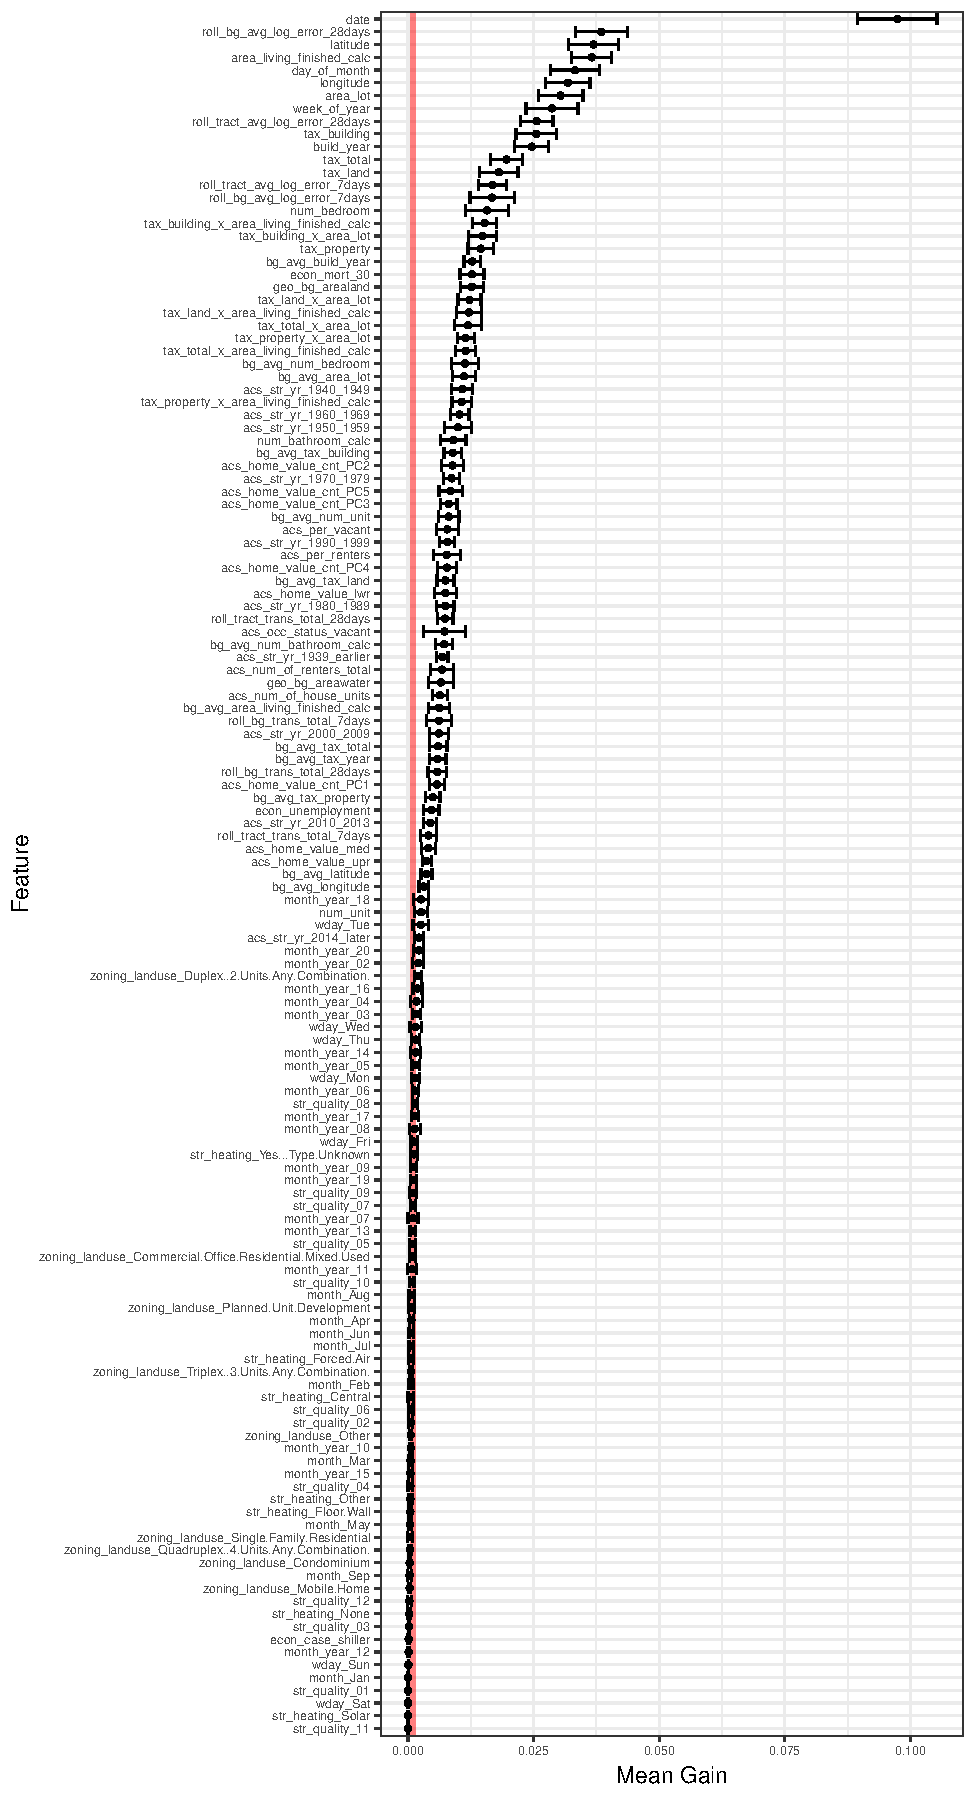
\includegraphics[width=1\linewidth]{zillow-prize_files/figure-latex/feat-importance-1} \caption{Mean Feature Importance Based on Cross Validation Using Basic XGBoost Model}\label{fig:feat-importance}
\end{figure}

To reduce the complexity and computation time our of modeling, we are
going to remove the feature that consistantly did not provide much value
by cutting off the number of features we'll use at a mean gain at
\texttt{0.001} (red line).

\begin{Shaded}
\begin{Highlighting}[]
\NormalTok{features_to_use <-}\StringTok{ }\NormalTok{feature_avg }\OperatorTok\StringTok{ }
\StringTok{  }\KeywordTok{filter}\NormalTok{(mean }\OperatorTok{>=}\StringTok{ }\FloatTok{0.001}\NormalTok{) }\OperatorTok
\StringTok{  }\NormalTok{.}\OperatorTok{$}\NormalTok{Feature}
\end{Highlighting}
\end{Shaded}

\chapter{Modeling}\label{modeling}

For our first pass a submission, we are going to use the XGBoost model.
This model has seen much success in Kaggle competitions and wide use
across industry and academia due to its flexiblity, speed, and range of
modeling tasks it can be applied to. We'll start by creating a base line
model and then try our hand at tuning a few of the XGBoost parameters to
see how of performance changes.

\section{XGBoost}\label{xgboost}

XGBoost, which stands for eXtreme Gradient Boosting, is a highly
optimized and flexible implementation of gradient boosted decision
trees. At a high level boosted trees work by creating ensembles of
decision trees and uses gradient boosting (additive training) to combine
each of the tree's predictions into one strong prediction by optimizing
over any differentiable loss function. In practice a regularization
penalty is added to the loss function to help control complexity.

Decision trees, particularly XGBoost is widely used for several reasons
such as its flexibilty to be used for numerous problem types across both
regression and classification, it's invariance to scaling inputs, and
it's ability to scale to handle large amounts of data.

For more information about XGBoost see Chen \& Guestrin\footnote{XGBoost:
  A Scalable Tree Boosting System \url{https://arxiv.org/abs/1603.02754}}
and Gradient Boosting in general, Fridmean (1999)\footnote{Greedy
  Function Approximation: A Gradient Boosting Machine
  \url{http://statweb.stanford.edu/~jhf/ftp/trebst.pdf}}

\section{Our Recipe for Success}\label{our-recipe-for-success}

As a reminder our recipe for our transformations are stored in
\texttt{rec} that we created in Chapter 4. It's looks like this

\begin{Shaded}
\begin{Highlighting}[]
\NormalTok{rec}
\end{Highlighting}
\end{Shaded}

\begin{verbatim}
## Data Recipe
## 
## Inputs:
## 
##       role #variables
##    outcome          1
##  predictor         98
## 
## Operations:
## 
## Mean Imputation for starts_with("roll_")
## Zero variance filter on all_numeric()
## Box-Cox transformation on 6 items
## Dummy variables from all_nominal()
## Interactions with starts_with("tax_"):starts_with("area_")
## Centering for all_numeric(), -all_outcomes()
## Scaling for all_numeric(), -all_outcomes()
## PCA extraction with starts_with("acs_home_value_cnt")
## Zero variance filter on all_numeric()
\end{verbatim}

\section{Base Line Model}\label{base-line-model}

\begin{quote}
Alice: ``Would you tell me, please, which way I ought to go from here?''

The Cheshire Cat: ``That depends a good deal on where you want to get
to.''

Alice: ``I don't much care where.''

The Cheshire Cat: ``Then it doesn't matter which way you go.''

--- The Adventures of Alice in Wonderland, on the need for base line
models in machine learning (that's my interpretation at least)
\end{quote}

Making Predictive models is an iterative process, a process in which it
is easy to get pulled in wrong directions by needless complexity,
fruitless tweaks, and soul crushingly poor performing ideas you thought
might actually work.

To help tether ourselves to reality, it is useful to generate a base
line model to compare all other models against before we get into any of
the more complex tasks like parameter tuning. This will help guide what
direction we should take next so we don't end up like Alice.

Kaggle competitions have done wonders for our collective obession for
improving predictive accuracy with wild disregard for the time and
effort it took to achieve that improvement. In a typical business or
scientific academic application, improvement in predictive accuracy has
to be balanced with the cost of acheiving it. A base line model can help
use measure these diminishing returns.

For our base line model, we will use the top \texttt{20} features
returned from our feature selection process in an xgboost model with
default parameter settings and with \texttt{nrounds}, the maximum number
of boosting iterations, set to \texttt{1000}

\begin{Shaded}
\begin{Highlighting}[]
\NormalTok{features_to_use_baseline <-}\StringTok{ }\NormalTok{feature_avg }\OperatorTok\StringTok{ }
\StringTok{  }\KeywordTok{arrange}\NormalTok{(}\KeywordTok{desc}\NormalTok{(mean)) }\OperatorTok\StringTok{ }
\StringTok{  }\KeywordTok{head}\NormalTok{(}\DecValTok{20}\NormalTok{) }\OperatorTok\StringTok{ }
\StringTok{  }\NormalTok{.}\OperatorTok{$}\NormalTok{Feature}

\NormalTok{d_prepped <-}\StringTok{ }\KeywordTok{prep}\NormalTok{(rec)}

\NormalTok{train_df <-}\StringTok{ }\KeywordTok{bake}\NormalTok{(d_prepped, }\DataTypeTok{newdata =}\NormalTok{ d)}

\NormalTok{x_train <-}\StringTok{ }\NormalTok{train_df }\OperatorTok\StringTok{ }
\StringTok{  }\KeywordTok{select}\NormalTok{(features_to_use_baseline) }\OperatorTok
\StringTok{  }\KeywordTok{as.matrix}\NormalTok{()}

\NormalTok{y_train <-}\StringTok{ }\NormalTok{train_df}\OperatorTok{$}\NormalTok{log_error}

\NormalTok{xgb_train_data <-}\StringTok{ }\KeywordTok{xgb.DMatrix}\NormalTok{(x_train, }\DataTypeTok{label =}\NormalTok{ y_train)}

\NormalTok{base_model <-}\StringTok{ }\KeywordTok{xgb.train}\NormalTok{(}\DataTypeTok{data =}\NormalTok{ xgb_train_data,}
                        \DataTypeTok{objective =} \StringTok{'reg:linear'}\NormalTok{,}
                        \DataTypeTok{verbose =} \OtherTok{FALSE}\NormalTok{,}
                        \DataTypeTok{nrounds =} \DecValTok{1000}\NormalTok{,}
                        \DataTypeTok{nthread =} \DecValTok{20}\NormalTok{)}
\end{Highlighting}
\end{Shaded}

\subsection{Making Predictions with Base Line
Model}\label{making-predictions-with-base-line-model}

Now we finally get to make our first predictions! Since we'll be doing
this again and potentially many times, let's make a helper function
\texttt{predict\_date()} to do this. This function will take, the
parcels (\texttt{parcel\_id}) and the dates (\texttt{predict\_date}) we
wish to predict, along with the model (\texttt{mdl}) and features we
want to use to (\texttt{features\_to\_use}) to do the predictions

\begin{Shaded}
\begin{Highlighting}[]
\NormalTok{predict_date <-}\StringTok{ }\ControlFlowTok{function}\NormalTok{(parcel_id, predict_date, mdl, features_to_use) \{}

\NormalTok{d_predict_ids <-}\StringTok{ }\NormalTok{properties }\OperatorTok
\StringTok{  }\KeywordTok{filter}\NormalTok{(id_parcel }\OperatorTok\StringTok{ }\NormalTok{parcel_id) }\OperatorTok
\StringTok{  }\KeywordTok{crossing}\NormalTok{(}\DataTypeTok{date =}\NormalTok{ predict_date)}

\NormalTok{d_predict <-}\StringTok{ }\NormalTok{d_predict_ids }\OperatorTok
\StringTok{  }\KeywordTok{mutate}\NormalTok{(}
    \DataTypeTok{year =} \KeywordTok{year}\NormalTok{(date),}
    \DataTypeTok{month_year =} \KeywordTok{make_date}\NormalTok{(}\KeywordTok{year}\NormalTok{(date), }\KeywordTok{month}\NormalTok{(date)),}
    \DataTypeTok{month =} \KeywordTok{month}\NormalTok{(date, }\DataTypeTok{label =} \OtherTok{TRUE}\NormalTok{),}
    \DataTypeTok{week =} \KeywordTok{floor_date}\NormalTok{(date, }\DataTypeTok{unit =} \StringTok{"week"}\NormalTok{),}
    \DataTypeTok{week_of_year =} \KeywordTok{week}\NormalTok{(date),}
    \DataTypeTok{week_since_start =}\NormalTok{ (}\KeywordTok{min}\NormalTok{(date) }\OperatorTok\StringTok{ }\NormalTok{date }\OperatorTok\StringTok{ }\KeywordTok{dweeks}\NormalTok{()) }\OperatorTok{+}\StringTok{ }\DecValTok{1}\NormalTok{,}
    \DataTypeTok{wday =} \KeywordTok{wday}\NormalTok{(date, }\DataTypeTok{label =} \OtherTok{TRUE}\NormalTok{),}
    \DataTypeTok{day_of_month =} \KeywordTok{day}\NormalTok{(date)}
\NormalTok{  ) }\OperatorTok\StringTok{ }
\StringTok{  }\KeywordTok{left_join}\NormalTok{(econ_features, }\DataTypeTok{by =} \StringTok{"date"}\NormalTok{) }\OperatorTok
\StringTok{  }\KeywordTok{left_join}\NormalTok{(roll_bg, }\DataTypeTok{by =} \KeywordTok{c}\NormalTok{(}\StringTok{"id_geo_bg_fips"}\NormalTok{, }\StringTok{"date"}\NormalTok{)) }\OperatorTok
\StringTok{  }\KeywordTok{left_join}\NormalTok{(roll_tract, }\DataTypeTok{by =} \KeywordTok{c}\NormalTok{(}\StringTok{"id_geo_tract_fips"}\NormalTok{, }\StringTok{"date"}\NormalTok{)) }\OperatorTok
\StringTok{  }\KeywordTok{select}\NormalTok{(}
    \OperatorTok{-}\NormalTok{id_parcel,}
    \OperatorTok{-}\NormalTok{week,}
    \OperatorTok{-}\NormalTok{region_city,}
    \OperatorTok{-}\NormalTok{region_zip,}
    \OperatorTok{-}\NormalTok{area_lot_jitter,}
    \OperatorTok{-}\NormalTok{area_lot_quantile,}
    \OperatorTok{-}\NormalTok{lat, }\CommentTok{# we have other lat/lon features}
    \OperatorTok{-}\NormalTok{lon, }
    \OperatorTok{-}\KeywordTok{starts_with}\NormalTok{(}\StringTok{"id_geo"}\NormalTok{)}
\NormalTok{  ) }\OperatorTok
\StringTok{  }\KeywordTok{mutate}\NormalTok{(}
    \DataTypeTok{date =} \KeywordTok{as.numeric}\NormalTok{(date),}
    \DataTypeTok{year =} \KeywordTok{factor}\NormalTok{(year, }\DataTypeTok{levels =} \KeywordTok{sort}\NormalTok{(}\KeywordTok{unique}\NormalTok{(year)), }\DataTypeTok{ordered =} \OtherTok{TRUE}\NormalTok{),}
    \DataTypeTok{month_year =} \KeywordTok{factor}\NormalTok{(}
      \KeywordTok{as.character}\NormalTok{(month_year), }
      \DataTypeTok{levels =} \KeywordTok{as.character}\NormalTok{(}\KeywordTok{unique}\NormalTok{(}\KeywordTok{sort}\NormalTok{(month_year))), }
      \DataTypeTok{ordered =} \OtherTok{TRUE}\NormalTok{),}
    \DataTypeTok{str_quality =} \KeywordTok{factor}\NormalTok{(str_quality, }\DataTypeTok{levels =} \DecValTok{12}\OperatorTok{:}\DecValTok{1}\NormalTok{, }\DataTypeTok{ordered =} \OtherTok{TRUE}\NormalTok{)}
\NormalTok{  )}

\NormalTok{eval_df <-}\StringTok{ }\KeywordTok{bake}\NormalTok{(d_prepped, }\DataTypeTok{newdata =}\NormalTok{ d_predict)}

\NormalTok{x_eval <-}\StringTok{ }\NormalTok{eval_df }\OperatorTok\StringTok{ }
\StringTok{  }\KeywordTok{select}\NormalTok{(features_to_use) }\OperatorTok\StringTok{ }
\StringTok{  }\KeywordTok{as.matrix}\NormalTok{()}

\NormalTok{preds <-}\StringTok{ }\KeywordTok{predict}\NormalTok{(mdl, x_eval)}

\NormalTok{properties_predict <-}\StringTok{ }\NormalTok{d_predict_ids }\OperatorTok
\StringTok{  }\KeywordTok{select}\NormalTok{(}
\NormalTok{    id_parcel,}
\NormalTok{    date}
\NormalTok{  ) }\OperatorTok
\StringTok{  }\KeywordTok{mutate}\NormalTok{(}
    \DataTypeTok{pred =}\NormalTok{ preds}
\NormalTok{    ) }\OperatorTok
\StringTok{  }\KeywordTok{spread}\NormalTok{(date, pred)}

\KeywordTok{names}\NormalTok{(properties_predict) <-}\StringTok{ }\KeywordTok{c}\NormalTok{(}\StringTok{"ParcelId"}\NormalTok{, }\StringTok{"201610"}\NormalTok{, }\StringTok{"201611"}\NormalTok{, }
                               \StringTok{"201612"}\NormalTok{, }\StringTok{"201710"}\NormalTok{, }\StringTok{"201711"}\NormalTok{, }\StringTok{"201712"}\NormalTok{)}

\NormalTok{properties_predict}

\NormalTok{\}}
\end{Highlighting}
\end{Shaded}

The submission requires a prediction for Oct-Dec 2016 and Oct-Dec 2017.
This means that the prediction is for any day in that month. For our
example submissions, we are going to set the date to the first Wednesday
in each month. This is completely arbitrary, but provides a simple
starting point. Another approach would be to make predictions for every
day in each month and submit the mean prediction for each month. We'll
save this for later work.

\begin{Shaded}
\begin{Highlighting}[]
\CommentTok{# first wednesday in each month}
\NormalTok{predict_dates <-}\StringTok{ }\KeywordTok{date}\NormalTok{(}\KeywordTok{c}\NormalTok{(}\StringTok{"2016-10-06"}\NormalTok{, }\StringTok{"2016-11-02"}\NormalTok{, }\StringTok{"2016-12-07"}\NormalTok{, }
                        \StringTok{"2017-10-04"}\NormalTok{, }\StringTok{"2017-11-01"}\NormalTok{, }\StringTok{"2017-12-06"}\NormalTok{))}

\CommentTok{# split parcels to chunck our predictions}
\NormalTok{id_parcels <-}\StringTok{ }\NormalTok{properties}\OperatorTok{$}\NormalTok{id_parcel}
\NormalTok{id_parcel_splits <-}\StringTok{ }\KeywordTok{split}\NormalTok{(id_parcels, }\KeywordTok{ceiling}\NormalTok{(}\KeywordTok{seq_along}\NormalTok{(id_parcels) }\OperatorTok{/}\StringTok{ }\DecValTok{5000}\NormalTok{))}
\end{Highlighting}
\end{Shaded}

Now make the predictions with \texttt{base\_model}

\begin{Shaded}
\begin{Highlighting}[]
\NormalTok{base_predict_list <-}\StringTok{ }\KeywordTok{lapply}\NormalTok{(id_parcel_splits, }\ControlFlowTok{function}\NormalTok{(i) \{}
  
\NormalTok{  pred_df <-}\StringTok{ }\KeywordTok{predict_date}\NormalTok{(}
    \DataTypeTok{parcel_id =}\NormalTok{ i, }
    \DataTypeTok{predict_date =}\NormalTok{ predict_dates, }
    \DataTypeTok{mdl =}\NormalTok{ base_model,}
    \DataTypeTok{features_to_use =}\NormalTok{ features_to_use_baseline}
\NormalTok{    )}
\NormalTok{  \})}

\CommentTok{# they only evaluate to 4 decimcals so round to save space}
\CommentTok{# Convert ParcelId to integer to prevent Sci Notation that causes}
\CommentTok{# issues with submission}
\NormalTok{base_predict_df <-}\StringTok{ }\KeywordTok{bind_rows}\NormalTok{(base_predict_list) }\OperatorTok
\StringTok{  }\KeywordTok{mutate_at}\NormalTok{(}\KeywordTok{vars}\NormalTok{(}\StringTok{`}\DataTypeTok{201610}\StringTok{`}\OperatorTok{:}\StringTok{`}\DataTypeTok{201712}\StringTok{`}\NormalTok{), round, }\DataTypeTok{digits =} \DecValTok{4}\NormalTok{) }\OperatorTok
\StringTok{  }\KeywordTok{mutate}\NormalTok{(}\DataTypeTok{ParcelId =} \KeywordTok{as.integer}\NormalTok{(ParcelId)) }\OperatorTok
\StringTok{  }\KeywordTok{as.data.frame}\NormalTok{()}

\KeywordTok{write_csv}\NormalTok{(base_predict_df, }\StringTok{"submissions/base_submit.csv"}\NormalTok{)}
\end{Highlighting}
\end{Shaded}

The resulting MAE of this submission was \texttt{0.0789722} on the
public leaderboard. Not that great, but hey at least we have room to
improve.

Save this value for comparison

\begin{Shaded}
\begin{Highlighting}[]
\NormalTok{base_mae <-}\StringTok{ }\FloatTok{0.0789722}
\end{Highlighting}
\end{Shaded}

Let's see if tuning the parameters of the XGBoost model can help improve
that.

\section{Hyperparameter Optimization}\label{hyperparameter-optimization}

The double edged sword of the XGBoost model is how widely varying the
predictions it generates can be depending on what the models
hyperparameters are set to. The good is that it allows us to be very
flexible across many different datasets, the bad is it almost always
requires us to perform some type of hyperparameter optimization to fine
tune its' performance. The ugly is the code needed to perform this.

Our parameter optimization strategy is as follows

\begin{enumerate}
\def\labelenumi{\arabic{enumi}.}
\item
  Create a scoring function to capture model performance using MAE
\item
  Use 5-fold cross validation to resample our training data
\item
  Randomly generate intital parameter combinations.
\item
  Using step 3 as an intital input, use a surrogate Random Forest model
  to progressively zoom into parameter space based on the average
  performance of parameter sets across the resampled data on our scoring
  function. We will set this to 4 runs for now, zooming further down
  each time.
\end{enumerate}

\subsection{Creating Our Scoring
Function}\label{creating-our-scoring-function}

To assess our parameter tuning performance we will create the function
\texttt{xgboost\_regress\_score()} that will capture the MAE of each
resample and parameter combination of our data

\begin{Shaded}
\begin{Highlighting}[]
\CommentTok{# create scoring function -------------------------------------------------}

\NormalTok{xgboost_regress_score <-}\StringTok{ }\ControlFlowTok{function}\NormalTok{(train_df, target_var, params, eval_df, ...) \{}
    
\NormalTok{    X_train <-}\StringTok{ }\NormalTok{train_df }\OperatorTok\StringTok{ }
\StringTok{      }\KeywordTok{select}\NormalTok{(features_to_use) }\OperatorTok
\StringTok{      }\KeywordTok{as.matrix}\NormalTok{()}
    
\NormalTok{    y_train <-}\StringTok{ }\NormalTok{train_df[[target_var]]}
\NormalTok{    xgb_train_data <-}\StringTok{ }\KeywordTok{xgb.DMatrix}\NormalTok{(X_train, }\DataTypeTok{label =}\NormalTok{ y_train)}
    
\NormalTok{    X_eval <-}\StringTok{ }\NormalTok{eval_df }\OperatorTok\StringTok{ }
\StringTok{      }\KeywordTok{select}\NormalTok{(features_to_use) }\OperatorTok\StringTok{ }
\StringTok{      }\KeywordTok{as.matrix}\NormalTok{()}
    
\NormalTok{    y_eval <-}\StringTok{ }\NormalTok{eval_df[[target_var]]}
    
\NormalTok{    xgb_eval_data <-}\StringTok{ }\KeywordTok{xgb.DMatrix}\NormalTok{(X_eval, }\DataTypeTok{label =}\NormalTok{ y_eval)}
    
\NormalTok{    model <-}\StringTok{ }\KeywordTok{xgb.train}\NormalTok{(}\DataTypeTok{params =}\NormalTok{ params,}
                       \DataTypeTok{data =}\NormalTok{ xgb_train_data,}
                       \DataTypeTok{watchlist =} \KeywordTok{list}\NormalTok{(}\DataTypeTok{train =}\NormalTok{ xgb_train_data, }\DataTypeTok{eval =}\NormalTok{ xgb_eval_data),}
                       \DataTypeTok{objective =} \StringTok{'reg:linear'}\NormalTok{,}
                       \DataTypeTok{verbose =} \OtherTok{FALSE}\NormalTok{,}
                       \DataTypeTok{nthread =} \DecValTok{20}\NormalTok{,}
\NormalTok{                       ...)}
    
\NormalTok{    preds <-}\StringTok{ }\KeywordTok{predict}\NormalTok{(model, xgb_eval_data)}
    
    \KeywordTok{list}\NormalTok{(}\DataTypeTok{mae =} \KeywordTok{MAE}\NormalTok{(preds, y_eval))}
    
\NormalTok{  \}}
\end{Highlighting}
\end{Shaded}

\subsection{Parameter Search Space}\label{parameter-search-space}

We will use the following parameters

\begin{itemize}
\tightlist
\item
  \texttt{eta} {[}default=0.3, alias: \texttt{learning\_rate}{]}

  \begin{itemize}
  \tightlist
  \item
    Step size shrinkage used in update to prevents overfitting. After
    each boosting step, we can directly get the weights of new features,
    and eta shrinks the feature weights to make the boosting process
    more conservative.
  \item
    range: {[}0, 1{]}
  \end{itemize}
\item
  \texttt{gamma} {[}default=0, alias: \texttt{min\_split\_loss}{]}

  \begin{itemize}
  \tightlist
  \item
    Minimum loss reduction required to make a further partition on a
    leaf node of the tree. The larger \texttt{gamma} is, the more
    conservative the algorithm will be.
  \item
    range{[}0, \texttt{Inf}{]}
  \end{itemize}
\item
  \texttt{max\_depth} {[}default=6{]}

  \begin{itemize}
  \tightlist
  \item
    Maximum depth of a tree. Increasing this value will make the model
    more complex and more likely to overfit. 0 indicates no limit.
  \item
    range: {[}0, \texttt{Inf}{]}
  \end{itemize}
\item
  \texttt{min\_child\_weight} {[}default=1{]}

  \begin{itemize}
  \tightlist
  \item
    Minimum sum of instance weight (hessian) needed in a child. If the
    tree partition step results in a leaf node with the sum of instance
    weight less than \texttt{min\_child\_weight}, then the building
    process will give up further partitioning. In linear regression
    task, this simply corresponds to minimum number of instances needed
    to be in each node. The larger \texttt{min\_child\_weight} is, the
    more conservative the algorithm will be.
  \item
    range: {[}0, \texttt{Inf}{]}
  \end{itemize}
\item
  \texttt{subsample} {[}default=1{]}

  \begin{itemize}
  \tightlist
  \item
    Subsample ratio of the training instances. Setting it to 0.5 means
    that XGBoost would randomly sample half of the training data prior
    to growing trees. and this will prevent overfitting. Subsampling
    will occur once in every boosting iteration.
  \item
    range: (0, 1{]}
  \end{itemize}
\item
  \texttt{colsample\_bytree} {[}default=1{]}

  \begin{itemize}
  \tightlist
  \item
    Subsample ratio of columns when constructing each tree. Subsampling
    will occur once in every boosting iteration.
  \item
    range: (0, 1{]}
  \end{itemize}
\end{itemize}

Based on the performance of these optimizations other parameters could
be included later. I set the ranges on these parameters with the idea
that our base line model might be overfiting.

\begin{Shaded}
\begin{Highlighting}[]
\KeywordTok{library}\NormalTok{(ParamHelpers)}
\CommentTok{# make parameter set ------------------------------------------------------}
\NormalTok{xgboost_random_params <-}
\StringTok{  }\KeywordTok{makeParamSet}\NormalTok{(}
    \KeywordTok{makeIntegerParam}\NormalTok{(}\StringTok{'max_depth'}\NormalTok{, }\DataTypeTok{lower =} \DecValTok{1}\NormalTok{, }\DataTypeTok{upper =} \DecValTok{15}\NormalTok{),}
    \KeywordTok{makeNumericParam}\NormalTok{(}\StringTok{'eta'}\NormalTok{, }\DataTypeTok{lower =} \FloatTok{0.01}\NormalTok{, }\DataTypeTok{upper =} \FloatTok{0.1}\NormalTok{),}
    \KeywordTok{makeNumericParam}\NormalTok{(}\StringTok{'gamma'}\NormalTok{, }\DataTypeTok{lower =} \DecValTok{0}\NormalTok{, }\DataTypeTok{upper =} \DecValTok{5}\NormalTok{),}
    \KeywordTok{makeIntegerParam}\NormalTok{(}\StringTok{'min_child_weight'}\NormalTok{, }\DataTypeTok{lower =} \DecValTok{1}\NormalTok{, }\DataTypeTok{upper =} \DecValTok{100}\NormalTok{),}
    \KeywordTok{makeNumericParam}\NormalTok{(}\StringTok{'subsample'}\NormalTok{, }\DataTypeTok{lower =} \FloatTok{0.25}\NormalTok{, }\DataTypeTok{upper =} \FloatTok{0.9}\NormalTok{),}
    \KeywordTok{makeNumericParam}\NormalTok{(}\StringTok{'colsample_bytree'}\NormalTok{, }\DataTypeTok{lower =} \FloatTok{0.25}\NormalTok{, }\DataTypeTok{upper =} \FloatTok{0.9}\NormalTok{)}
\NormalTok{  )}
\end{Highlighting}
\end{Shaded}

\subsection{5-fold Cross Validation}\label{fold-cross-validation}

Set up our resampling via 5 fold cross validation

\begin{Shaded}
\begin{Highlighting}[]
\CommentTok{# create cv resampling ----------------------------------------------------}
\NormalTok{resamples <-}\StringTok{ }\KeywordTok{vfold_cv}\NormalTok{(d, }\DataTypeTok{v =} \DecValTok{5}\NormalTok{) }
\end{Highlighting}
\end{Shaded}

\subsection{Random Forest Search of Parameter
Space}\label{random-forest-search-of-parameter-space}

All of the heavy lifting for the surrogate Random Forest model is
contained in the \texttt{tidytune::surrogate\_search()} function.

The progressive zoom into more promising parameter space is done by
passing a vector to \texttt{n} and \texttt{n\_canidates}. Higher values
for \texttt{n\_candidates} will restrict the search to better performing
areas and lower values increase the randnomness (with \texttt{0} falling
back on random search).\texttt{n} is the number of runs of the surrogate
model that will run for each of our 5 folds.

\texttt{top\_n} is set to 5, which tells the model out of the top
\texttt{n\_candidates} pass along the \texttt{top\_n} to the next round.

We will do for runs of the surrogate Random Forest model, zooming into
more performant parameter space each time.

\begin{Shaded}
\begin{Highlighting}[]
\KeywordTok{library}\NormalTok{(MLmetrics)}
\KeywordTok{library}\NormalTok{(xgboost)}
\KeywordTok{library}\NormalTok{(tidytune)}

\CommentTok{# perform surrogate search over parameters --------------------------------}
\NormalTok{n <-}\StringTok{ }\KeywordTok{c}\NormalTok{(}\DecValTok{10}\NormalTok{, }\DecValTok{5}\NormalTok{, }\DecValTok{3}\NormalTok{, }\DecValTok{2}\NormalTok{)}
\CommentTok{# start with random and then zoom in}
\NormalTok{n_candidates <-}\StringTok{ }\KeywordTok{c}\NormalTok{(}\DecValTok{0}\NormalTok{, }\DecValTok{10}\NormalTok{, }\DecValTok{100}\NormalTok{, }\DecValTok{1000}\NormalTok{)}

\NormalTok{search_results <-}\StringTok{ }
\StringTok{  }\KeywordTok{surrogate_search}\NormalTok{(}
    \DataTypeTok{resamples =}\NormalTok{ resamples,}
    \DataTypeTok{recipe =}\NormalTok{ rec,}
    \DataTypeTok{param_set =}\NormalTok{ xgboost_random_params,}
    \DataTypeTok{n =}\NormalTok{ n,}
    \DataTypeTok{scoring_func =}\NormalTok{ xgboost_regress_score,}
    \DataTypeTok{nrounds =} \DecValTok{1000}\NormalTok{,}
    \DataTypeTok{early_stopping_rounds =} \DecValTok{20}\NormalTok{,}
    \DataTypeTok{eval_metric =} \StringTok{'mae'}\NormalTok{,}
    \DataTypeTok{input =} \OtherTok{NULL}\NormalTok{,}
    \DataTypeTok{surrogate_target =} \StringTok{'mae'}\NormalTok{,}
    \DataTypeTok{n_candidates =}\NormalTok{ n_candidates,}
    \DataTypeTok{top_n =} \DecValTok{5}
\NormalTok{  )}
\end{Highlighting}
\end{Shaded}

\begin{Shaded}
\begin{Highlighting}[]
\NormalTok{search_summary <-}\StringTok{ }
\StringTok{  }\NormalTok{search_results }\OperatorTok
\StringTok{  }\KeywordTok{group_by_at}\NormalTok{(}\KeywordTok{getParamIds}\NormalTok{(xgboost_random_params)) }\OperatorTok
\StringTok{  }\KeywordTok{summarise}\NormalTok{(}\DataTypeTok{mae =} \KeywordTok{mean}\NormalTok{(mae)) }\OperatorTok
\StringTok{  }\KeywordTok{arrange}\NormalTok{(mae)}
\end{Highlighting}
\end{Shaded}

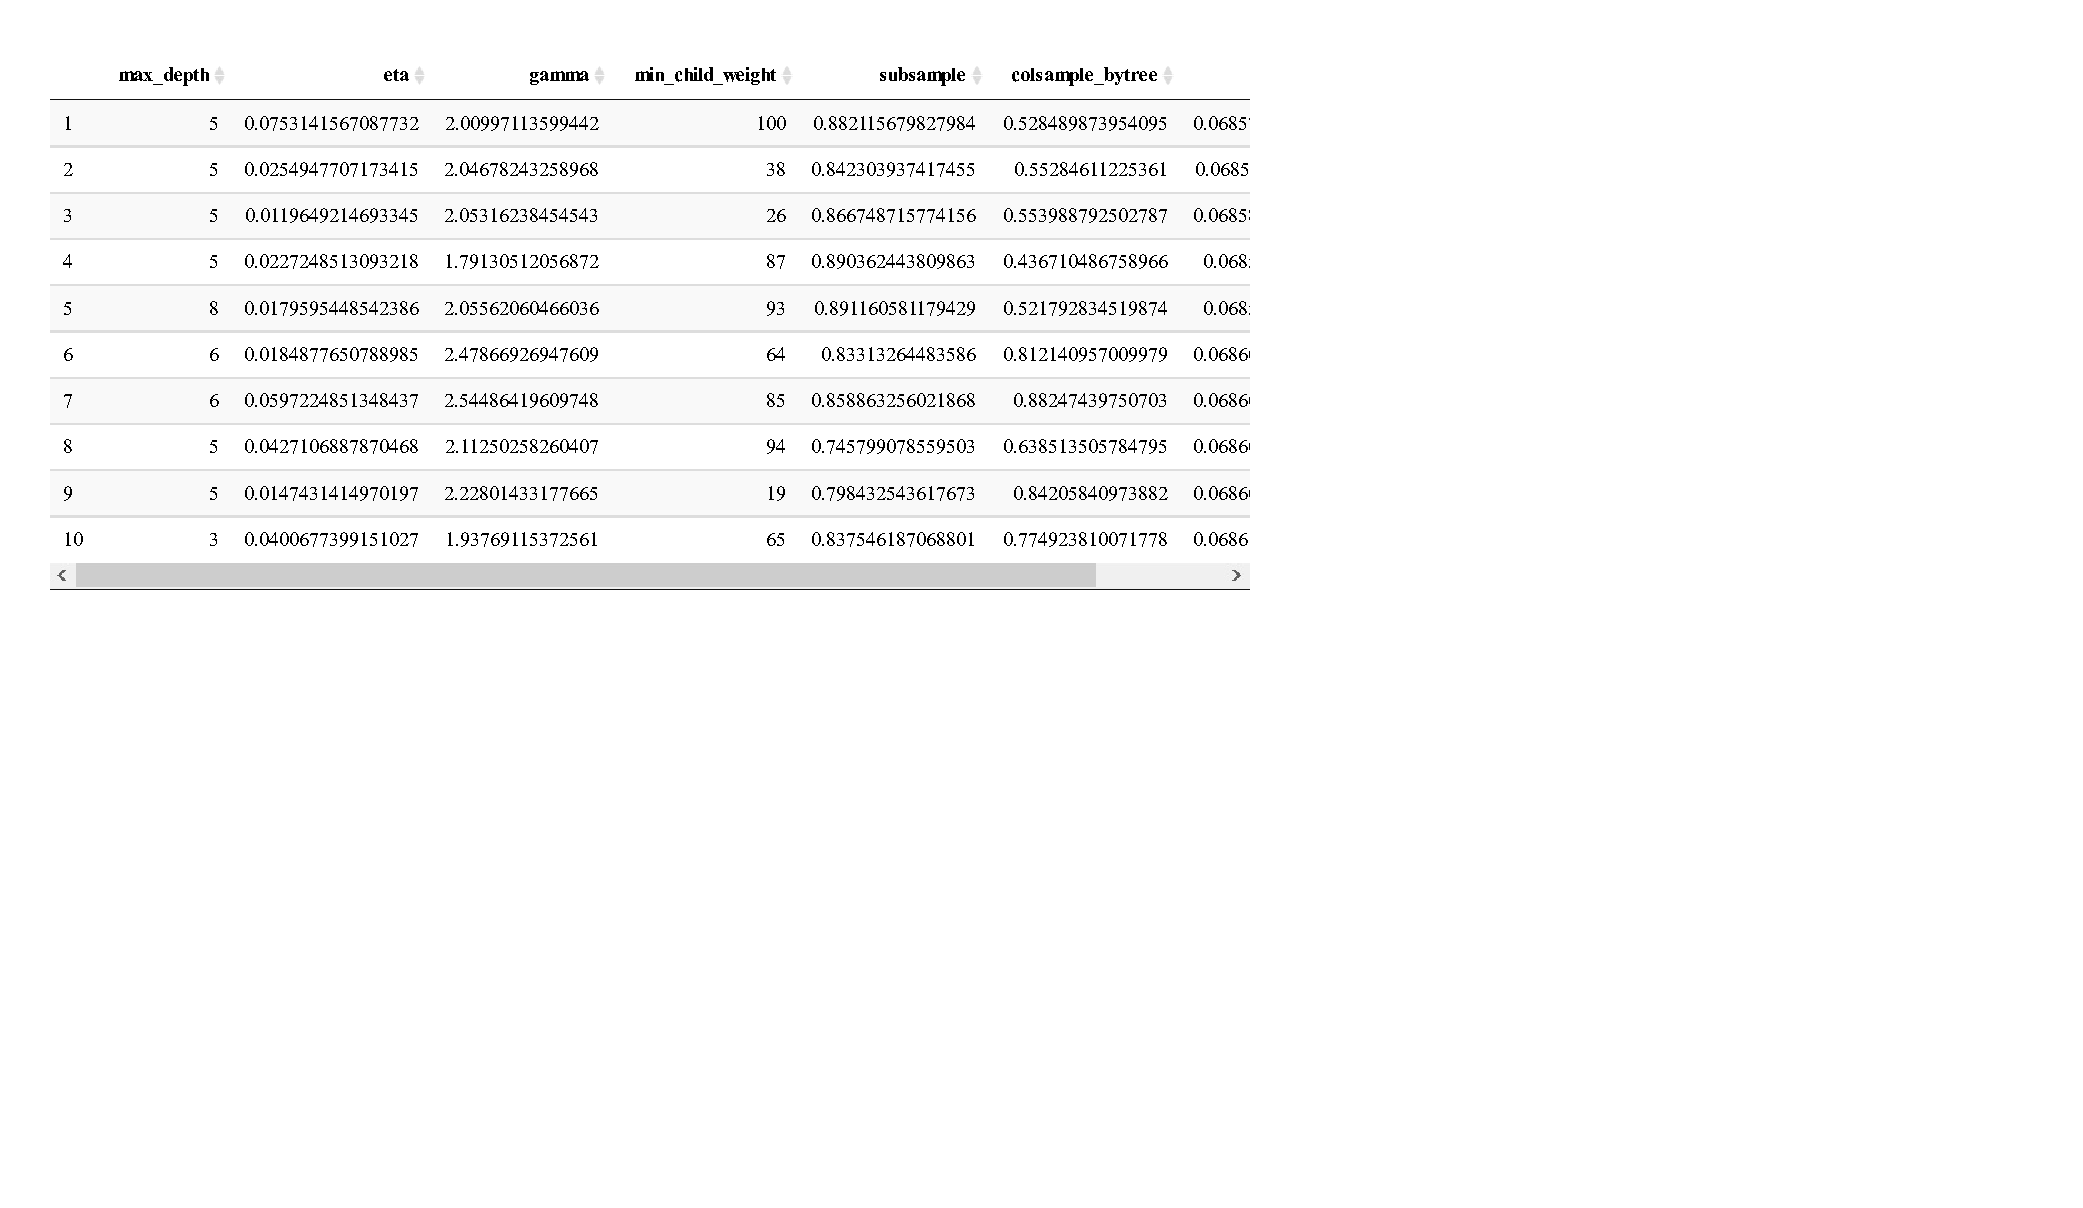
\includegraphics{zillow-prize_files/figure-latex/unnamed-chunk-16-1.pdf}

\subsection{Exploring Parameter Space}\label{exploring-parameter-space}

Let's explore the parameter space some, shall we?

\begin{Shaded}
\begin{Highlighting}[]
\NormalTok{search_results }\OperatorTok
\StringTok{   }\KeywordTok{group_by_at}\NormalTok{(}
     \KeywordTok{c}\NormalTok{(}\StringTok{"surrogate_run"}\NormalTok{, }
       \StringTok{"surrogate_iteration"}\NormalTok{,}
       \StringTok{"param_id"}\NormalTok{,}
      \KeywordTok{getParamIds}\NormalTok{(xgboost_random_params)}
\NormalTok{       )}
\NormalTok{     ) }\OperatorTok
\StringTok{   }\KeywordTok{summarise}\NormalTok{(}\DataTypeTok{mae =} \KeywordTok{mean}\NormalTok{(mae)) }\OperatorTok
\StringTok{   }\KeywordTok{ungroup}\NormalTok{() }\OperatorTok
\StringTok{  }\KeywordTok{mutate}\NormalTok{(}\DataTypeTok{surrogate_run =} \KeywordTok{factor}\NormalTok{(surrogate_run)) }\OperatorTok
\KeywordTok{ggplot}\NormalTok{(}\KeywordTok{aes}\NormalTok{(}\DataTypeTok{x =}\NormalTok{ subsample, }\DataTypeTok{y =}\NormalTok{ gamma, }\DataTypeTok{size =}\NormalTok{ mae)) }\OperatorTok{+}
\StringTok{  }\KeywordTok{geom_point}\NormalTok{(}\KeywordTok{aes}\NormalTok{(}\DataTypeTok{col =}\NormalTok{ surrogate_run)) }\OperatorTok{+}\StringTok{ }
\StringTok{  }\KeywordTok{theme_bw}\NormalTok{() }\OperatorTok{+}\StringTok{ }
\StringTok{  }\KeywordTok{labs}\NormalTok{(}
    \DataTypeTok{y =} \StringTok{"gamma"}\NormalTok{,}
    \DataTypeTok{x =} \StringTok{"subsample"}\NormalTok{,}
    \DataTypeTok{col =} \StringTok{"Surrogate Run"}\NormalTok{,}
    \DataTypeTok{size =} \StringTok{"Average MAE"}
\NormalTok{  )}
\end{Highlighting}
\end{Shaded}

\begin{figure}
\centering
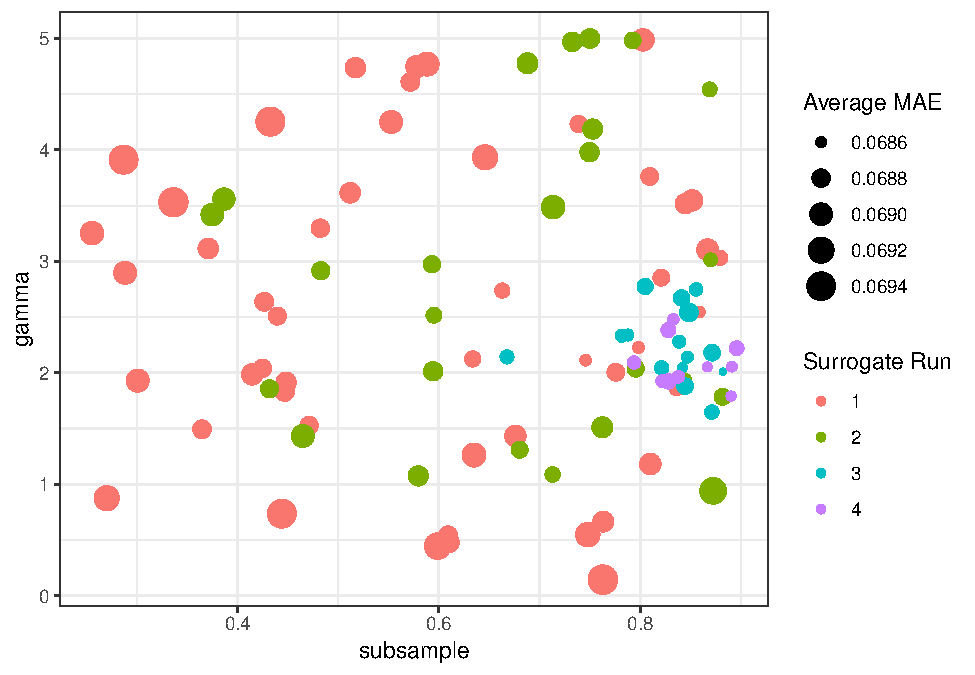
\includegraphics{zillow-prize_files/figure-latex/fig-param-compare-1.pdf}
\caption{\label{fig:fig-param-compare}Gamma and subsample parameters
converging with each surrogate run}
\end{figure}

How does performance increase with each iteration?

\begin{Shaded}
\begin{Highlighting}[]
\NormalTok{search_results }\OperatorTok
\StringTok{  }\KeywordTok{group_by_at}\NormalTok{(}
    \KeywordTok{c}\NormalTok{(}\StringTok{"surrogate_run"}\NormalTok{, }
      \StringTok{"surrogate_iteration"}\NormalTok{,}
      \StringTok{"param_id"}\NormalTok{,}
       \KeywordTok{getParamIds}\NormalTok{(xgboost_random_params)}
\NormalTok{      )}
\NormalTok{    ) }\OperatorTok
\StringTok{  }\KeywordTok{summarise}\NormalTok{(}\DataTypeTok{mae =} \KeywordTok{mean}\NormalTok{(mae)) }\OperatorTok
\StringTok{  }\KeywordTok{ungroup}\NormalTok{() }\OperatorTok
\StringTok{  }\KeywordTok{mutate}\NormalTok{(}\DataTypeTok{surrogate_run =} \KeywordTok{factor}\NormalTok{(surrogate_run)) }\OperatorTok
\StringTok{  }\KeywordTok{arrange}\NormalTok{(}
\NormalTok{    surrogate_run,}
\NormalTok{    surrogate_iteration}
\NormalTok{  ) }\OperatorTok
\StringTok{  }\KeywordTok{mutate}\NormalTok{(}
    \DataTypeTok{iteration =} \KeywordTok{row_number}\NormalTok{()}
\NormalTok{  ) }\OperatorTok
\KeywordTok{ggplot}\NormalTok{(}\KeywordTok{aes}\NormalTok{(}\DataTypeTok{x =}\NormalTok{ iteration, }\DataTypeTok{y =}\NormalTok{ mae)) }\OperatorTok{+}
\StringTok{    }\KeywordTok{geom_smooth}\NormalTok{(}\DataTypeTok{alpha =} \FloatTok{0.2}\NormalTok{, }\DataTypeTok{size =} \FloatTok{0.8}\NormalTok{, }\DataTypeTok{colour =} \StringTok{"grey"}\NormalTok{) }\OperatorTok{+}
\StringTok{  }\KeywordTok{geom_point}\NormalTok{(}\KeywordTok{aes}\NormalTok{(}\DataTypeTok{col =}\NormalTok{ surrogate_run)) }\OperatorTok{+}\StringTok{ }
\StringTok{  }\KeywordTok{theme_bw}\NormalTok{() }\OperatorTok{+}\StringTok{ }
\StringTok{  }\KeywordTok{labs}\NormalTok{(}
    \DataTypeTok{y =} \StringTok{"MAE"}\NormalTok{,}
    \DataTypeTok{x =} \StringTok{"iteration"}\NormalTok{,}
    \DataTypeTok{col =} \StringTok{"Surrogate Run"}
\NormalTok{  )}
\end{Highlighting}
\end{Shaded}

\begin{figure}
\centering
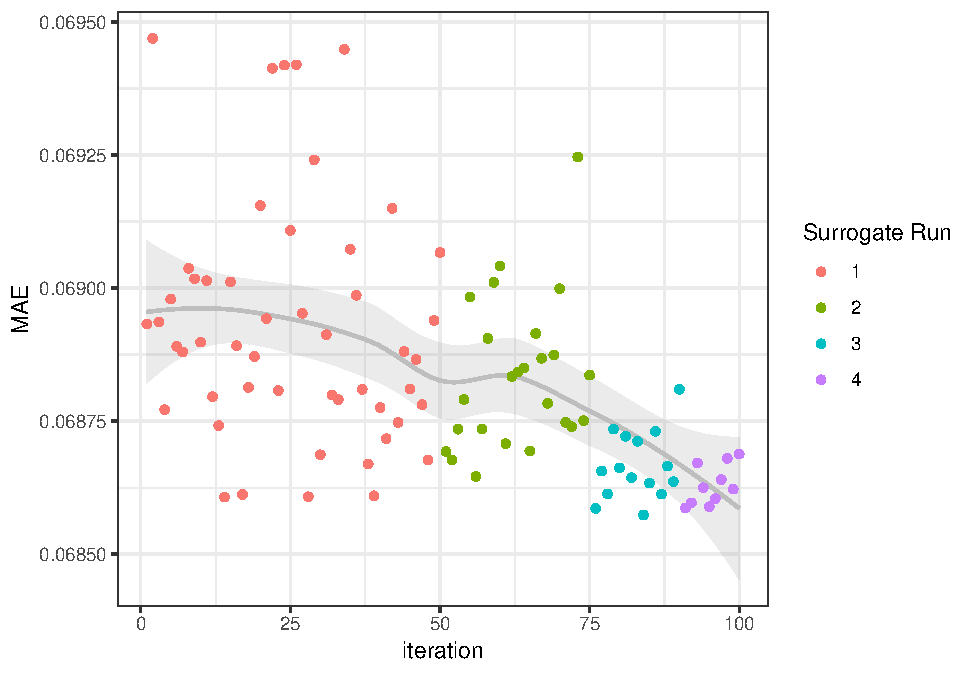
\includegraphics{zillow-prize_files/figure-latex/fig-mae-by-run-1.pdf}
\caption{\label{fig:fig-mae-by-run}Mean Absolute Error Progressively
Decreasing with Each Surrogate Run}
\end{figure}

\section{Tuned Model}\label{tuned-model}

Get the parameter set with the lowest average \texttt{mae} across all
folds

\begin{Shaded}
\begin{Highlighting}[]
\NormalTok{tuned_params <-}\StringTok{ }\NormalTok{search_summary }\OperatorTok
\StringTok{  }\KeywordTok{ungroup}\NormalTok{() }\OperatorTok
\StringTok{  }\KeywordTok{filter}\NormalTok{(mae }\OperatorTok{==}\StringTok{ }\KeywordTok{min}\NormalTok{(mae)) }\OperatorTok
\StringTok{  }\KeywordTok{select}\NormalTok{(}\KeywordTok{getParamIds}\NormalTok{(xgboost_random_params)) }\OperatorTok
\StringTok{  }\KeywordTok{as.list}\NormalTok{()}

\NormalTok{tuned_params}
\end{Highlighting}
\end{Shaded}

\begin{verbatim}
## $max_depth
## [1] 5
## 
## $eta
## [1] 0.07531416
## 
## $gamma
## [1] 2.009971
## 
## $min_child_weight
## [1] 100
## 
## $subsample
## [1] 0.8821157
## 
## $colsample_bytree
## [1] 0.5284899
\end{verbatim}

Since we didn't save the actual models produced in our search, train a
model with the tuned parameters

\begin{Shaded}
\begin{Highlighting}[]
\NormalTok{d_prepped <-}\StringTok{ }\KeywordTok{prep}\NormalTok{(rec)}

\NormalTok{train_df <-}\StringTok{ }\KeywordTok{bake}\NormalTok{(d_prepped, }\DataTypeTok{newdata =}\NormalTok{ d)}

\NormalTok{x_train <-}\StringTok{ }\NormalTok{train_df }\OperatorTok\StringTok{ }
\StringTok{  }\KeywordTok{select}\NormalTok{(features_to_use) }\OperatorTok
\StringTok{  }\KeywordTok{as.matrix}\NormalTok{()}

\NormalTok{y_train <-}\StringTok{ }\NormalTok{train_df}\OperatorTok{$}\NormalTok{log_error}

\NormalTok{xgb_train_data <-}\StringTok{ }\KeywordTok{xgb.DMatrix}\NormalTok{(x_train, }\DataTypeTok{label =}\NormalTok{ y_train)}

\NormalTok{tuned_model <-}\StringTok{ }\KeywordTok{xgb.train}\NormalTok{(}\DataTypeTok{params =}\NormalTok{ tuned_params,}
                         \DataTypeTok{data =}\NormalTok{ xgb_train_data,}
                         \DataTypeTok{objective =} \StringTok{'reg:linear'}\NormalTok{,}
                         \DataTypeTok{verbose =} \OtherTok{FALSE}\NormalTok{,}
                         \DataTypeTok{nthread =} \DecValTok{20}\NormalTok{,}
                         \DataTypeTok{nrounds =} \DecValTok{1000}\NormalTok{)}
\end{Highlighting}
\end{Shaded}

\subsection{Making Predictions with Tuned
Model}\label{making-predictions-with-tuned-model}

Since we already created our helper function \texttt{predict\_dates()}
we can apply it here with our new model

\begin{Shaded}
\begin{Highlighting}[]
\NormalTok{predict_list <-}\StringTok{ }\KeywordTok{lapply}\NormalTok{(id_parcel_splits, }\ControlFlowTok{function}\NormalTok{(i) \{}
  
\NormalTok{  pred_df <-}\StringTok{ }\KeywordTok{predict_date}\NormalTok{(}
    \DataTypeTok{parcel_id =}\NormalTok{ i, }
    \DataTypeTok{predict_date =}\NormalTok{ predict_dates, }
    \DataTypeTok{mdl =}\NormalTok{ tuned_model,}
    \DataTypeTok{features_to_use =}\NormalTok{ features_to_use}
\NormalTok{    )}
\NormalTok{  \})}


\NormalTok{predict_df <-}\StringTok{ }\KeywordTok{bind_rows}\NormalTok{(predict_list) }\OperatorTok
\StringTok{  }\KeywordTok{mutate_at}\NormalTok{(}\KeywordTok{vars}\NormalTok{(}\StringTok{`}\DataTypeTok{201610}\StringTok{`}\OperatorTok{:}\StringTok{`}\DataTypeTok{201712}\StringTok{`}\NormalTok{), round, }\DataTypeTok{digits =} \DecValTok{4}\NormalTok{) }\OperatorTok
\StringTok{  }\KeywordTok{mutate}\NormalTok{(}\DataTypeTok{ParcelId =} \KeywordTok{as.integer}\NormalTok{(ParcelId)) }\OperatorTok
\StringTok{  }\KeywordTok{as.data.frame}\NormalTok{()}

\KeywordTok{write_csv}\NormalTok{(predict_df, }\StringTok{"submissions/submit01.csv"}\NormalTok{)}
\end{Highlighting}
\end{Shaded}

\section{Model Comparison}\label{model-comparison}

This model produced a MAE of \texttt{0.0651839} on the public
leaderboard.

\begin{Shaded}
\begin{Highlighting}[]
\NormalTok{tuned_mae <-}\StringTok{ }\FloatTok{0.0651839}

\CommentTok{# how much did we improve?}
\NormalTok{(tuned_mae }\OperatorTok{-}\StringTok{ }\NormalTok{base_mae) }\OperatorTok{/}\StringTok{ }\NormalTok{base_mae}
\end{Highlighting}
\end{Shaded}

\begin{verbatim}
## [1] -0.1745969
\end{verbatim}

Hey not bad! Our hyperparameter optimization process resulted in a
17.5\% reduction in Mean Abosolute Error when compared to our base line
model. While our absolute position on the leaderboard still isn't very
high, it's a solid first submission that we can build upon and test new
models against. With the top 10 finsishers on the public leaderboard all
averaging 184 submissions each (highest being 449!) this empahsizes the
iterative nature of predictive modeling. We aren't in
1\textsuperscript{st} place with our first submission but we didn't
expect to be.

At this point if we were competing the actual competition we would go
back to the drawing board in start investigating what we could do
differently to improve our score. In our specific case, things like not
making the predicion date the first Wednesday of each month and looking
at the average prediction across all days in the month would be the
first thing I would check to se what kind of improvement resulted. Also
based on @\ref(fig:fig-mae-by-run) it looks like can could further
shrink our parameter space to find more optimal hyperparameter
combinations.

Other things like adding more interaction features or stacking our
xgboost predictions as part of an ensemble of other models is an area to
explore as well.

\chapter{Summary}\label{summary}

Overall we went from basic preprocessing and exploratory analysis, to
feature engineering, to complex parameter tuning. We found out alot
about the data and alot about the modeling process in general.

Using a base line XGBoost model with a limited number of features, we
were able to achieve a MAE of \texttt{0.0789722}, however when we used
5-fold cross validation and used a Random Forest surrogate model to
optimatize the XGBoost parameters, we were able to achieve a submission
MAE of \texttt{0.0651839}, a 17.46\% reduction from our base line model.
While the absolute quality of our prediction isn't high enough to take
1\textsuperscript{st} place just yet, we are set up well to continue to
make improvements.

\section{Key Findings}\label{key-findings}

The main take away after exploring this dataset is that the spatial and
temporal autocorrelation of features, especially that in the response
variable \texttt{log\_error} are extremely useful to take advantage of
when making predictions. However, overfitting to our training data might
cause our models so far to have a higher bias than we would like. This
is something we could explore with future submissions.

\section{Next Steps}\label{next-steps}

\begin{itemize}
\tightlist
\item
  Keep exploring how tuning the model affects submission MAE
\item
  Creating other features such as more interactions
\item
  Try other models or ensembles of models
\item
  If using external features, explore more geo-related information, such
  as

  \begin{itemize}
  \tightlist
  \item
    Proximity to Interstates,
  \item
    The use of building footprints extracted from Imagery
  \item
    School Zones
  \end{itemize}
\item
  Explore other imputation methods
\end{itemize}

\bibliography{book.bib,packages.bib}


\end{document}
